% -*- Mode:TeX -*-

%% The documentclass options along with the pagestyle can be used to generate
%% a technical report, a draft copy, or a regular thesis.  You may need to
%% re-specify the pagestyle after you \include  cover.tex.  For more
%% information, see the first few lines of mitthesis.cls. 

%\documentclass[12pt,vi,twoside]{mitthesis}
%%
%%  If you want your thesis copyright to you instead of MIT, use the
%%  ``vi'' option, as above.
%%
%\documentclass[12pt,twoside,leftblank]{mitthesis}
%%
%% If you want blank pages before new chapters to be labelled ``This
%% Page Intentionally Left Blank'', use the ``leftblank'' option, as
%% above. 

%\documentclass[12pt]{mitthesis}
%\documentclass[12pt,singlespace,twoside]{mitthesis}
\documentclass[12pt,twoside]{mitthesis}
%\documentclass[12pt,oneside]{mitthesis}
%\usepackage{lgrind}
\usepackage{url}
\usepackage{textcomp}
\usepackage{verbatim}
\usepackage{amsmath}
\usepackage{amsfonts}
\usepackage{amssymb}    % if you want extra symbols
\usepackage{mathrsfs}
\usepackage{program}
\usepackage{newlfont}
\usepackage{rotating}
\usepackage{varioref}
\usepackage{graphicx}
%\usepackage{txfont}
\usepackage{makeidx}
\usepackage{tocbibind}
\usepackage{program}
\usepackage{import}
\usepackage{subfigure}
\usepackage{verbatim}
\usepackage{colortbl}

%\usepackage[LY1]{fontenc}
%\usepackage{patchcmd}
%\usepackage{myfss}
%\usepackage{caslon}
%\renewcommand{\encodingdefault}{LY1}
%\rmshape \rgshape

\usepackage[oldstyle]{agaramond}
%\usepackage[lining]{agaramond}
\usepackage[small]{eulervm}
\usepackage{courier} % for texttt



\usepackage{ulem} %underlines
\normalem % normal emph w/ ulem

\usepackage[numbers,square,sort&compress]{natbib}
\usepackage[pdftex,plainpages=false,breaklinks=true,colorlinks=true,urlcolor=blue,citecolor=blue, linkcolor=blue,bookmarks=true,bookmarksopen=true,bookmarksopenlevel=0,pdfstartview=Fit,pdfview=Fit,pagebackref,linktocpage=true,bookmarksnumbered=true]{hyperref}
\usepackage{hypernat}
\usepackage{array}
\usepackage{supertabular}

%%% stuff for doxygen
%\usepackage{times}
\usepackage{multicol}
\usepackage{multirow}
\usepackage{float}
\usepackage{alltt}
\usepackage{Body/appb/doxygen}
%%%%%%%%%%%




% Symbols used by the authors
    \DeclareMathOperator{\suffix}{suffix}
    \DeclareMathOperator{\prefix}{prefix}
    \DeclareMathOperator{\prob}{Pr}
\newcommand{\conv}{\curvearrowright}
\newcommand{\ttt}[1]{\texttt{#1}}
\newcommand{\vect}[1]{\begin{pmatrix}#1\end{pmatrix}}
\newcommand{\paren}[1]{\left(#1\right)}
\newcommand{\brac}[1]{\left[#1\right]}
\newcommand{\braces}[1]{\left\{#1\right\}}
\newcommand{\avector}[2]{(#1_1,#1_2,\ldots,#1_{#2})} 
\newcommand{\aset}[2]{{#1_1,#1_2,\ldots,#1_{#2}}} 
\newcommand{\ith}[1]{\ensuremath{{#1^{\textrm{th}}}}} 
\newcommand{\nd}[1]{\ensuremath{{#1^{\textrm{nd}}}}} 
\DeclareSymbolFont{AMSb}{U}{msb}{m}{n}
\DeclareMathSymbol{\N}{\mathbin}{AMSb}{"4E}
\DeclareMathSymbol{\realNums}{\mathbin}{AMSb}{"52}


\newcommand{\curls}[1]{\left\{#1\right\}}
%\newcommand{\teirRegEx}{\ensuremath{\paren{\Sigma\cup\curls{\brac{\Sigma\Sigma^{\ast}\Sigma}}}\paren{\Sigma\cup\curls{.}\cup\curls{\brac{\Sigma\Sigma^{\ast}\Sigma}}}^{\ast}\paren{\Sigma\cup\curls{\brac{\Sigma\Sigma^{\ast}\Sigma}}}\cup\Sigma}}
\newcommand{\teirRegEx}{\ensuremath{\Sigma\paren{\Sigma\cup\curls{.}}\Sigma}}
\newcommand{\teiresias}{\texttt{TEIRESIAS}}
\newcommand{\Teiresias}{\texttt{TEIRESIAS}}
\newcommand{\Fasta}{FastA}
\newcommand{\fasta}{FastA}
\newcommand{\psiblast}{psi--Blast}
\newcommand{\prosite}{PROSITE}
\newcommand{\biodictionary}{Bio--Dictionary}
\newcommand{\genbank}{GENBANK}
\newcommand{\embl}{EMBL}
\newcommand{\etal}{\emph{et.\ al.\ }}
\newcommand{\sptr}{SwissProt/TrEMBL}
\newcommand{\swissp}{SWISS--PROT}
\newcommand{\swissprot}{\swissp}
\newcommand{\swissptr}{SWISS--PROT/TrEMBL}
\newcommand{\swissprottrembl}{\swissptr}
\newcommand{\amsdb}{AMSDb}
\newcommand{\ncbi}{NCBI}
\newcommand{\blosum}{BLOSUM}
\newcommand{\pam}{PAM}
\newcommand{\oligo}{oligonucleotide}
\newcommand{\Oligo}{Oligonucleotide}
\newcommand{\blast}{BLAST}
\newcommand{\pr}[1]{\prob\left(#1\right)}
\newcommand{\prt}[1]{\prob\left(\textrm{#1}\right)}
\newcommand{\cp}[2]{\prob\left(#1\mid #2\right)}
\newcommand{\cpt}[2]{\prob\left(\textrm{#1}\mid \textrm{#2}\right)}
\newcommand{\ex}[1]{\mathbf{E}\left[#1\right]}
%\newcommand{\var}[1]{\textrm{var}\left(#1\right)}
\newcommand{\phip}[3]{\Phi\paren{\frac{#1-\paren{#2}}{#3}}}
%\newcommand{\vect}[1]{\mathbf{#1}}
\newcommand{\ten}[1]{\mathbf{#1}}
\newcommand{\pdf}[2]{p_{#1}\left(#2\right)}
\newcommand{\pmf}[2]{p_{#1}\left(#2\right)}
\newcommand{\transf}[2]{M_{#1}\left(#2\right)}
\newcommand{\expo}[1]{\exp\left[#1\right]}
\newcommand{\pd}[2]{\frac{\partial}{\partial #2}\brac{#1}}
\setlength{\extrarowheight}{3pt}
\newcommand{\marnote}[1]{\marginpar{\raggedleft\footnotesize\bfseries\hspace{0pt} #1}}

\usepackage{fancyhdr}
%\renewcommand{\chaptermark}[1]{\markboth{\textit{\chaptername}\ \thechapter.\ #1}{}}

%this defines the basic headers and footer
% styles when we use the 'fancyhdr' styles
%\lhead[\fancyplain{}{\itshape\footnotesize\thepage}]{\fancyplain{}{\itshape\footnotesize\rightmark}}
%\rhead[\fancyplain{}{\itshape\footnotesize\leftmark}]{\fancyplain{}{\itshape\footnotesize\thepage}}
%\lhead[\fancyplain{}\bfseries\thepage]{\fancyplain{}\bfseries\rightmark}
%\rhead[\fancyplain{}\bfseries\leftmark]{\fancyplain{}\bfseries\thepage}
%\pagestyle{fancyplain}
\addtolength{\headwidth}{0.5\marginparsep}
\addtolength{\headwidth}{0.5\marginparwidth}
%\renewcommand{\chaptermark}[1]{\markboth{#1}{}}
%\renewcommand{\sectionmark}[1]{\markright{\thesection\ #1}}
\lhead[\fancyplain{}{\footnotesize\thepage}]{\fancyplain{}{\footnotesize\rightmark}}
\rhead[\fancyplain{}{\footnotesize\leftmark}]{\fancyplain{}{\footnotesize\thepage}}
\cfoot{}
\cfoot{}

% Special Float captions
% Different font in captions
\newcommand{\captionfonts}{\mdseries}
\newcommand{\floatnamefonts}{\bfseries}
\makeatletter  % Allow the use of @ in command names
\long\def\@makecaption#1#2{%
  \vskip\abovecaptionskip
  \sbox\@tempboxa{{\floatnamefonts #1:~~\captionfonts #2}}%
  \ifdim \wd\@tempboxa >\hsize
    {\floatnamefonts #1: \captionfonts #2\par}
  \else
    \hbox to\hsize{\hfil\box\@tempboxa\hfil}%
  \fi
  \vskip\belowcaptionskip}
\makeatother   % Cancel the effect of \makeatletter

\makeindex

\pagestyle{plain}

%% This bit allows you to either specify only the files which you wish to
%% process, or `all' to process all files which you \include.
%% Krishna Sethuraman (1990).

%\typein [\files]{Enter file names to process, (chap1,chap2 ...), or `all' to process all files:}
%\def\all{all}
%\ifx\files\all \typeout{Including all files.} \else \typeout{Including only \files.} \includeonly{\files} \fi

\begin{document}
%\fontencoding{LY1}\fontfamily{ACaslonPro}\mdweight

\input{Body/cover}
\pagestyle{plain}
\input{Body/contents}

%now start the fancy headings
\pagestyle{fancyplain}
\addtolength{\headheight}{\baselineskip}
%add a nice little line underneath the heading
%\renewcommand{\headrulewidth}{0.6pt}


\input{Body/chap1}

\chapter{Design of antimicrobial peptides}\label{chapter:amps}

\section{Introduction}
    In the previous chapter, I introduced grammars as a generalized
    method for modeling motifs in sequences of characters.  In
    addition, I presented a detailed look at the Teiresias motif
    discovery tool.  In this, the second chapter of my thesis, I
    show how Teiresias can be used to derive sets of regular
    grammars describing a particular class of protein sequences ---
    antimicrobial peptides.  In what follows, I present a general
    background on antimicrobial peptides and then provide a
    rationale for why these peptides are particularly well--suited
    for being modeled using regular grammars.  I detail the
    construction of an annotation tool for finding new antimicrobial
    peptides and validating the general hypothesis that regular
    grammars can be used as a sensitive and specific indicator of
    antimicrobial function in peptide sequences.  Next, I describe
    the preliminary design of synthetic antimicrobial peptides using
    an evolutionary approach, which, although ultimately inconclusive, provided
    motivation for a more focused design.  The final section of this
    chapter describes a more focused design approach, detailing the
    successful construction of numerous novel peptides with strong
    antimicrobial activity against a wide spectrum of bacteria.

    The research described in this chapter is drawn
    largely from a publication that is in preparation
    in collaboration with Christopher Loose, Isidore
    Rigoutsos, and Gregory Stephanopoulos.  (Some
    experimental work in Section~\vref{section:preliminary}
    was also performed by Gyoo Yeol Jung.)  Throughout this
    chapter, the use of the pronoun ``we'' refers to this
    group of authors.

\section{Motivation}
    Antimicrobial peptides are small
    proteins that attack and kill microbes.
    These peptides are effectors of the
    innate immune system: the phylogenetically
    ancient first line of defense against pathogen
    assault~\cite{rolff2003invertebrate,kimbrell2001evolution}.
    Antimicrobial peptides are ubiquitous
    amongst multicellular eukaryotes and
    found in diverse contexts including frog
    skin~\cite{simmaco1999antimicrobial}, scorpion
    venom~\cite{moerman2002antibacterial}, and human
    sweat~\cite{schittek2001dermcidin}.

    There is a growing interest in antimicrobial
    peptides, due largely to the proliferation
    of multi--drug resistant pathogen
    strains~\cite{cassell2001development}.  These
    strains are resistant to one or more common
    antibiotics such as penicillin, tetracylin,
    or vanocomycin.  In the United States alone,
    the cost of treating and preventing infections by
    these pathogens is estimated to be many billions of
    dollars annually~\cite{harrison1998antimicrobial}.
    In the arms race against microbes,
    mankind is losing --- only a single new
    class of antibiotics was developed in the
    past 30 years~\cite{normark2002evolution,
    walsh2000molecular}.  However, there is mounting
    evidence that antimicrobial peptides are less
    likely to induce bacterial resistance and will make
    a strong contribution to our therapeutic arsenal
    ~\cite{zasloff2002antimicrobial,zasloff2002antimicrobialpeptides,ge1999invitro}.

    Human antimicrobial peptides, such as
    the defensins and cathelicidins, help to
    maintain a passive defense against pathogens
    in the environment.  A malfunction of these
    peptides leads to severely immunocompromised
    phenotypes.  For example, a deficiency of the
    LL-37 cathelicidin leads to morbus Kostmann,
    a congenital neutropenia characterized
    by recurrent bacterial infection and short
    life--expectancy~\cite{putsep2002deficiency,bowman2003antibacterial}.
    In addition, the pathogenesis of cystic fibrosis
    (CF) is indirectly caused by antimicrobial peptide
    impairment~\cite{ganz2003defensins}.  CF patients
    have a defective Cl$^-$ ion channel in the
    pulmonary airway epithelia that causes unusually
    high salt concentrations.  The salt disrupts the
    function of the epithelial defensins, leading
    to chronic infections and ensuing respiratory
    failure~\cite{smith1996cystic,zasloff2002antimicrobial}.
    More severe phenotypes have been produced in
    loss--of--function animal models.  For example,
    Wilson \emph{et. al.}~\cite{wilson1999regulation}
    showed that mice with depressed defensin
    activity required a 10--fold lower dose
    of the \emph{S. typhimurium} pathogen
    to produce a fatality.  In contrast,
    gain--of--function mice expressing human
    enteric defensin HBD--5 have a markedly
    increased resistance to \emph{S. typhimurium}
    assault~\cite{salzman2003protection}.

    In addition to their more publicized
    antibiotic capabilities, antimicrobial peptides
    appear to be important in a variety of other
    diseases.  For example, the antimicrobial
    peptides of \emph{Anopheles gambiae},
    the malaria mosquito, are upregulated
    after malaria (\emph{Plasmodium berghei})
    infection~\cite{christophides2002immunity}
    and, in some cases, are capable
    of killing the ookinetes of the
    parasite~\cite{barillas2000mosquito,vizioli2001gambicin}.
    Antimicrobial peptides are also indicated in a
    resistance to the AIDS--causing virus, HIV\@.
    Long--term HIV nonprogressors display
    elevated levels of $\alpha$--defensins
    that inhibit the proliferation of the
    virus~\cite{zhang2002contribution}.
    Finally, a limited class of antimicrobial
    peptides may form the basis for novel cancer
    treatments~\cite{kim2003invitro,ellerby1999anticancer}.
    For example, the antimicrobial peptide
    tachyplesin can repress the growth of cancerous
    tumors both \emph{in vitro} and \emph{in
    vivo}~\cite{chen2001rgdtachyplesin}.

    The many disease--relevant behaviors of
    antimicrobial peptides are a result of their
    ability to broadly distinguish eukaryotic
    cells from pathogenic invaders.  There are two
    features that give the peptides this ability:
    a net positive charge and an amphipathic 3--D
    structure~\cite{giangaspero2001amphipathic,epand1999diversity}.
    These features endow the peptide with an
    affinity for negatively charged outer leaflet
    of the bacterial cytoplasmic membrane (see
    Figure~\vref{fig:peptideAction}).  This affinity
    leads to permeablization of the bacterial membrane,
    which is the basis for the bactericidal activity
    of antimicrobial peptides.  Although this mode
    of action is common to almost all antimicrobial
    peptides, there are many diverse primary sequences
    that can produce this behavior.  These sequences
    form a handful of conserved families, the most
    common of which are the $\alpha$--helical
    and $\beta$--sheet antimicrobial peptides
    ~\cite{tossi2000amphipathic}.

    \begin{figure}[phtb] \centering
    \includegraphics[width=0.70\textwidth]{Body/Images-chap2/attack2.png}
    \caption[Antimicrobial peptide action]{
        Antimicrobial peptide action.  In the
        figure above, amphipathic antimicrobial
        peptides with net positive charges are
        attracted via electrostatic forces to
        the negatively charged outer--leaflet
        of the microbial membrane (step
        1)~\cite{zasloff2002antimicrobial}.  This
        membrane is either the lipopolysaccharide
        layer or the peptidoglycan layer of
        gram--negative and gram--positive bacteria,
        respectively~\cite{epand1999diversity}.
        In addition, the $\beta$--1,3--glucan in
        fungal membranes and the phosphoglycan
        of certain parasites can give membrane
        characteristics that are exploited
        by certain classes of antimicrobial
        peptides.  The peptides cover and lyse
        the membrane via either a ``barrel
        stave'' or ``carpet'' mechanism (step
        2)~\cite{shai2002mode}.  Although some
        antimicrobial peptides are hemolytic,
        in general, they are not damaging to
        multicellular organisms because 1) the
        negatively charged phosphatydilserines
        of their outer leaflet are sequestered
        on the cytoplasmic side of the membrane,
        and 2) the membranes are stabilized by
        cholesterols~\cite{zasloff2002antimicrobial}.
    } \label{fig:peptideAction} \end{figure}


Figure~\vref{fig:aurein} shows the structure of aurein--1.2, an
archetypal alpha helical antimicrobial peptide from the Australian
Southern bell frog~\cite{wang2005correlation}.  Alpha helical AmPs
form the largest single family of AmPs.  They are particularly
common in amphibians because species such as frogs tend to inhabit
wet and warm ecological niches that are conducive to the
proliferation of bacteria.  (See Figure~\ref{fig:frogAmps} for a
phylogenetic tree of the more than 400 amphibian AmPs.)  Alpha
helical AmPs tend, in general, to have a amphipathic structure in
which positively charged residues are segregated on to a particular
side of the longitudinal axis of the helix.  Negatively charged or
neutral residues tend to be isolated on the opposite side from the
positively charged residues.  Evidence suggests that this
confirmation allows the peptide to position itself judiciously
relative to the bacterial membrane, facilitating entry of the
peptide into the membrane and, ultimately, membrane
disruption~\cite{zasloff2002antimicrobial}.

        \begin{figure}[ptb]
        A) Ball and stick
        \begin{center}
        \includegraphics[width=2.0in]{Body/Images-chap2/1vm5-balls.png}
        \end{center}

        \smallskip
        B) Ribbon
        \begin{center}
        \includegraphics[width=2.0in]{Body/Images-chap2/1vm5-ribbon.png}
        \end{center}

        \smallskip
        C) Peptide wheel view
        \begin{center}
        \includegraphics[angle=90,width=2.0in]{Body/Images-chap2/pepwheel.pdf}
        \end{center}
        \caption[The structure of aurein]{The structure of aurein--1.2~\cite{wang2005correlation}.
            Aureins constitute a large family of secreted proteins
            originally isolated from the skin of frogs.
            This particular structure was isolated from the
            Australian Southern bell frog.  The peptide conforms to
            the classic amphipathic alpha helical structure and has wide--spectrum antimicrobial activity.
            Part A) shows a ball--and--stick representation of the
            structure in which nitrogen atoms are colored blue and
            oxygen atoms are colored red.  Part B) shows the same
            structure using a cartoon representation that clearly
            shows the alpha helix.  Finally, part C) shows a helical
            wheel projection in which uncharged residues are boxed
            in order to highlight the segregation of charges on the
            helix.  Graphics created using PyMol (DeLano Scientific,
        San Carlos, CA, USA).
        }
        \label{fig:aurein}
        \end{figure}

        \begin{sidewaysfigure}[ptb]
        \begin{center}
        \includegraphics[angle=270,width=0.9\textwidth]{Body/Images-chap2/frog-amps.pdf}
        \end{center}
        \caption[A phylogenetic tree of amphibian antimicrobial peptides]{
            A phylogenetic tree of amphibian AmPs.  Because they
            tend to inhabit environments that are conducive to the
            growth of bacteria, amphibians are under evolutionary
            pressure to develop numerous and varied AmPs.  This tree
            shows the degree of sequence similarity for over 400
            AmPs isolated from amphibian sources.  As the figure
            shows, amphibians have many families of AmPs, some of
            which are only distantly related, including the aureins,
            bombinins, bombesins, and brevinins.
        }
        \label{fig:frogAmps}
        \end{sidewaysfigure}

    The characteristic membrane--attack of
    antimicrobial peptides is the primary
    rationalization of the peptides' propensity to
    not induce bacterial resistance to the same
    degree as small molecule pharmaceuticals.
    That is, because the peptides leverage a
    pervasive polygenic trait of bacteria, the
    structure of the cell wall, it is ``expensive''
    for the bacteria to evolve a resistance
    ~\cite{zasloff2002antimicrobial,zasloff2002antimicrobialpeptides}.
    For this reason, many companies are developing
    therapeutics based on antimicrobial
    peptides, many of which are in phase III
    FDA trials ~\cite{hancock2002clinical}.
    Even more encouraging, some peptides show
    strong \emph{in vitro} bactericidal activity
    against pathogen strains that have developed
    a resistance to multiple conventional
    antibiotics~\cite{ge1999invitro,tiozzo1998wide,strom2003pharmacophore}.

\section{A grammatical approach to annotating
AmPs}\label{section:annotation}
    Our preliminary studies of natural AmPs indicated that their
    amphipathic structure gives rise to a modularity among the different
    AmP amino acid sequences.  The repeated usage of sequence modules ---
    which may be a relic of evolutionary divergence and radiation ---
    is reminiscent of phrases in a natural language, such as English.
    For example, the grammar \texttt{Q.EAG.L.K..K} (the ``\texttt{.}'' is
    a ``wildcard'', which indicates that any amino acid will suffice at
    that position in the grammar) is present in over 90\% of cecropins,
    an AmP common in insects.  Based on this observation we modeled
    the AmP sequences as a formal language --- a set of sentences using
    characters from a fixed alphabet, in this case the alphabet of amino
    acid one--letter symbols~\cite{jurafsky2000speech}.

    We conjectured that the ``language of AmPs'' could be described
    by a set of regular grammars and that these grammars, in turn, could be used
    to annotate and design novel AmPs.  As discussed in
    Chapter~\ref{chapter:intro},
    regular grammars are, in
    essence, simple rules for describing the allowed arrangements of
    characters.  These grammars, such as the cecropin grammar mentioned
    previously, are commonly written as regular expressions and are
    widely used to describe patterns in nucleotide and amino acid
    sequences~\cite{searls2002language,hofmann1999prosite}.

    To find a set of grammars describing AmPs we used the
    Teiresias pattern discovery tool~\cite{rigoutsos1998combinatorial}
    (see Section~\vref{section:teiresias} to discover an
    exhaustive, maximal set of regular grammars in a collection of
    antimicrobial peptides assembled from a variety of sources.

    \subsection{Collecting a database of antimicrobial peptides}

    Our collection of known antimicrobial peptides was taken principally
    from two databases:
    the Antimicrobial Sequences
    Database (\amsdb) ~\cite{tossi2002antimicrobial} and
    \sptr ~\cite{bairoch2000swiss-prot}.
        The \amsdb~ contains
        about 750 antimicrobial peptides, all of which are
        a subset of \sptr .  Some of the entries in
        the \amsdb~ are sequence fragments that are derived
        from larger precursors via post--translational modification.
        We discarded these peptides unless the reported
        antimicrobial fragment comprised at least 80\% of the
        length of its parent sequence.  From the remaining
        entries, we selected all that were from eukaryotic organisms,
        including the complete length of the parent
        peptides in our database.



        
\begin{table}[!hbtp]
\centering
\caption{Common antimicrobial peptide families}\label{table:antimicrobialnames}
\begin{tabular}{cccc} \hline \hline
\small acaloleptin & 
\small achacin & 
\small adenoregulin & 
\small alpha--defensin \\ 
\small androctonin &
\small andropin & 
\small apidaecin & 
\small attacin \\
\small aurein & 
\small azurocidin & 
\small bactenecin & 
\small bactericidin \\ 
\small bactinecin & 
\small beta--defensin & 
\small bombinin & 
\small bombolitin \\
\small buforin & 
\small buthinin & 
\small caerin & 
\small caltrin \\
\small cathelin & 
\small cecropin & 
\small ceratotoxin & 
\small citropin \\ 
\small clavanin & 
\small coleoptericin & 
\small corticostatin & 
\small crabrolin \\ 
\small defensin & 
\small demidefensin & 
\small dermaseptin & 
\small dermcidin \\
\small diptericin & 
\small drosocin & 
\small drosomycin & 
\small enbocin \\
\small formaecin & 
\small gaegurin & 
\small gallinacin & 
\small gloverin \\ 
\small granulysin & 
\small hadrurin & 
\small heliomicin & 
\small hemiptericin \\ 
\small hemolin & 
\small hepcidin & 
\small histatin & 
\small holotricin \\
\small hymenoptaecin & 
\small hyphancin &
\small indolicidin & 
\small lebocin \\
\small macin & 
\small maculatin & 
\small maximin & 
\small metalnikowin \\ 
\small metchnikowin & 
\small misgurin & 
\small moricin & 
\small myticin \\
\small mytilin & 
\small mytimycin & 
\small nk--lysin & 
\small penaeidin \\ 
\small permatin & 
\small phormicin & 
\small phylloxin &
\small pleurocidin \\ 
\small polyphemusin & 
\small ponericin & 
\small protegrin & 
\small pseudin \\
\small pyrrhocoricin & 
\small ranalexin & 
\small ranatuerin & 
\small rhinocerosin \\ 
\small royalisin & 
\small rugosin & 
\small salmocidin & 
\small sapecin \\
\small sarcotoxin & 
\small sillucin & 
\small spingerin & 
\small styelin \\
\small tachycitin & 
\small tachyplesin & 
\small temporin & 
\small tenecin \\
\small termicin & 
\small thanatin & 
\small tricholongin & 
\small zeamatin \\ \hline \hline
\end{tabular}
\end{table}


        \sptr~ is a database of about 120 thousand heavily annotated
        sequences.  Included in the  annotations are keywords grouping
        proteins into functional categories.  For our initial database
        of antimicrobial peptides we extracted all the eukaryotic
        sequences matching
        the keywords ``antibiotic'', ``fungicidal'', or ``defensin''.
        These sequences were added to the peptides we collected
        from the ~\amsdb.

        Using the sequences that we extracted from \amsdb~ and \sptr,
        we made a list of
        common antimicrobial peptide names --- such as ``defensin'' or
        ``tenesin'' --- and collected sequences from \sptr~ matching these
        names.  From the name--matched sequences, we manually selected
        those eukaryotic sequences that had literature evidence of
        antimicrobial activity but were not explicitly
        labeled as such in \sptr.  These sequences, together with the
        sequences from \amsdb~ and the first set from \sptr, formed our initial database
        of antimicrobial peptides.  In the following section, we describe
        how these sequences were used, via a homology--based bootstrapping
        method, to find even more antimicrobial peptides within \sptr.

    \subsection{Finding more antimicrobial peptides}
        A minority of the antimicrobial peptides within \sptr, were not
        found using either the keyword or ``common--name'' searches.  To find
        these sequences we used two approaches in parallel.  First, we used
        a \Fasta~ sequence alignment based approach.  Second, we used a grammar matching--based
        approach with \Teiresias.  Both of these approaches are detailed below
        and summarized in Figure~\ref{fig:bootstrapping}.

        \begin{figure}[ptb]
        \centering
        \includegraphics{Body/Images-chap2/bootstrap.pdf}
        \caption[Schematic of the bootstrapping method.]{
            A schematic of the bootstrapping
            method used to collect
            antimicrobial sequences from \sptr
            .  On the left, using \Teiresias,
            we computed an 8/8/2 grammar set
            ($C_i^{8/2/2}$) from the initial
            set of sequences, $S_0$.  These
            grammars were masked from $S_0$
            to make $S_0\mid_{\textrm{m--}8/8/2}$,
            from which the 6/15/2 grammar set,
            $C_0\mid_{\textrm{m--}8/2/2}^{6/15/2}$,
            was found using \Teiresias~ again.
            The two grammar sets were combined
            and processed (see Appendix)
            to make $\phi'$.  This final
            grammar set was used to find more
            antimicrobial sequences in \sptr.
            On the right side of the schematic,
            sequences from $S_0$ were aligned
            against \sptr~ to find new
            antimicrobial sequences.
        }
        \label{fig:bootstrapping}
        \end{figure}


        \subsubsection{Seeding the peptide database
            through similarity searching}
            Starting with our initial
            database of sequences ($S_0$ in
            Figure~\ref{fig:bootstrapping})
            from \sptr~ and \amsdb, we aligned
            each sequence in $S_0$ against
            the entire \sptr~ database.  If a
            sequence in \sptr~ aligned with
            a sequence from $S_0$ with 80\%
            or greater pair--wise identity
            over the length of both sequences,
            the new sequence was marked as a
            possible antimicrobial peptide.
            Of the marked sequences,
            we selected those that were
            from eukaryotic organisms and
            had literature evidence of
            antimicrobial activity.  These
            sequences are shown as $S_0^F$ in
            Figure~\ref{fig:bootstrapping},
            meaning sequences found using
            \Fasta~ in the first iteration.

        \subsubsection{Seeding the peptide
            database through use of grammar
            discovery} In the second stage
            of our bootstrapping method,
            we used \Teiresias~ to find
            grammars that could be used
            to search for antimicrobial
            sequences in \sptr.  As shown in
            Figure~\ref{fig:bootstrapping},
            from the $S_0$ sequence
            set, we derived two separate
            grammar sets ( $C_i^{8/2/2}$ and
            $C_0\mid_{\textrm{m--}8/2/2}^{6/15/2}$),
            which we combined together.  This
            combined set, $\phi$, was processed
            (a detailed description of this
            processing is in the appendix)
            to increase the selectivity and
            sensitivity of the grammars for
            antimicrobial peptide sequences.
            Finally, in each sequence from
            \sptr, we searched for instances
            of grammars from $\phi'$.  If 80\%
            of the amino acids in a peptide
            from \sptr~ were contained within
            instances of grammars from $\phi'$
            the peptide was marked.  Of the
            marked sequences, we selected those
            sequences that were from eukaryotic
            organisms and had literature
            evidence of antimicrobial activity,
            calling these sequences $S_0^T$.

        \subsubsection{Iterating the bootstrapping
            method} The new antimicrobial
            peptides found using \Fasta~ and
            \Teiresias, $S_0^F$ and $S_0^T$
            respectively, were added to the
            initial database, $S_0$, to make
            $S_1$.  Next, a bootstrapping
            method was repeated on the $S_1$
            sequence set to make larger and
            larger sets ($S_2$, $S_3$,\dots)
            until no more antimicrobial
            peptides in \sptr~ could be found.
        This process is shown in Figure~\ref{fig:bootstrapping} and detailed below.
        \begin{enumerate}
            \item \textbf{Finding Highly Conserved grammars}\newline
                First we found all the highly conserved (8/8/2) grammars
                in $S_0$.  These grammars are substrings
                in $S_0$ that are repeated exactly, that is, grammars
                without any wild--cards or bracketed expressions.  Let
                these grammars be called $C_0^{8/2/2}$, meaning
                8/8/2 grammars from the first iteration.  In
                order to simplify the grammar discovery process
                for the next step, the sequence set $S_0$ was
                masked
                \footnote{``Masking'' is described in detail
                    in Rigoutsos and others~\cite{rigoutsos1999dictionary}.  In brief,
                    by masking a grammar, we tag each instance of a grammar
                    except for the instance in the longest sequence in
                    which the grammar is found.  Tagged regions are
                    then excluded from further grammar discovery processes.  }
                with the  $C_0\mid^{8/2/2}$ grammars
                to make the $S_0\mid_{\textrm{m--}8/8/2}$ sequence set.
            \item \textbf{Finding Loosely Conserved grammars}\newline
                Using the $S_0\mid_{\textrm{m--}8/8/2}$ sequences, we
                found all 8/15/2 grammars, which we will call
                $C_0\mid_{\textrm{m--}8/2/2}^{6/15/2}$.
                These grammars are more loosely conserved than the $C_0^{8/2/2}$
                grammars and are typically greater in number.
            \item \textbf{Post--Processing the grammars}\newline
                Let the union of the two grammar sets computed
                above be  $\phi_0 = C_0^{8/2/2} \cup C_0\mid_{\textrm{m--}8/2/2}^{6/15/2}$.
                We would like to match grammars in $\phi_0$ against \sptr~ to find
                any remaining unknown antimicrobial sequences.  But, to gain greater
                specificity and sensitivity, we first processed the grammars in
                $\phi_0$ to a make a grammar set $\phi'0$.

                \begin{enumerate}
                    \item
                        For every grammar in $\phi_0$, we de--referenced
                        each wild--card character that could be expressed as a
                        bracketed expression with no greater than four characters.
                        That is, in the grammar ``\texttt{K.T}'', the ``\texttt{.}''
                        might be replaced with ``\texttt{[AG]}'' if, for each
                        instance of ``\texttt{K.T}'', only ``\texttt{A}'' and
                        ``\texttt{G}'' are found in the wild--card position.  If
                        more than four characters were needed in the bracketed
                        expression, we left the wild--card character instead.

                    \item  For each of the altered grammars in $\phi_0$ we decomposed
                        the grammar into a set of smaller, redundant grammars
                        by using a sliding window of ten non--wild--card characters.  So, a
                        grammar such as ``\texttt{[FWY]FK.[GQ][KRQ]CPDAY}''
                        would be decomposed into three distinct grammars:
                        ``\texttt{S[RKM][FWY]FK.[GQ][KRQ]CPD}'', ``\texttt{[RKM][FWY]FK.[GQ][KRQ]CPDA}'',
                         and ``\texttt{S[RKM][FWY]FK.[GQ][KRQ]CPDAY}'', each ten non--wild--card
                        amino acids in length.

                    \item  From this new, redundant $\phi_0$ we kept only those grammars that
                        were statistically significant.  These are grammars that have a
                        log--odds probability less than or equal to $-30$.

                \end{enumerate}
                Let these the processed $\phi_0$ grammar set be called $\phi'_0$.
        \end{enumerate}
            The final sequence set, from
            the last iteration, became our
            database of known antimicrobial
            peptide sequences and the final
            $\phi'$ became our antimicrobial
            grammar database.


    \subsection{Antimicrobial sequence and grammar databases}

        The initial database of antimicrobial peptides collected from \amsdb~ and \sptr~ contained
        a total of 836 sequences.
        Starting with these sequences, the bootstrapping method
        described previously went through 3 iterations until no more sequences were found
        in \sptr.  The last sequence set, $S_3$, which contained a total of 931 sequences,
        was used as our antimicrobial sequence
        database and is available on--line at \url{http://cbcsrv.watson.ibm.com/Tspd.html}.
        The final grammar set ($\phi'$
        from the last bootstrapping iteration) contained a total of 241,642 grammars
        covering the sequence space of the final sequence database.

        \begin{figure}[ptb]
        \centering
        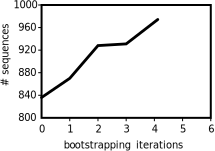
\includegraphics{Body/Images-chap2/growth.pdf}
        \caption[Graph of the progress of the bootstrapping method.]{
            A plot of the progress of the bootstrapping method.  The figure
            shows that our antimicrobial sequence database grew from 836 sequences
            to 931 sequences in 3 iterations.
        }
        \label{fig:bootProgress}
        \end{figure}

    \subsection{Annotator design and validation}
    Together, these $\sim$200K grammars describe the ``language'' of the
    AmP sequences.  In this linguistic metaphor, the peptide sequences are
    analogous to sentences and the individual amino acids are analogous to
    the words in a sentence.  Each grammar describes a common arrangement
    of amino acids, similar to popular phrases in English.

    Given an arbitrary sequence of amino acids, it is possible that
    some parts of the sequence are ``matched'' by one or more of the
    grammars in our database.  For example, the white mustard plant
    AmP Afp1 (Genbank accession no.\ P30231) contains the amino acid
    sequence fragment \texttt{CICYFPC}, which matches the grammar
    \texttt{CICY[FVK]PC} from our database.  (As discussed in Section~\vref{section:regex},
    the bracketed expression
    \texttt{[FVK]} indicates that, at the fifth position in the grammar,
    either phenylalanine, valine, or lysine is equally acceptable.)  Based on
    this match, we would say that the Afp1 fragment is ``grammatical.''


        Using the antimicrobial grammar database, we created an on--line tool
        for annotating antimicrobial peptides by determining the degree to which
        a query sequence is grammatical.  (This tool is
        available online at
        \url{http://cbcsrv.watson.ibm.com/Tspd.html}.)
        A user--supplied input sequence is annotated by generating grammar--based alignments
        of the input against sequences in our database of known antimicrobial
        sequences ($S$).  This alignment takes place
        in two distinct steps.  First, we search the input sequence for instances
        of grammars from the antimicrobial grammar database (the final $\phi'$).
        Second, for each contiguous stretch of shared grammars between the input
        sequence and a sequence from $S$, an alignment is produced.  Figure~\ref{fig:alignment}
        show a schematic of the alignment process.


        \begin{figure}[ptb]
        \centering
        \includegraphics{Body/Images-chap2/alignment.pdf}
        \caption[Schematic of the grammar--based alignment method]{
            A schematic of our grammar--based alignment method.  In the figure, a user--supplied
            input sequence is searched for instances of grammars ($p_A,p_B,p_C$\ldots) that occur
            in the set of known antimicrobial sequences ($S$).  Grammars that occur in both the
            input sequence and sequences in  $S$ are then used to create alignments.  As indicated in
            the figure, the input sequence shows homology to $s_1$ in two distinct regions, so
            both possible alignments are shown.  See
            Figure~\vref{fig:ampAlign} for an example of how these
            grammar--based alignments appear in practice.
        }
        \label{fig:alignment}
        \end{figure}

        \begin{sidewaysfigure}[ptb]
        \centering
        \includegraphics[width=\textheight]{Body/Images-chap2/amp-align.pdf}
        \caption[Example results of the grammar--based alignment method]{
            Example results of the grammar--based alignment method.
            The figure shows the annotation of a query sequence
            after it has been searched exhaustively for grammars in
            our database of $\sim$200K grammars describing the
            ``language'' of AmPs.  This alignment was generated
            using the methodology detailed in
            Figure~\vref{fig:alignment}.  Each of the sequences
            below the query is an AmP sequence from our database,
            $S$.  The sequences are aligned against the query
            because they share grammars in common at those
            particular loci.  However, different sequences may share
            very in degrees of conservation, even if they have the
            same grammar.  For example, see Figure~\vref{table:cons}.
        }
        \label{fig:ampAlign}
        \end{sidewaysfigure}

        \begin{sidewaystable}[ptbh]
    \caption[Motif conservation]{Motif conservation for the query shown in Figure and the motif \texttt{L[VQH][ALV][KLPQ][AS][EAF][APQS][ALRV]QA}.}
	\label{table:cons}
	\centering 
    \begin{tabular}{lllll} \hline\hline
QUERY		&	\texttt{LQAQAEPLQA}\\	\hline
P17534	&	\texttt{LVLLAFQVQA}	&	40.00\%	&	Cryptdin-related protein 4C-1	&	  Mus musculus (Mouse). \\
P19660	&	\texttt{LVLPSASAQA}	&	30.00\%	&	Bactenecin 5 precursor (BAC5)	&	  Bos taurus (Bovine). \\
P19661	&	\texttt{LVLPSASAQA}	&	30.00\%	&	Bactenecin 7 precursor (BAC7)	&	  Bos taurus (Bovine). \\
P28309	&	\texttt{LVLLSFQVQA}	&	30.00\%	&	Cryptdin-2 precursor	&	  Mus musculus (Mouse). \\
P28310	&	\texttt{LVLLAFQVQA}	&	40.00\%	&	Cryptdin-3 precursor	&	  Mus musculus (Mouse). \\
P28311	&	\texttt{LVLLAFQVQA}	&	40.00\%	&	Cryptdin-4 precursor	&	  Mus musculus (Mouse). \\
P28312	&	\texttt{LVLLAFQVQA}	&	40.00\%	&	Cryptdin-5 precursor	&	  Mus musculus (Mouse). \\
P32195	&	\texttt{LVVPSASAQA}	&	30.00\%	&	Protegrin 2 precursor (PG-2)	&	  Sus scrofa (Pig). \\
P33046	&	\texttt{LVVPSASAQA}	&	30.00\%	&	Indolicidin precursor	&	  Bos taurus (Bovine). \\
P49930	&	\texttt{LVVPSASAQA}	&	30.00\%	&	Antibacterial peptide PMAP-23	&	  Sus scrofa (Pig). \\
P49931	&	\texttt{LVVPSASAQA}	&	30.00\%	&	Antibacterial peptide PMAP-36	&	  Sus scrofa (Pig). \\
P49932	&	\texttt{LVVPSASAQA}	&	30.00\%	&	Antibacterial peptide PMAP-37	&	  Sus scrofa (Pig). \\
P50704	&	\texttt{LVLLAFQVQA}	&	40.00\%	&	Cryptdin-6/12 precursor	&	  Mus musculus (Mouse). \\
P50705	&	\texttt{LVLLAFQVQA}	&	40.00\%	&	Cryptdin-7 precursor	&	  Mus musculus (Mouse). \\
P50707	&	\texttt{LVLLAFQVQA}	&	40.00\%	&	Cryptdin-9 precursor	&	  Mus musculus (Mouse). \\
P50708	&	\texttt{LVLLAFQVQA}	&	40.00\%	&	Cryptdin-10 precursor (Fragmen	&	  Mus musculus (Mouse). \\
P50711	&	\texttt{LVLLAFQVQA}	&	40.00\%	&	Cryptdin-13 precursor	&	  Mus musculus (Mouse). \\
P50712	&	\texttt{LVLLAFQVQA}	&	40.00\%	&	Cryptdin-14 precursor (Fragmen	&	  Mus musculus (Mouse). \\
P50713	&	\texttt{LVLLAFQVQA}	&	40.00\%	&	Cryptdin-15 precursor	&	  Mus musculus (Mouse). \\
P50714	&	\texttt{LVLLAFQVQA}	&	40.00\%	&	Cryptdin-16 precursor	&	  Mus musculus (Mouse). \\
P51525	&	\texttt{LVVPSASAQA}	&	30.00\%	&	Prophenin-2 precursor (PF-2) (	&	  Sus scrofa (Pig). \\
P82270	&	\texttt{LHAQAEARQA}	&	70.00\%	&	Theta defensin-1, subunit A pr	&	  Macaca mulatta (Rhesus macaque). \\
P82271	&	\texttt{LHAQAEARQA}	&	70.00\%	&	Theta defensin-1, subunit B pr	&	  Macaca mulatta (Rhesus macaque). \\
P82318	&	\texttt{LQAQAEPLQA}	&	100.00\%	&	Neutrophil defensins 1, 3 and	&	  Macaca mulatta (Rhesus macaque). \\
Q01524	&	\texttt{LQAKAEPLQA}	&	90.00\%	&	Defensin 6 precursor (Defensin	&	  Homo sapiens (Human). 
	\\ \hline\hline
	\end{tabular}
	\end{sidewaystable}


    Since it is possible that, for an arbitrary sequence, only a portion
    of the sequence is matched by one of our grammars, we developed a
    heuristic metric $Z$, which is the degree to which a query sequence
    is grammatical.  To calculate $Z$, we assign a local score along the
    backbone of a query sequence that is equal to the number of grammars,
    or fractions of grammars with at least 10 amino acids, that have
    matches over the length of the query sequence.  The total score for
    the sequence, $Z$, is the fraction of the sequence's length that
    is covered by at least one grammar (see Figure~1\ref{fig:space}).
    For example, a hypothetical sequence \texttt{LFLTAIDRYIAAA} ---
    which is matched by \texttt{LFLTAI[ID][TR][VY]I}, but no other
    grammars in our database --- would get a score of 10/13 since the
    first 10 positions in the sequence are covered by the match.

    In order to annotate and design synthetic AmPs, we created a software tool to
    calculate the score $Z$ for a query sequence and to classify the
    sequence as either likely to have antimicrobial activity --- if its
    $Z$--score is above a certain threshold --- or not.  To determine
    this threshold, we trained the tool on a subset of sequences from our
    AmP database as follows.  We randomly selected $90\%$ of the natural
    AmP sequences and generated a Teiresias grammar set, using the same
    Teiresias parameters that were used to generate our $\sim$200K grammar
    set.  This smaller grammar set was used by our software to classify
    the remaining $10\%$ of our AmP database, which was hidden among
    $10\%$ of the non--AmP sequences from Swiss--Prot/TrEMBL ($\sim$78K
    sequences).  This experiment was repeated 300 times, with different
    random sets, to determine the best $Z$--score.  We found that, at
    an $Z$--score threshold of 0.73, the software tool will correctly
    classify both the AmP and non--AmP sequences with $99.95$\% accuracy.


\section{Preliminary strategy for the design of novel
AmPs}\label{section:preliminary}

    \subsection{Sequence design}
    As I showed in the previous section, the $Z$--score annotation
    metric is both sensitive and selective for existing AmPs.
    We hypothesized that this metric could be used equally well to
    design unnatural sequences that would have antimicrobial
    activity.  In this section, I describe our preliminary strategy
    for designing these novel, unnatural sequences.
    \textit{Notably, the experimental data presented
    in this section were later discovered to not be
    reproducible due to experimental complications. See
    Section~\vref{section:fake}.  The data are presented
    here for the insight they lend to our more focused,
    and successful, strategy for designing AmPs, which is
    described in Section~\vref{section:focused}.}

    Based on the annotation results described in the previous
    section,
    we ran a computer simulation to create novel amino acid sequences
    with high $Z$--scores, but with minimal homology to natural AmPs.
    This simulation, shown schematically in Figure~\vref{fig:evolution},
    used the $Z$--score as a fitness function for the \emph{in
    silico} directed evolution of these novel sequences.  To begin,
    we created a randomized database of 100K progenitor sequences
    of uniform length with the same amino acid composition (i.e.,
    the same percentage of each amino acid type) as our AmP database.
    Each of these sequences was allowed to have 4 mutated ``children,''
    which were each 100 PAM (point accepted mutations) evolutionary
    units away from the parent.  (The implied rates of mutation from
    the Blosum--50 matrix were used to make the mutations at the amino
    acid level~\cite{henikoff1992aminoacid}.)  These children, each
    of which differed from their parent sequence by at least one amino
    acid, were added to the total population of sequences.  In order to
    avoid generating sequences that were similar to natural AmPs, the
    population was purged of any sequences that had 6 or more consecutive
    amino acids in common with any natural AmP sequence.  Finally,
    the remaining sequences were scored using our annotation software.
    From the population, the sequences with the top 100 $Z$--scores
    were propagated to the following round, and the entire process was
    repeated.


        \begin{figure}
        \centering
        \includegraphics[width=\textwidth]{Body/Images-chap2/evolution.pdf}
        \caption[Directed evolution]{ A schematic of the \emph{in
        silico} directed evolution strategy.  Position (1)
        shows the starting point: the database of 100K parental
        sequences.  Each of these sequences has 4 mutated
        children (2) and the entire population is scored using the
        $Z$--score and our database of grammars from natural AmPs.
        From the scored population (3), the top 100 sequences
        are chosen and become the parental sequences for the
        next iteration.  In addition to the directed evolution
        simulation, we considered other methods for generating
        sequences with high $Z$--scores.  However, we chose this
        approach because it naturally allows for sequences of
        arbitrary length and the possibility that grammars may
        overlap in the designed amino acid sequences.}%
        \label{fig:evolution}
        \end{figure}

    Using the strategy described above, we allowed many populations
    of sequences to evolve, each with a different sequence length,
    which remained constant during the simulation.  We stopped each
    simulation after $3,000$ rounds of mutation and selection, by which
    point we found that populations of small sequence length would have
    converged to $S=1$.  For longer length populations, all the sequences
    typically reached at least $S=0.73$ and all tended to be closely
    related to each other.  We chose three sequences of lengths 20, 31,
    and 63 amino acids to test experimentally for antimicrobial activity:
    sequences synth--1, 2, and 3 in Table~\vref{table:peptides}.



\begin{sidewaystable}[ptbh]
    \caption[The preliminary design synthetic antimicrobial peptides used in this study]{The preliminary design synthetic antimicrobial peptides used in this study
	For each synthetic AmP we also designed two sequences
	(``negative'' a and b), which have the same amino acid
	composition as the synthetic peptide but have an $S$--score
	of zero.  The table also shows statistics relavant to
	AmPs, which were calculated using the EMBOSS software
	package\cite{rice2000emboss}.  Note that synth--3 has only
	one negative version.  Also, the peptides synth--1, 2, and 3
	were the \emph{only} peptides designed using our grammatical
	approach that were synthesized and tested experimentally.
        }\label{table:peptides} \begin{center} 
    \begin{tabular}{lccccl} \hline \hline
	Peptide &  S & Size & Charge & pI & Sequence\\ \hline
	\textbf{synth--1:} &  & 20 & 4.5 & 11.92\\
	~~~synth--1 & 1 &  &  &  & {\footnotesize \ttfamily NKVKKPLTGAHRLLFTFLFV} \\
	~~~negative--1a & 0 &  &  &  & {\footnotesize \ttfamily VVLKLLFFKFNLPHKTRTAG} \\
	~~~negative--1b & 0 &  &  &  & {\footnotesize \ttfamily LVLTFLFATPKLNGRVKKFH} \\
	\textbf{synth--2:} &  & 31 & 10.0 & 11.28 \\
	~~~synth--2  & 1 &  &  &   & {\footnotesize \ttfamily MKKIKKEAGKNILKLAPKEVAAKKSKKSPTK} \\
	~~~negative--2a  & 0 &  &  &   & {\footnotesize \ttfamily PAAGESKVKANKKKAKILPTMKLKKEIKKKS} \\
	~~~negative--2b  & 0 &  &  & 	& {\footnotesize \ttfamily SEASLKAKIKKIAMKKVTKGKAKNKPKLPEK} \\
	\textbf{synth--3:}&  & 63 & 3.0 & 10.41\\
	~~~synth--3 & 0.92 &  &  &   & {\footnotesize \ttfamily MKDKNSTGPLLSALLLAVTAGGSPVAAAPWNPFAAILKAALQIAGAAEPKEVTAKKGPTKADA}\\
	~~~negative--3a & 0 &  &  &  & {\footnotesize \ttfamily GWAGLVAETAIADKMSLKAAGEPPNQNDGAVLKTPPKAAASAKPLGAAKTLAFISPVTLALAK}\\
	%~~~negative--3b & 0 & 63 & 3.0 & 10.41  & {\footnotesize \ttfamily AAKGVAAAPEANALSAWTTPMGLGGSIGFDKPPKKALKNKLTPAAVKSVLLPALATIAQEDAA}
	\\ \hline\hline
    \end{tabular} \end{center}

 \end{sidewaystable}




    Using NCBI Blast~\cite{altschul1997gapped} (blastp) with the default
    parameters, we compared these sequences to the entire NCBI NR
    sequence database.  The Blast results showed that none of the three
    sequences has significant homology to \emph{any} known protein
    (E--value $\leq$10), including the naturally--occurring AmPs.
    (More extensive similarity searching using PSI--Blast and E--value
    thresholds up to $\leq$50 also failed to detect similarity to any
    natural AmPs.)  This is possible because each grammar can be written
    in a large number of ways.  For example, the 10--residue grammar
    \texttt{[LV][GA]K[TN][FL]AGHML} occurs in 3 natural AmPs, but there
    are 16 possible 10--residue sequences that match this grammar.
    Since our sequences are built from tiled grammars, the synthetic
    sequences can quickly deviate from the naturally populated sequence
    space such that it is impossible to detect similarity using sequence
    alignment tools (see Figure~\vref{fig:space}).



        \begin{figure}
        \centering
        \includegraphics[width=0.75\textwidth]{Body/Images-chap2/space.pdf}
        \caption[Design space]{ The AmP design space.
        Part A shows the sequence space surrounding the set of
        natural AmPs.  The ``sequence space'' is the combinatorially
        large set of all possible sequences.  Even for a 20--residue
        peptide like synth--1 (see Table~\ref{table:peptides})
        this space is huge: $20^{20}\approx 10^{26}$ sequences.
        (For comparison, there are about $10^{22}$ stars in the known
        universe.)  Our linguistic model focuses the search space to
        the ``grammar space,'' but allows a deviation from natural
        AmP sequences.  This allows us to design peptides that show
        no significant homology to any naturally occurring sequences,
        but have the desired function.  Part B shows a subsequence
        of the synth--2 peptide.  Above and below the subsequence
        are grammars that match the sequence in a tiled arrangement.
        For each bracketed expression, any of the amino acids listed
        in the bracket will suffice.}
        \label{fig:space}
    \end{figure}


    For each of the three synthetic peptides, we also designed a
    set of shuffled sequences, which we hypothesized would have no
    antimicrobial activity.  These ``negative'' peptides are shown along
    with the three synthetic peptides in Table~\ref{table:peptides}.
    The negative peptides have the same amino acids as the synthetic
    sequences (and thus, the same molecular weight, charge, and pI);
    however, the order of the amino acids was shuffled so that the
    negative sequences each have an $Z$--score of zero.



\subsection{Peptide synthesis and validation}
    Using an approach described elsewhere~\cite{martemyanov2001cell}, we
    synthesized all 8 of the peptides shown in Table~\ref{table:peptides}.
    For each peptide we created a translation template
    consisting of three parts: green fluorescent protein (GFP) with a
    T7 promoter, an enterokinase recognition site (ERS), and the AmP to
    be tested.  We synthesized the protein--product of each template in
    an \emph{E. coli}--derived \emph{in vitro} translation system
    with continuous exchange~\cite{kim1996semicontinuous}.  The resulting
    peptides were proteolytically cleaved with enterokinase and the yield
    of AmP in the translation mixture was measured via GFP fluorescence
    using a 1:1 molar equivalence between the AmP and GFP concentrations.

    We characterized the antimicrobial activity of each
    synthetic AmP using a broth microdilution assay described
    previously~\cite{amsterdam1996susceptibility}.  The top
    section of Table~\ref{table:results} shows the activities of the
    synthetic peptides against four bacterial species: \emph{Bacillus
    cereus}, \emph{Corynebacterium glutamicum}, \emph{E. coli}, and
    \emph{Citrobacter rodentium}.  (See also Figure~\vref{fig:graph2}.)
    These data suggested that all three synthetic peptides
    had antimicrobial activity.  Furthermore, none of the negative,
    ``un--grammatical'' sequences had any activity.  Thus, it appeared that the activity
    of the designed peptides was not an artifact of molecular weight,
    charge, or pI\@.  Instead, the activity appeared correlated to the $Z$--score,
    suggesting that higher order sequence features are responsible for
    antimicrobial activity.  (\emph{These data were later shown to be
    not reproducible.  Later experiments showed that the
    sequences in Table~\ref{table:results} did not have
    detectable levels of antimicrobial
    activity under a more stringent assay. See Section~\vref{section:fake}.})

    The bottom of Table~\ref{table:results} shows the measured activities of
    synth--1 variants that were synthesized chemically --- the peptides
    were purchased in 70\% minimum purity from Invitrogen (Carlsbad, CA)
    --- instead of by our \emph{in vitro} method.  As shown, the activity
    profiles for these peptides appeared to match their \emph{in vitro}--synthesized
    counterparts, suggesting that the antimicrobial activity was not
    a relic of the translation mixture.  (We also used the chemically
    synthesized copy of synth--1 to validate the size of our \emph{in
    vitro} synthesized copy; see Figure~3\ref{fig:gel}.)  Furthermore,
    we found that luciferase (a luminescent protein with no antimicrobial
    characteristics), when synthesized via our \emph{in vitro} method,
    had no activity.  Thus, we were confident that the translation mixture
    had no innate antimicrobial activity that may have produced spurious
    results.

        \begin{figure}
        \centering
        \includegraphics[width=0.95\textwidth]{Body/Images-chap2/detailed-graph.pdf}
        \caption[Antimicrobial peptide action]{Bacteriostatic activity
        of the three synthetic AmPs against \emph{B. cereus}.
        The breakouts show photographs of the colonies, which
        decreased
        in number with increasing peptide concentration.  The inlaid
        schematic shows the generally accepted mechanism of AmP
        action: the electrostatic affinity for the outer--leaflet
        of the bacterial membrane leads to binding and rupture of
        the cell~\cite{shai2002mode}.
        (\emph{These data were later shown to be
    not reproducible.  Later experiments showed that 
    these
    peptides had undetectable levels of antimicrobial
    activity under a more reliable antimicrobial assay. See Section~\vref{section:fake}.})}
        \label{fig:graph2}
    \end{figure}


        \begin{figure}
        \centering
        \includegraphics{Body/Images-chap2/control-gel.pdf}
        \caption[Gel picture]{SDS--PAGE gel showing the synth--1
        \emph{in vitro} translation product (lane B).  Lane
        A shows the translation mixture with no peptide and
        lane C shows the *synth--1 peptide, which was produced
        via solid phase synthesis and validated by mass
        spectroscopy.}
        \label{fig:gel}
    \end{figure}



\begin{sidewaystable}[ptbh]
    \caption[Antimicrobial activity of the synthetic peptides against a variety of bacteria]{Antimicrobial activity of the synthetic peptides against a variety of bacteria.
	Each entry in the table shows the relative viability of
	the bacteria: the ratio of the cell count at a particular
	concentration of AmP to the cell count at 0 $\mu$g/mL.  The entries
	in dark gray show high viability (low antimicrobial action) and the
	white entries show low viability (high antimicrobial action).
	The names prepended with a ``*'' are peptides that were chemically
	synthesized rather than produced via \emph{in vitro} translation.
	    }\label{table:results} \begin{center} %\scriptsize
    %\begin{tabular}{lcccc|cccc|cccc|cccc} \hline \hline
    \begin{tabular}{lc@{\extracolsep{0.0mm}}c@{\extracolsep{0.0mm}}c@{\extracolsep{0.0mm}}c@{\extracolsep{2mm}} c@{\extracolsep{0.0mm}}c@{\extracolsep{0.0mm}}c@{\extracolsep{0.0mm}}c@{\extracolsep{2mm}} c@{\extracolsep{0.0mm}}c@{\extracolsep{0.0mm}}c@{\extracolsep{0.0mm}}c@{\extracolsep{2mm}}c@{\extracolsep{0.0mm}}c@{\extracolsep{0.0mm}}c@{\extracolsep{0.0mm}}c@{\extracolsep{0.0mm}}}% \hline \hline
	species $\rightarrow$	
	& \multicolumn{4}{c}{ \underline { \emph{B. subtilis} }}
	& \multicolumn{4}{c}{ \underline {\emph{C. glutamicum} }}
	& \multicolumn{4}{c}{ \underline {\emph{E. coli} }}
	& \multicolumn{4}{c}{ \underline {\emph{C. rodentium} }}\\
	peptide conc. ($\mu$g/mL) $\rightarrow$ & 0 & 5 & 10 & 15
	& 0 & 5 & 10 & 15
	& 0 & 5 & 10 & 15
	& 0 & 5 & 10 & 15\\ %\hline
	\textbf{synth--1:}\\
	%~~synth--1 & 1.00 &  0.80 & 0.08 & 0.03 & 1.00 & 0.73 & 0.21 & 0.15 &  1.00 & 1.02 & 1.00 &   0.93 & 1.00 &  0.99  &  0.97  &  0.98 \\
	%~~negative--1a & 1.00 & 0.96 & 1.01 & 1.00 & 1.00 & 1.00 & 0.93 & 1.01 & 1.00 & 1.00 & 0.99 & 1.02 & 1.00 & 0.99 & 1.01 & 0.98 \\
	%~~negative--1b & 1.00 & 0.98 & 1.03 & 1.02 & 1.00 & 1.01 & 0.96 & 0.99 & 1.00 & 1.01 & 0.98 & 0.99 & 1.00 & 1.01 & 1.02 & 1.01 \\
	~~synth--1 & \colorbox[gray]{0.500}{1.00}  & \colorbox[gray]{0.600}{0.80}  & \colorbox[gray]{0.960}{0.08}  & \colorbox[gray]{0.985}{0.03}  & \colorbox[gray]{0.500}{1.00}  & \colorbox[gray]{0.635}{0.73}  & \colorbox[gray]{0.895}{0.21}  & \colorbox[gray]{0.925}{0.15}  & \colorbox[gray]{0.500}{1.00}  & \colorbox[gray]{0.500}{1.00}  & \colorbox[gray]{0.500}{1.00}  & \colorbox[gray]{0.535}{0.93}  & \colorbox[gray]{0.500}{1.00}  & \colorbox[gray]{0.505}{0.99}   & \colorbox[gray]{0.515}{0.97}   & \colorbox[gray]{0.510}{0.98}  \\

	~~negative--1a & \colorbox[gray]{0.500}{1.00}  & \colorbox[gray]{0.520}{0.96}  & \colorbox[gray]{0.500}{1.00}  & \colorbox[gray]{0.500}{1.00}  & \colorbox[gray]{0.500}{1.00}  & \colorbox[gray]{0.500}{1.00}  & \colorbox[gray]{0.535}{0.93}  & \colorbox[gray]{0.500}{1.00}  & \colorbox[gray]{0.500}{1.00}  & \colorbox[gray]{0.500}{1.00}  & \colorbox[gray]{0.505}{0.99}  & \colorbox[gray]{0.500}{1.00}  & \colorbox[gray]{0.500}{1.00}  & \colorbox[gray]{0.505}{0.99}  & \colorbox[gray]{0.500}{1.00}  & \colorbox[gray]{0.510}{0.98}  \\

	~~negative--1b & \colorbox[gray]{0.500}{1.00}  & \colorbox[gray]{0.510}{0.98}  & \colorbox[gray]{0.500}{1.00}  & \colorbox[gray]{0.500}{1.00}  & \colorbox[gray]{0.500}{1.00}  & \colorbox[gray]{0.500}{1.00}  & \colorbox[gray]{0.520}{0.96}  & \colorbox[gray]{0.505}{0.99}  & \colorbox[gray]{0.500}{1.00}  & \colorbox[gray]{0.500}{1.00}  & \colorbox[gray]{0.510}{0.98}  & \colorbox[gray]{0.505}{0.99}  & \colorbox[gray]{0.500}{1.00}  & \colorbox[gray]{0.500}{1.00}  & \colorbox[gray]{0.500}{1.00}  & \colorbox[gray]{0.500}{1.00}  \\




	\textbf{synth--2:}\\
	%~~synth--2 & 1.00 & 0.27 & 0.03  & 0.02 & 1.00 & 0.28 & 0.21 &  0.12 & 1.00 & 1.01 &  1.01 & 0.99 & 1.00 & 0.99 & 0.99 & 0.97 \\
	%~~negative--2a  & 1.00 & 1.02 & 1.00 & 1.02 & 1.00 & 1.01 & 0.96 & 0.91 & 1.00 & 0.98 & 0.99 & 1.01 & 1.00 & 0.95 & 0.99 & 0.95 \\
	%~~negative--2b  & 1.00 & 1.01 & 1.02 & 1.01 & 1.00 & 0.92 & 0.95 & 0.98 & 1.00 & 0.98 & 0.97 & 0.97 & 1.00 & 0.98 & 0.94 & 0.99 \\
	~~synth--2 & \colorbox[gray]{0.500}{1.00}  & \colorbox[gray]{0.865}{0.27}  & \colorbox[gray]{0.985}{0.03}   & \colorbox[gray]{0.990}{0.02}  & \colorbox[gray]{0.500}{1.00}  & \colorbox[gray]{0.860}{0.28}  & \colorbox[gray]{0.895}{0.21}  & \colorbox[gray]{0.940}{0.12}  & \colorbox[gray]{0.500}{1.00}  & \colorbox[gray]{0.500}{1.00}  & \colorbox[gray]{0.500}{1.00}  & \colorbox[gray]{0.505}{0.99}  & \colorbox[gray]{0.500}{1.00}  & \colorbox[gray]{0.505}{0.99}  & \colorbox[gray]{0.505}{0.99}  & \colorbox[gray]{0.515}{0.97}  \\

	~~negative--2a  & \colorbox[gray]{0.500}{1.00}  & \colorbox[gray]{0.500}{1.00}  & \colorbox[gray]{0.500}{1.00}  & \colorbox[gray]{0.500}{1.00}  & \colorbox[gray]{0.500}{1.00}  & \colorbox[gray]{0.500}{1.00}  & \colorbox[gray]{0.520}{0.96}  & \colorbox[gray]{0.545}{0.91}  & \colorbox[gray]{0.500}{1.00}  & \colorbox[gray]{0.510}{0.98}  & \colorbox[gray]{0.505}{0.99}  & \colorbox[gray]{0.500}{1.00}  & \colorbox[gray]{0.500}{1.00}  & \colorbox[gray]{0.525}{0.95}  & \colorbox[gray]{0.505}{0.99}  & \colorbox[gray]{0.525}{0.95}  \\

	~~negative--2b  & \colorbox[gray]{0.500}{1.00}  & \colorbox[gray]{0.500}{1.00}  & \colorbox[gray]{0.500}{1.00}  & \colorbox[gray]{0.500}{1.00}  & \colorbox[gray]{0.500}{1.00}  & \colorbox[gray]{0.540}{0.92}  & \colorbox[gray]{0.525}{0.95}  & \colorbox[gray]{0.510}{0.98}  & \colorbox[gray]{0.500}{1.00}  & \colorbox[gray]{0.510}{0.98}  & \colorbox[gray]{0.515}{0.97}  & \colorbox[gray]{0.515}{0.97}  & \colorbox[gray]{0.500}{1.00}  & \colorbox[gray]{0.510}{0.98}  & \colorbox[gray]{0.530}{0.94}  & \colorbox[gray]{0.505}{0.99}  \\



	\textbf{synth--3:}\\
	%~~synth--3 & 1.00 & 0.39 & 0.11 & 0.07 & 1.00 & 0.40 & 0.26 & 0.18 & 1.00 & 1.05 & 1.02 & 0.99 & 1.00 & 1.00 & 0.98 & 0.10 \\
	%~~negative--3a & 1.00 & 0.96 & 0.98 & 0.98 & 1.00 & 1.01 & 0.96 & 0.96 & 1.00 & 1.00 & 1.00 & 0.99 & 1.00 & 1.01 & 0.96 & 0.96 \\
	~~synth--3 & \colorbox[gray]{0.500}{1.00}  & \colorbox[gray]{0.805}{0.39}  & \colorbox[gray]{0.945}{0.11}  & \colorbox[gray]{0.965}{0.07}  & \colorbox[gray]{0.500}{1.00}  & \colorbox[gray]{0.800}{0.40}  & \colorbox[gray]{0.870}{0.26}  & \colorbox[gray]{0.910}{0.18}  & \colorbox[gray]{0.500}{1.00}  & \colorbox[gray]{0.500}{1.00}  & \colorbox[gray]{0.500}{1.00}  & \colorbox[gray]{0.505}{0.99}  & \colorbox[gray]{0.500}{1.00}  & \colorbox[gray]{0.500}{1.00}  & \colorbox[gray]{0.510}{0.98}  & \colorbox[gray]{0.950}{0.10}  \\

	~~negative--3a & \colorbox[gray]{0.500}{1.00}  & \colorbox[gray]{0.520}{0.96}  & \colorbox[gray]{0.510}{0.98}  & \colorbox[gray]{0.510}{0.98}  & \colorbox[gray]{0.500}{1.00}  & \colorbox[gray]{0.500}{1.00}  & \colorbox[gray]{0.520}{0.96}  & \colorbox[gray]{0.520}{0.96}  & \colorbox[gray]{0.500}{1.00}  & \colorbox[gray]{0.500}{1.00}  & \colorbox[gray]{0.500}{1.00}  & \colorbox[gray]{0.505}{0.99}  & \colorbox[gray]{0.500}{1.00}  & \colorbox[gray]{0.500}{1.00}  & \colorbox[gray]{0.520}{0.96}  & \colorbox[gray]{0.520}{0.96}  \\



	\\
	\textbf{Chemically synthesized:}\\
	%~~*synth--1 & 1.00 & 0.72 & 0.14 & 0.14 & 1.00 & 0.56 & 0.16 & 0.11 & 1.00 & 0.89 & 0.92 & 0.86 & 1.00 & 0.90 & 0.90 & 0.90 \\
	%~~*negative--1a & 1.00 & 1.04 & 0.84 & 0.87 & 1.00 & 1.01 & 1.04 & 1.10 & 1.00 & 0.92 & 0.90 & 0.94 & 1.00 & 1.03 & 0.98 & 1.01 \\
	%~~*negative--1b & 1.00 & 0.92 & 0.98 & 0.96 & 1.00 & 1.00 & 0.96 & 1.02 & 1.00 & 1.00 & 1.01 & 0.97 & 1.00 & 1.02 & 1.02 & 1.02 \\
	~~*synth--1 & \colorbox[gray]{0.500}{1.00}  & \colorbox[gray]{0.640}{0.72}  & \colorbox[gray]{0.930}{0.14}  & \colorbox[gray]{0.930}{0.14}  & \colorbox[gray]{0.500}{1.00}  & \colorbox[gray]{0.720}{0.56}  & \colorbox[gray]{0.920}{0.16}  & \colorbox[gray]{0.945}{0.11}  & \colorbox[gray]{0.500}{1.00}  & \colorbox[gray]{0.555}{0.89}  & \colorbox[gray]{0.540}{0.92}  & \colorbox[gray]{0.570}{0.86}  & \colorbox[gray]{0.500}{1.00}  & \colorbox[gray]{0.550}{0.90}  & \colorbox[gray]{0.550}{0.90}  & \colorbox[gray]{0.550}{0.90}  \\

	~~*negative--1a & \colorbox[gray]{0.500}{1.00}  & \colorbox[gray]{0.500}{1.00}  & \colorbox[gray]{0.580}{0.84}  & \colorbox[gray]{0.565}{0.87}  & \colorbox[gray]{0.500}{1.00}  & \colorbox[gray]{0.500}{1.00}  & \colorbox[gray]{0.500}{1.00}  & \colorbox[gray]{0.500}{1.00}  & \colorbox[gray]{0.500}{1.00}  & \colorbox[gray]{0.540}{0.92}  & \colorbox[gray]{0.550}{0.90}  & \colorbox[gray]{0.530}{0.94}  & \colorbox[gray]{0.500}{1.00}  & \colorbox[gray]{0.500}{1.00}  & \colorbox[gray]{0.510}{0.98}  & \colorbox[gray]{0.500}{1.00}  \\

	~~*negative--1b & \colorbox[gray]{0.500}{1.00}  & \colorbox[gray]{0.540}{0.92}  & \colorbox[gray]{0.510}{0.98}  & \colorbox[gray]{0.520}{0.96}  & \colorbox[gray]{0.500}{1.00}  & \colorbox[gray]{0.500}{1.00}  & \colorbox[gray]{0.520}{0.96}  & \colorbox[gray]{0.500}{1.00}  & \colorbox[gray]{0.500}{1.00}  & \colorbox[gray]{0.500}{1.00}  & \colorbox[gray]{0.500}{1.00}  & \colorbox[gray]{0.515}{0.97}  & \colorbox[gray]{0.500}{1.00}  & \colorbox[gray]{0.500}{1.00}  & \colorbox[gray]{0.500}{1.00}  & \colorbox[gray]{0.500}{1.00}  \\




     \\ %\hline\hline
    \end{tabular} \end{center} 

	\end{sidewaystable}









    For each peptide/organism combination, we measured a minimum
    inhibitory concentration (MIC) at which 80\% of colony growth
    was inhibited (see Table~\ref{table:mic}).
    Many of the peptides appeared to exhibit strong bacteriostatic activity
    (MIC$_{80}\leq8$ $\mu$g/mL).  For example, all of the peptides
    seemed highly active against \emph{B. cereus}.  However, with
    the exception of synth--3, all of the AmPs appeared specific to
    gram--positive bacteria.  Such specificity is a common characteristic
    of natural AmPs.  For example, the insect cecropins are usually
    specific to gram--positive bacteria~\cite{shai2002mode}; whereas,
    the honey bee AmP apidaecin is active only against gram negative
    bacteria~\cite{casteels1994apidaecin}.  In general, the underlying
    reasons for the variations in the susceptibilities of different
    bacterial species is unknown~\cite{zasloff2002antimicrobial}.


\begin{table}[ptbh]
    \caption[Minimum inhibitory concentration of the preliminary design synthetic AmPs against a variety of bacteria]{Minimum inhibitory concentration of the preliminary design synthetic AmPs against a variety of bacteria.
	In the table MIC$_{50}$ is the concentration of peptide, in
	$\mu$g/mL, required to inhibit 50\% of the bacterial growth.
	A ``-'' indicates that the MIC is greater than 15 $\mu$g/mL.
	   }\label{table:mic}
    \begin{center}
    \footnotesize

    \begin{tabular}{lcccccc}% \hline \hline
	% first row
	& \multicolumn{2}{c}{ \underline{synth--1} }	
	& \multicolumn{2}{c}{ \underline{synth--2} }	
	& \multicolumn{2}{c}{ \underline{synth--3} }	\\
	% second row
	& \scriptsize MIC$_{50}$ & \scriptsize MIC$_{80}$
	& \scriptsize MIC$_{50}$ & \scriptsize MIC$_{80}$
	& \scriptsize MIC$_{50}$ & \scriptsize MIC$_{80}$ \\ %\hline
	% 
	\multicolumn{2}{l}{\bfseries Gram--positive:}\\
	% third row
	\emph{~~B. subtilis}
	& 7.5
	& 10
	& 3.5
	& 6
	& 4.5
	& 8.5\\
	% forth row
	\emph{~~C. glutamicum}
	& 4
	& 13.5
	& 3.5
	& 11
	& 4
	& 10\\ 
	% 
	\multicolumn{2}{l}{\bfseries Gram--negative:}\\
	% 
	\emph{~~E. coli}
	& -
	& -
	& -
	& -
	& -
	& -\\ 
	% 
	\emph{~~C. rodentium}
	& -
	& -
	& -
	& -
	& 12
	& 15\\ 
	%\hline\hline
    \end{tabular}
    \end{center}

\end{table}


    We selected the synth--1 family of peptides (*synth--1, *negative--1a,
    and *negative--1b in Table~\ref{table:peptides}) to characterize
    more thoroughly.  These peptides were tested at concentrations up to
    50 $\mu$g/mL (a typical MIC for moderately active naturally--occurring
    AmPs) against the gram--negative bacteria.  These additional experiments
    suggested that that *synth--1 was
    active against \emph{C.\ rodentium} at 50 $\mu$g/mL, preventing 99\%
    of the bacterial growth with an MIC$_{80}$ of roughly 40 $\mu$g/mL.
    However, *synth--1 was not active against \emph{E.\ coli} at this
    concentration.  As expected, the *negative--1a and *negative--1b
    peptides did not have any activity against either \emph{C.\ rodentium}
    or \emph{E.\ coli} at 50 $\mu$g/mL.

    In addition, we tested the synth--1 family of peptides for
    cooperativity with the polymyxin B nonapeptide, which is known
    to permeabilize the outer membrane of gram--negative bacteria.
    We found that the nonapeptide did not sensitize \emph{C.\ rodentium}
    or \emph{E.\ coli} to *synth--1, *negative--1a, or *negative--1b,
    suggesting that the outer membrane may not be the limiting factor
    in the activity of synth--1 against gram--negative bacteria.

    Finally, we measured the activity of the synth--1 family of peptides
    against human erythrocytes (see Figure~\vref{fig:hemolysis}).  Our results show that
    *negative--1a was moderately hemolytic and suggest an HM$_{50}$
    of approximately 60 $\mu g/mL$.  *Synth--1 and *negative--1b were
    less active against erythrocytes, with HM$_{50}$ concentrations
    (by extrapolation) of roughly 260 and 290 $\mu g/mL$, respectively.




        \begin{figure}
        \centering
        \includegraphics[width=0.95\textwidth]{Body/Images-chap2/hemolysis.pdf}
        \caption[Antimicrobial peptide hemolysis]{Activity
        of the synth--1 family of peptides against human
        erythrocytes determined using a procedure described
        elsewhere~\cite{liu2001denovo}.  The ordinate shows the
        degree of hemolysis relative to 50 $\mu$g/mL of melittin,
        which causes complete hemolysis.} \label{fig:hemolysis}
    \end{figure}





\subsection{Later experimentation}\label{section:fake}


    As mentioned briefly in the preceding sections, the experimental
    data suggesting that synth--1 had to antimicrobial activity,
    were later shown not to be reproducible.  Specifically, the
    *synth--1 peptide was shown to have no antimicrobial activity up
    to 50 $\mu g/mL$.  These experiments implied that the data for
    all of the synthetically generated peptides discussed in the
    previous section were suspect, with the exception of the data on
    the hemolytic potential of the peptides.  Based on these new
    findings, we revisited the AmP design problem and developed a
    more focused approach on the assumption that the original
    evolutionary methodology would not succeed.  In particular, the
    lack of activity by the *synth--1 peptide indicated that perhaps
    the $Z$--score was an inadequate metric for designing AmPs,
    despite its power for annotation.


\section{Focused design of AmPs}\label{section:focused}

\subsection{Derivation of highly conserved AmP grammars}

    In the previous section, I described a strategy for designing
    novel AmPs that have a strong emphasis on sensitivity.  That is,
    much effort was expended collecting a database of AmP sequences
    that was exhaustive so that the set of grammars derived from
    that database would be exhaustive as well
    (see Section~\vref{section:annotation}).  The
    annotation experiments suggest that this strategy is sensitive
    for discovering novel AmPs; however, the lack
    antimicrobial activity by *synth--1 suggests that perhaps this
    approach (and the metric $Z$) is not selective.  This lack of selectivity may be
    rooted in the exhaustive database of AmP sequences, which
    contains many sequences spanning a wide range of
    activities.  That is, there are some AmP sequences in the
    database that have very low activity and some with very high
    activity.  In addition, many of the sequences in this database
    are in precursor form.  For the sequences, the precursor
    undergoes a series of post translational modifications before
    yielding a mature, active antimicrobial peptide.  The regions of
    the proteins that are cleaved off, or otherwise not responsible
    for the antimicrobial activity of the peptide are essentially
    ``noise'' in the derived set of $\sim$200K grammars derived in
    the previous section.

    In order to focus instead on specificity, not sensitivity \emph{per se}, we
    decided to use a database of well--characterized eukaryotic AmP
    sequences from the Antimicrobial Peptide Database
    (APD)~\cite{wang2004apd}.  The APD is unique in that it is the
    only database of antimicrobial peptides that restricts the
    sequences it catalogs to only those for which there is a large
    body of experimental data confirming the activity of each AmP.
    Furthermore, the AmPs listed in the APD are mature in the sense
    that they are not precursor proteins.  Therefore, we know with
    high confidence that each sequence in the APD  has
    antimicrobial activity and that we are unlikely to be training
    on sequences that are not responsible in some part for this activity.

    As in Section~\vref{section:preliminary},
    we used the Teiresias pattern
    discovery tool to derive regular grammars that occur commonly
    in the set of 526 well--characterized eukaryotic AmP
    sequences from the APD\@.
    Using these APD sequences, we ran the Teiresias pattern discovery
    tool with the following settings: L = 6, W =
    6, and K = 2 (a detailed description of the
    Teiresias input parameters and associated tools
    is available in Section~\vref{section:teiresias}). The resulting grammar
    set was masked from the input sequences and the
    process was repeated using L = 7, W = 15, K = 5
    with the following amino acid equivalency groups
    \texttt{[[AG], [DE], [FYW], [KR], [ILMV], [QN], [ST]]}.
    The equivalency groups mean that Teiresias will consider any two
    characters in the same group to be exactly equivalent.  Thus, in
    the groups above alanine is treated exactly as glycine.  In
    effect, using equivalency groups allows us to find motifs that
    are more weakly conserved, but that have similar chemistries.
    (As I will show in Chapter~\vref{chapter:gemoda}, Teiresias
    is unable to use a more fine--grained metric for the similarity
    between two amino acids.  That is, Teiresias can only use
    equivalency groups to say ``equivalent'' or ``not equivalent''
    but it cannot use metrics such as ``alanine is five arbitrary
    units in a way from glycine, which is 10 arbitrary units away
    from leucine.)

As I discussed in Section~\vref{section:teiresias}, Teiresias
outputs its grammars in regular expression format, using wildcards.
To make the grammars more selective, we de--referenced each wildcard
in the grammars to a bracketed expression, using the same procedure
described in Section~\vref{section:annotation}. That is, we replaced
each wildcard with the set of amino acids implied by the grammar's
offset list. Finally, as in Section~\ref{section:annotation}, to
allow partial matches as short as 10 amino acids, we divided each
grammar into sub--grammars using a sliding--window of size 10,
resulting in 1551 grammars of length ten.

By design, these 1551 are sensitive for the AmP sequences from the
APD\@.  That is, these sequences from the APD are likely to be
matched by the grammars.  However, the grammars are not necessarily
specific for the APD AmPs. That is, non--AmP sequences may also be
matched by the grammars.  As discussed above, in our revised
strategy, we used the APD sequences to enhance specificity.  Here,
we reinforce this specificity by eliminating noninformative
grammars.

To select only those AmP grammars that are both sensitive and
selective, we searched each of the grammars against the nearly
exhaustive set of all known AmPs that was assembled in
Section~\vref{section:annotation}. These sequences consisted of the
$\sim$750 AmPs from the AMSdb~\cite{tossi2002antimicrobial}, which
were supplemented with an additional $\sim$200 antimicrobial
peptides from Swiss--Prot/TrEMBL that were not included in the
AMSdb.  In addition, we searched each of the grammars against
sequences from Swiss--Prot/TrEMBL that were not AmPs.  Using these
two searches, we eliminated grammars that were not at least 80\%
selective for AmPs. That is, at least 80\% of the matches for a
single grammar had to come from the set of all known AmPs.

    The resulting, final set of 684 ten amino acid
    grammars was used as the basis set of grammars to design the unnatural AmPs.
    As before, we say that these ~700 grammars describe the ``language'' of
    the AmP sequences and any sequence that is matched by one of the
    grammars is, at least in part, ``grammatical.''


\subsection{Design of synthetic AmP sequences}

    To design unnatural AmPs, we combinatorially
    enumerated all grammatical sequences based on
    the set of $\sim$700 grammars.  First, for each grammar,
    we wrote out all possible grammatical amino
    acid sequences.  So, for example, for the grammar
    \texttt{[IVL]K[TEGDK]V[GA]K[AELNH][VA][GA]K} produced 600
    sequences, where 3*5*2*5*2*2 = 600, due to the
    option of choosing one of many amino acids at each
    bracketed position.  There are roughly 3 million
    such 10--mers that correspond to antimicrobial
    patterns.  Then we wrote out all possible 20 amino
    acid sequences for which each window of 10 amino
    acids is found in the set of 3 million 10--mers.

    This process is somewhat analogous to the convolution step of
    Teiresias.  That is, we have essentially ``stitched'' small
    grammatical sequences together to form longer grammatical
    sequences.  For example, the grammatical 10--mer
    \texttt{IKTVAKEVGK} would be stitched together with any other
    10--mer beginning with the nine amino acid sequence
    \texttt{KTVAKEVGK}.  In this way, the small set of $\sim$700
    grammars can give rise to a tremendous number of 20 amino
    acid sequences.

    From this set, we removed any 20--mers that had
    six or more amino acids in a row in common with
    a naturally occurring AmP.  There are roughly 12
    million such 20--mers, each of which is a ``tiling''
    of ten 10--mers.



In the last section (see page~\pageref{section:preliminary}), I
described a metric, $Z$, for scoring sequences against a database of
grammars.  Recall that $Z$ essentially is a measure of what fraction
of a query sequence is matched by grammars from the database of AmP
grammars.  However, this metric was not dependent upon how many
grammars matched the query sequence.  That is, there was no
weighting of grammars that were particularly common in AmPs relative
to grammars that may have only occurred once or twice.  Consistent
with the approach in the previous section, this metric is sensitive,
rather than specific.  In our new, more focused approach, we
developed a different metric $Q$, which is the degree to which a
given 20--mer is grammatical.  This score is computed by making a
sequence dot plot matrix~\cite{maizel1981enhanced} (see
Figure~\vref{fig:dot}).  In the dot plot, the columns represent the
positions, 1--20, of the query 20--mer and the rows represent the
concatenated sequences of the $\sim$1000 naturally occurring AmPs. A
dot is placed in the matrix wherever a grammar matches both a
naturally occurring AmP and the 20--mer.  Then score $Q$ is then
just the number of dots in the matrix.  That is, the score $Q$ is
the area shown at the bottom of Figure~\vref{fig:dot2}.  As shown in
the figure, the score $Q$ is more indicative of how homologous a
query sequence is to the naturally occurring AmPs than the score $Z$
developed in the previous section.  (Rather than the area under the
curve, the score $Z$ is just the fraction of the query that is
matched by grammars.)

        \begin{figure}[ptb]
        \centering
        \includegraphics{Body/Images-chap2/dot.pdf}
        \caption[Example grammar--based dot plot]{
            An example grammar--based dot plot.  The
            figure shows a query sequence all the top and a single
            known AmP sequence on the vertical axis along the side.
            The matrix has an entry for each pair of amino acids
            between the two sequences.  The breakout shows a grammar
            from our database that matches both of the sequences.
            Note that both sequences begin a grammar with a proline
            residue; however, the grammar is not entirely conserved.
             The next residue in a grammar differs in each of the
             two sequences.  To calculate our scoring metric $Q$ we
             compute many grammar--based dot matrices using this same
             approach.  For example, see Figure~\vref{fig:dot2}.
            Activity of rationally designed AmPs.
        }
        \label{fig:dot}
        \end{figure}


        \begin{figure}[ptb]
        \centering
        \includegraphics{Body/Images-chap2/dot2.pdf}
        \caption[Example  grammar--based dot plot for computing $Q$]{
            An example  grammar--based dot plot for computing $Q$.
            The figure shows a ``zoomed out'' view of many dot
            matrices concatenated together.  (See the dot matrix
            shown in  Figure~\vref{fig:dot}.)  At the top of the
            matrix is the query sequence, which is the synthetic,
            hypothetical AmP that is to be scored.  Along the
            vertical axis lay the concatenated sequences of the set
            of $\sim$900 known AmPs.  The diagonal streaks show
            places where a grammar matches both the query sequence
            and a known AmP.  At the bottom, to score $Q$ is shown.
            The score is the area under the curve and is simply a
            tally of the total number of dots in the dot matrix.
            War, equivalently, the total length of all streaks in
            the figure.  In this sense, the score $Q$ has a greater
            emphasis on specificity than did the score $Z$, which
            was merely be extent of the query sequence covered by
            grammars.
        }
        \label{fig:dot2}
        \end{figure}


In order to choose a representative set of sufficiently different
synthetic sequences to test experimentally, we clustered the 12
million sequences using the Mcd--hit
software~\cite{li2001clustering} at 70\% identity. From these
clusters, we chose 42 high scoring sequences to test experimentally.
These sequences have varying degrees of similarity to naturally
occurring AmPs, as determined by sequence alignment. Notably, from
each cluster, we took the highest scoring synthetic sequence based
on the $Q$ metric. These 42 sequences are shown in the left--hand
side of Table~\vref{table:chrisResults1}.

    For each of the 42 synthetic peptides, we also
    designed a shuffled sequence, in which the order
    of amino acids was rearranged randomly such that
    the sequence did not match any grammars. These
    shuffled peptides are shown in the right--hand side of Table~\vref{table:chrisResults1}.
    Necessarily, these peptides had the same amino acid
    composition as their synthetic counterparts and
    thus, the same molecular weight, charge, and pI:
    bulk physiochemical factors often correlated with
    antimicrobial activity.  We hypothesized that
    because the shuffled sequences were ``ungrammatical''
    they would have no antimicrobial activity,
    despite having the same bulk physiochemical
    characteristics. In addition, we selected  9
    peptides from the APD as positive controls (Cecropin P1, Cecropin
Melittin Hybrid, Cecropin--A Magainin 2 Hybrid, Melittin, Magainin
2, Hepcidin, Pyrrhocoricin, Ranalexin, and Parasin) and
    six 20--mers selected randomly from the middle of non--antimicrobial proteins as
    negative controls.


\subsection{Assay for antimicrobial activity}

Each of the peptides shown in Table~\vref{table:chrisResults1} was
synthesized using solid--phase, Fmoc chemistry on an Intavis
Multipep Synthesizer (Intavis LLC, San Marcos, CA) at the MIT
Biopolymers Lab. Mass spectrometry was used to confirm the accuracy
of the synthesis --- typical purities obtained with the synthesizer
were $>$85\%.

    We characterized the activity of each synthetic
    AmP using a broth microdilution assay described
    elsewhere~\cite{wu1999interaction}.  This assay measures the
    MIC at which the
    peptide inhibits growth of the target organism.
The assay is based on the NCCLS M26A and the Hancock assay for
cationic peptides (Hancock, NB, Canada). Briefly, serial dilutions
of peptides in 0.2\% Bovine Serum Albumin and 0.01\% Acetic acid
were made at 10x the desired testing concentration.  Target bacteria
were grown in Mueller Hinton Broth (BD, Franklin Lakes, NJ) to OD600
between 0.1 to 0.3 and diluted down to $2-7\times10^5$ cfu/mL in
fresh MHB, as confirmed by plating serial dilutions.  Five $\mu$L of
the peptide dilutions was incubated with 45 $\mu$L of the target in
sterile, capped, polypropylene strip tubes for 16--20 hours.  The
minimum concentration that prevented growth based on visual
inspection of OD was defined as the MIC.  When desired, the samples
that did not grow were streaked on an MHB agar plate to see if the
peptide was bacteriocidal.

Recombinantly produced standards for Cecropin P1, Cecropin Melittin
Hybrid, Melittin, Magainin 2, and Parasin were purchased from the
American Peptide Company (Sunnyvale, CA).   In antimicrobial assays,
four of the five recombinant peptides had identical activities to
the chemically synthesized versions from MIT biopolymers, with the
last being one dilution different (Cecropin P1).

\subsection{Results and conclusions}
    Table~\vref{table:chrisResults1} shows the MICs of synthetic peptides
    against \emph{B. cereus} and \emph{E. coli},
    as representative gram positive and gram negative
    bacteria.  (Two of the designed and 4 shuffled
    peptides were insoluble).  Of the 40 soluble
    designed peptides, 18 had activity against at least
    one of the bacterial targets at 256 $\mu$g/ml or less.
    Only 2 of the soluble shuffled peptides displayed
    activity.  Thus, the activity is not an artifact
    of molecular weight, charge, or pI.

\begin{table}[ptbh]
    \caption[Antimicrobial activity of rationally designed and shuffled peptides]{Antimicrobial activity of rationally designed and shuffled peptides.
    Each entry shows the minimum inhibitory concentration in $\mu$g/mL\@.  ``+'' = MIC greater than 256 $\mu g/mL$.  ++ = MIC greater than 128 $\mu g/mL$, not sufficiently soluble to test at 256 $\mu g/mL$.}\label{table:chrisResults1}
                \centering \scriptsize
        \begin{tabular}{llcclcc} \hline\hline
Peptide  &  Sequence  &  \emph{E. coli}  &  \emph{B. subtilis}  &  Shuffled Sequence  &  \emph{E. coli}  &  \emph{B. subtilis} \\
\rowcolor[gray]{0.9}
1  &  \texttt{ALFSLASKVVPSVFSMVTKK}  &  +  &  +  & \texttt{MVVFSVPKFKSTVAKLLSSA}  &  +  &  + \\
2  &  \texttt{VVFRVASKVFPAVYCTVSKK}  &  128  &  +  & \texttt{TAKVVVFVSFSYVVPKKRAC}  &  +  &  + \\
\rowcolor[gray]{0.9}
5  &  \texttt{FLFGLASKVFPAVYCKVTRK}  &  64  &  256  & \texttt{FLPVLVKVFRYSKKTAAGCF}  &  ++  &  64 \\
6  &  \texttt{LSAVGKIASKVVPSVIGAFK}  &  +  &  +  & \texttt{GVSSPIVAVKFKGAVASLIK}  &  +  &  + \\
\rowcolor[gray]{0.9}
7  &  \texttt{PVIGKLASKVVPSVFSMIKR}  &  +  &  +  & \texttt{SRVPLKSPVKIVGSKVMIFA}  &  +  &  + \\
9  &  \texttt{GLMSLVKDIAKLAAKQGAKQ}  &  256  &  +  & \texttt{GLKKDALQSIVKKAQLAAMG}  &  +  &  + \\
\rowcolor[gray]{0.9}
15  &  \texttt{SALGRVASKVFPAVYCSITK}  &  +  &  +  & \texttt{LYSPTCVKAAVSRFIGKVSA}  &  +  &  + \\
22  &  \texttt{LGALFRVASKVFPAVISMVK}  &  256  &  64  & \texttt{SVPSVGAVLFFKRAAVMKLI}  &  +  &  + \\
\rowcolor[gray]{0.9}
23  &  \texttt{ALGKLASKVFPAVYCTISRK}  &  128  &  +  & \texttt{KYGPALVIAVKKSCSLTFRA}  &  +  &  + \\
24  &  \texttt{GFIGKLASKVVPSVYCKVTG}  &  128  &  +  & \texttt{GGSTLGVFVKKSKACVIVPY}  &  \multicolumn{2}{c}{Not  soluble}     \\
\rowcolor[gray]{0.9}
25  &  \texttt{PVVFSVASKVVPSLISALKR}  &  +  &  +  & \texttt{KSPFVLVVSSRVAAVIKSLP}  &  +  &  + \\
28  &  \texttt{FLGVVFKLASKVFPAVFGKV}  &  64  &  16  & \texttt{GVSVAGAKKVKVLFVFPFLF}  &  +  &  + \\
\rowcolor[gray]{0.9}
29  &  \texttt{PAVFKIASKVVPSVYCKVSR}  &  128  &  +  & \texttt{KVYVVKIAVPCFPKSARSVS}  &  +  &  + \\
30  &  \texttt{GALFGLASKVFPAVFGAFKK}  &  256  &  +  & \texttt{KVVLFGAAGAKLFKASFFGP}  &  \multicolumn{2}{c}{Not enough material}   \\
\rowcolor[gray]{0.9}
31  &  \texttt{SAVGKLASKVFPAVFSMVTK}  &  +  &  +  & \texttt{FMKVLAVFGSVVTSAPKASK}  &  +  &  + \\
33  &  \texttt{VKDLAKFIAKTVAKQGGCYL}  &  ++  &  ++  & \texttt{ALVYAGIKKTAFLKVQKCDG}  &  +  &  + \\
\rowcolor[gray]{0.9}
34  &  \texttt{GVVGKLASKVVPSVFGSFTK}  &  +  &  +  & \texttt{SVKPVGSSVVKGTALVKFFG}  &  +  &  + \\
35  &  \texttt{LPVVFRVASKVFPALISKLT}  &  +  &  256  & \texttt{KVFIATLVVSSFLLAKPPRV}  &  +  &  + \\
\rowcolor[gray]{0.9}
36  &  \texttt{SAVGSVASKVVPSLISKVTK}  &  +  &  +  & \texttt{STVKVASKLAVVVSPISKGS}  &  +  &  + \\
39  &  \texttt{MKSIAKFIAKTVAKQGAKQG}  &  +  &  +  & \texttt{AKKAQKSGAQTIVKIFAKGM}  &  +  &  + \\
\rowcolor[gray]{0.9}
42  &  \texttt{LPAVFKLASKVVPSVFGLVK}  &  +  &  +  & \texttt{VVAKKFFVLVKGLAPVLSPS}  &  +  &  + \\
43  &  \texttt{SFVFKLASKVVPSVFSALTR}  &  256  &  256  & \texttt{ASPTVFRSSVFLSLFVVAKK}  &  +  &  + \\
\rowcolor[gray]{0.9}
44  &  \texttt{SVIGKIASKVVPSVYCAISK}  &  +  &  +  & \texttt{IASAVPVCVKGKISKSYISV}  &  +  &  + \\
45  &  \texttt{PVVGRVASKVFPAVIGLVKK}  &  +  &  +  & \texttt{VKRAGKGVAVVPSPLFKIVV}  &  +  &  + \\
\rowcolor[gray]{0.9}
51  &  \texttt{FLFRVASKVFPALIGKFKKK}  &  64  &  16  & \texttt{RKVAPALIKSFVFLFKFKKG}  &  +  &  + \\
55  &  \texttt{LSFVGRVASKVVPSLISMIK}  &  256  &  +  & \texttt{SSSIPIKMVLVRALVFVKSG}  &  +  &  + \\
\rowcolor[gray]{0.9}
56  &  \texttt{SALGRLASKVVPAVIGKVTT}  &  +  &  +  & \texttt{TLVGVVAKLVATKIGSSPRA}  &  +  &  + \\
57  &  \texttt{LGVVGSLASKVVPAVISKVK}  &  +  &  +  & \texttt{PKVVGLSIVVVKAKVSSALG}  &  +  &  + \\
\rowcolor[gray]{0.9}
62  &  \texttt{LPAVFKLASKVFPAVYCKAS}  &  128  &  +  & \texttt{PSLLYKAKAVFCKPSAVAVF}  &  ++  &  ++ \\
63  &  \texttt{LPVLFKLASKVFPAVFSSLK}  &  256  &  64  & \texttt{VSVKKVLPFAPLKSLLSFAF}  &  256  &  256 \\
\rowcolor[gray]{0.9}
65  &  \texttt{VVGRVASKVVPSLIGLFTTK}  &  +  &  +  & \texttt{FKVVISKPGLSVRVGTALVT}  &  ++  &  ++ \\
69  &  \texttt{SVVFGVASKVVPSVIGKVKT}  &  +  &  +  & \texttt{VFSVKGGKPSVVIKVVVAST}  &  +  &  + \\
\rowcolor[gray]{0.9}
75  &  \texttt{FLPFVGRIASKVVPSVIGKV}  &  +  &  +  & \texttt{SKFPLAGIFSVPGVKRVVVI}  &  +  &  + \\
77  &  \texttt{GKKLAKTIAKEVAKQGAKFA}  &  64  &  +  & \texttt{VIAFAKTKEAKAKLKGQAKG}  &  +  &  + \\
\rowcolor[gray]{0.9}
81  &  \texttt{PFVGRVASKVVPSVYCAITR}  &  \multicolumn{2}{c}{Not  soluble}  &  \texttt{PAVYKSIVGFSPVARVTVCR}  &  \multicolumn{2}{c}{Not  soluble}   \\
82  &  \texttt{FVGSLASKVVPSVFGAIKTK}  &  +  &  +  & \texttt{KTVPVVLKASIKVSSAGFGF}  &  +  &  + \\
\rowcolor[gray]{0.9}
83  &  \texttt{LPVVFKIASKVVPSVISKIT}  &  +  &  +  & \texttt{KIVKVITVKSISPASLVPVF}  &  ++  &  ++ \\
84  &  \texttt{GAVFGVASKVVPSVFSAIKK}  &  +  &  +  & \texttt{SVKVAKSVIPSAVFAGGKVF}  &  +  &  + \\
\rowcolor[gray]{0.9}
85  &  \texttt{FVGGVASKVVPSVYCKVSKK}  &  +  &  +  & \texttt{KVGKGSYPCSFVKVVAKVSV}  &  +  &  + \\
88  &  \texttt{VVFKLASKVVPSVYCTITKK}  &  256  &  +  & \texttt{VKTKCSVPAVVYILVKTFKS}  &  +  &  + \\
\rowcolor[gray]{0.9}
96  &  \texttt{GALFSLASKVVPAVIGLIKK}  &  256  &  +  & \texttt{LPVLFSSAIAKVGIKLGAKV}  &  +  &  + \\
\hline\hline
\end{tabular}
\end{table}

\begin{table}[ptbh]
    \caption[Antimicrobial activity of rationally designed and shuffled peptides against
        \emph{S. aureus} and \emph{B. anthracis}]{Antimicrobial activity of rationally designed and shuffled peptides against
        \emph{S. aureus} and \emph{B. anthracis}.
    Each entry shows the minimum inhibitory concentration in $\mu$g/mL\@.   ``+'' = MIC greater than 256 $\mu g/mL$.  ++ = MIC
greater than 128 $\mu g/mL$, not sufficiently soluble to test at 256
$\mu g/mL$.}
            \label{table:chrisResults2}
                    \centering \scriptsize
            \begin{tabular}{llcclcc} \hline\hline
Peptide &  Sequence  &  \emph{S. aureus}  &  \emph{B. anthracis}   &  Shuffled Sequence  &  \emph{S. aureus}  &  \emph{B. anthracis} \\
\rowcolor[gray]{0.9}
28  &  \texttt{FLGVVFKLASKVFPAVFGKV}  &  8  &  16  & \texttt{GVSVAGAKKVKVLFVFPFLF}  &  +  &  + \\
51  &  \texttt{FLFRVASKVFPALIGKFKKK}  &  16  &  16  & \texttt{RKVAPALIKSFVFLFKFKKG}  &  128  &  256 \\
\rowcolor[gray]{0.9}
22  &  \texttt{LGALFRVASKVFPAVISMVK}  &  64  &  64  & \texttt{SVPSVGAVLFFKRAAVMKLI}  &  +  &  + \\
63  &  \texttt{LPVLFKLASKVFPAVFSSLK}  &  128  &  128  & \texttt{VSVKKVLPFAPLKSLLSFAF}  &  +  &  + \\
\rowcolor[gray]{0.9}
5  &  \texttt{FLFGLASKVFPAVYCKVTRK}  &  256  &  128  & \texttt{FLPVLVKVFRYSKKTAAGCF}  &  +  &  + \\
43  &  \texttt{SFVFKLASKVVPSVFSALTR}  &  256  &  128  & \texttt{ASPTVFRSSVFLSLFVVAKK}  &  +  &  + \\
\rowcolor[gray]{0.9}
35  &  \texttt{LPVVFRVASKVFPALISKLT}  &  256  &  128  & \texttt{KVFIATLVVSSFLLAKPPRV}  &  +  &  + \\
\hline\hline
\end{tabular}
\end{table}


    Of the the negative controls --- 6
    peptides randomly selected from the middle of
    non--antimicrobial proteins from Swiss--Prot/TrEMBL
    --- none had activity.  Six of the nine
    naturally--occurring AmPs in the positive control
    group show activity and one was insoluble.


Two of the designed peptides, D28 (FLGVVFKLASKVFPAVFGKV) and D51
(FLFRVASKVFPALIGKFKKK), inhibited \emph{B. cereus} growth at 16
$\mu$g/mL, which is close to the MICs of the strong positive
controls melittin and cecropin--melittin hybrid (8 $\mu$g/mL). (Here
we use the letter ``D'' to distinguish a designed peptide from its
shuffled equivalent with the same number.)  Peptides with gram
positive activity are particularly exciting because of the
prevalence of drug--resistant nosocomial \emph{S. aureus} and the
threat of bioterror agents such as \emph{B. anthracis}, or anthrax.
Therefore, we assayed the seven designed peptides that had gram
positive activity, including the highly active D28 and D51 peptides,
against the Smith Diffuse strain of \emph{S. aureus} and the Sterne
strain of \emph{B. anthracis}. As shown in
Figure~\vref{fig:barActivity}, all seven peptides had activity
against both bacteria, whereas only one of the seven shuffled
controls had activity.  Moreover, two designed peptides, D28 and
D51, had activity against \emph{Bascillus antrhracis} at 16
$\mu$g/mL, which is equivalent to the activity of cecropin--melittin
hybrid, a strong natural peptide.

Also, D28 was synthesized by MIT biopolymers 4 separate times and
the resulting peptides had consistent activities against both
\emph{E. coli} and \emph{B. cereus}.



        \begin{figure}[ptb]
        \centering
        \includegraphics{Body/Images-chap2/barActivity.pdf}
        \caption[Activity of rationally designed AmPs against
        \emph{S. aureus} and \emph{B. anthracis}]{
            Activity of rationally designed AmPs against
        \emph{S. aureus} and \emph{B. anthracis}.  The figure shows
        that shuffled peptides (the hashed bars) tend to be grouped
        on the right side of the plot, indicating that they have
        little or no antimicrobial activity.  Only one of the
        shuffle peptides shows activity; however, it appears
        twice on the plot, once  at 128 $\mu$g/mL against
        \emph{S. aureus} and once act 256  $\mu$g/mL against \emph{B.
        anthracis}.  In contrast, all of the designed peptides show
        some degree of activity.  The most highly active peptide is
        that the left--hand side of the plot.
        }
        \label{fig:barActivity}
        \end{figure}

In an attempt to generate strong, synthetic AmPs, we
    optimized our best candidate, peptide D28, using
    a heuristic approach.  We created 44 variants of
    D28 by introducing mutations that were selected to
    increase positive charge, increase hydrophobicity,
    remove an interior proline residue, and improve
    segregation of positive and hydrophobic residues
    based on a helical projection.  16 of the 44 D28
    variants showed improved activity against \emph{E. coli}
    or \emph{B. cereus}.  All of the D28 variants with
    improved activity against \emph{B. cereus} included
    a mutation at an internal proline, either to
    lysine or glycine.  D28 and six of its variants
    were assayed for bacteriocidal activity, and
    all had activity within a 2--fold dilution of
    their MIC\@.  One variant had MICs of 16 $\mu$g/mL
    against \emph{E. coli} and 8 $\mu$g/mL against \emph{B. cereus}
    (relative to 64 and 16 $\mu$g/mL, respectively, for
    D28).

    We suspect that our linguistic approach to
    designing synthetic AmPs is successful due to the
    pronounced modular nature of naturally--occurring
    AmP amino acid sequences. As we have shown, this
    approach can be used to rationally expand the AmP
    sequence space without using structure--activity
    information or complex folding simulations. The
    peptides designed in this work are different from
    previously designed synthetic AmPs~\cite{tossi2000amphipathic,tiozzo1998wide} in that
    they bear limited homology to any known protein,
    which may be desirable for AmPs used in clinical
    settings. Some critics argue that widespread
    clinical use of AmPs that are too similar to human
    AmPs will inevitably elicit bacterial resistance,
    compromising our own natural defenses and posing
    a threat to public health~\cite{bell2003arming}. We hope
that this approach will help to expand the diversity of known AmPs
well beyond those found in nature, possibly leading to new
candidates for AmP--based antibiotic therapeutics.  Our designed
AmPs show some degree of homology with natural AmPs  because the
grammars are based on native sequences.  Peptide D28, for example,
was matched by grammars derived from 11 natural AmPs including
brevinin, temporin, and ponericin.  However, Smith--Waterman
alignments of our designed peptides against all natural AmPs in the
Swiss--Prot/TrEMBL database reveal that the degree of homology is,
by design (see Methods), limited.  In particular, our two most
active peptides, D51 and D28, have 50 and 60\% sequence identity
with the nearest natural AmP, respectively.  Peptide D51 has 6
semi--conservative and 4 nonconservative substitutions relative to
its closest neighbor, Ponericin W5.  Our linguistic design approach
may be most valuable as method for rationally constraining a
sequence--based search for novel AmPs. Diverse leads generated by
our algorithms may be optimized using approaches described in the
literature~\cite{hilpert2005high-throughput}. But, the linguistic
approach described here has a number of limitations. First, sequence
families that are poorly conserved on an amino acid level would not
benefit from this approach. Second, we suspect that the small size
of AmPs is helpful. Due to the simple nature of regular grammars,
they would be less useful for designing larger proteins and, in
particular, proteins with complex tertiary or quaternary structures.


\begin{comment}
    However, this
    is purely serendipitous.  We did not discriminate between natural
    AmPs of varying activities when building our grammatical model,
    nor did we incorporate any metric of hemolysis into our model.
    Accordingly, if our approach is used to design AmPs for clinical
    uses, these features would have to be optimized for the candidate
    peptide~\cite{kondejewski2002optimization, cuervo1988magainins}.
\end{comment}


\chapter{A generic motif discovery algorithm}\label{chapter:gemoda}

\begin{comment}
\textbf{Motivation:}
Motif discovery in sequential data is a problem of great
interest and with many applications.  However, previous methods
have been unable to combine exhaustive search with
complex motif representations and are each
typically only applicable to a certain class of problems.

\textbf{Results:}
Here we present a GEneric MOtif DIscovery Algorithm
(Gemoda) for sequential data.  Gemoda can be applied to any
dataset with a sequential character, including both categorical
and real--valued data.  As we show,
Gemoda deterministically discovers motifs that are maximal
in composition and length.  As well, the algorithm allows any
choice of similarity metric for finding motifs.  Finally,
Gemoda's output motifs are representation--agnostic:
they can be represented using regular expressions,
position weight matrices, or any number of other models for any
type of sequential data.
We demonstrate a number
of applications of the algorithm, including the discovery
of motifs in amino acids sequences, a new solution to the
(l,d)--motif problem in DNA sequences, and the discovery of
conserved protein sub--structures.

\textbf{Availability:}
Gemoda is freely available at \url{http://web.mit.edu/bamel/gemoda}.

\textbf{Contact:}
gregstep@mit.edu

\textbf{Supplementary Information:}
Available at \url{http://web.mit.edu/bamel/gemoda}.
\end{comment}


\section{Introduction}
In the previous chapter, I described the use of regular grammars for
modeling the primary sequences of antimicrobial peptides.  In that
work, I showed that our specific approach to the design of novel
AmPs yielded peptides with strong antimicrobial activity.  However,
recall that, in order to achieve specificity with some degree of
sensitivity, the grammars had to be split into tiled 10 amino acid
windows for increased sensitivity and then compared against a
database of non--AmP sequences in order to increase specificity by
throwing out uninformative grammars.  This is because, as discussed
in Chapter~\vref{chapter:intro}, regular grammars are inherently
more ``coarse grained'' then other models such as position weight
matrices.  Thus, to design AmPs, we had to use large sets of
redundant, overlapping regular grammars.  In such situations, the
underlying sequence information might be better modeled by a
position weight matrix or many other kinds of models.

In this chapter, I present a GEneric MOtif DIscovery Algorithm
(Gemoda) for sequential data.  Gemoda is a motif discovery tool very
similar to Teiresias; however, Gemoda's output motifs are
representation--agnostic: they can be represented using regular
expressions, position weight matrices, or any number of other
models. In addition, Gemoda can be applied to any dataset with a
sequential character, including both categorical data such as
protein and amino acid sequences, and real--valued data such as the
price of a stock as a function of time. As I show in the following
sections, Gemoda deterministically discovers motifs that are maximal
in composition and length.  As well, the algorithm allows any choice
of similarity metric for finding motifs. I demonstrate a number of
applications of the algorithm, including the discovery of motifs in
amino acids sequences, a new solution to the (l,d)--motif problem in
DNA sequences, and the discovery of conserved protein
sub--structures.

The research described in this chapter is drawn
largely from two publications:
    \begin{itemize}
    \item M. Styczynski, K. Jensen, I. Rigoutsos, \&
    G. Stephanopoulos. ``An extension and novel solution to the
    (l,d)-motif challenge problem.'' 
    \emph{Genome Inform Ser Workshop Genome Inform.} 2004;15(2):63--71; and

    \item K. Jensen, M. Styczynski, I. Rigoutsos, \& G. Stephanopoulos.
    ``A generic motif discovery algorithm for sequential data,''
    \emph{Bioinformatics} 22:21-28 (2006).
    \end{itemize}
    Throughout this
    chapter, the use of the pronoun ``we'' refers to the
    authors of these  manuscripts.

\section{Motivation}

As discussed in Chapter~\vref{chapter:intro}, motif discovery
encompasses a wide variety of methods used to find recurrent trends
in data. In bioinformatics, the two predominant applications of
motif discovery are sequence analysis and microarray data analysis.
Less common applications include discovering structural motifs in
proteins and RNA~\citep{holm1992database,murthy2003rnabase}.
\index{protein!structure}

Motif discovery in sequence analysis typically involves the
discovery of binding sites, conserved domains, or otherwise
discriminatory subsequences. There are many publicly--available
tools, a large number of which are listed in
Section~\vref{section:tools}, each of which is quite adept at
addressing a specific subclass of motif discovery problems. Some of
the commonly--used tools for motif discovery in nucleotide and amino
acid sequences include MEME~\citep{bailey1994fitting}, Gibbs
sampling~\citep{lawrence1993detecting},
Consensus~\citep{hertz1999identifying}, Block
Maker~\citep{henikoff1995automated},
Pratt~\citep{jonassen1995finding}, and
Teiresias~\citep{rigoutsos1998combinatorial}. Newer, less-widely
used tools include Projection~\citep{buhler2001finding},
MultiProfiler~\citep{keich2002finding},
MITRA~\citep{eskin2002finding}, and
ProfileBranching~\citep{price2003finding}.  This list is not
intended to be exhaustive; however, it is indicative of the wealth
of options available for solving such problems (see also
Tables~\ref{table:regexMD} \&~\ref{table:pwmMD} in Chapter~\ref{chapter:intro} on pages~\pageref{table:regexMD} \&~\pageref{table:pwmMD}, respectively).

All of the existing motif discovery tools for nucleotide and amino
acid sequences can be classified on a spectrum ranging from
exhaustive tools using simple motif representations to
non--exhaustive tools using more complex representations.  The
majority of the tools can be found at the extreme ends of the
spectrum, with tools that exhaustively enumerate regular expressions
(or single consensus sequences) at one end and probabilistic tools,
based on position weight matrices (PWMs), at the other. This
partitioning of tools is due to a computational trade--off: more
descriptive motif representations such as PWMs frequently make
exhaustive searches computationally infeasible.


One of the primary motivation for this work is the modeling of
cis--regulatory sequences. We found that regular expressions are
poor representations of binding sites and that, instead, these were
better captured with PWMs.  From a biological perspective, this
makes more sense --- the $k_D$ of binding between the trans and cis
factors are probabilistic, not deterministic.  Thus, in order to
model these sites using regular grammars or regular expressions, one
must, in general, use combinations of patterns in an effort to piece
together the information that would be contained within a PWM from
many regular expressions.

Consider the following example.  The LexA regulon consists of 9 gene
sequence that are regulated by a single protein trans factor.  The
binding site of this trans factor is found in 8 of these sequences.
Using the Teiresias motif discovery tool, with parameters $L=10,
W=20, K=5$ (see Section~\vref{section:teiresias}) returns the
following patterns\\
    {
    \begin{center}
    \ttfamily
        \begin{singlespace}
    \begin{tabular}{ccl}
        5 & 4 & CTGTATAT.....CAG 0 355 0 376 4 298 6 326 7 363 \\
        5 & 5 & CTGTAT....A..CAG 0 376 1 322 4 298 6 326 7 363 \\
        5 & 5 & ACTGTA.....A..CAG 0 375 1 321 3 358 4 297 7 362 \\
        5 & 5 & CTGTA.AT..A..CAG 0 376 3 359 4 298 6 326 7 363\\
        6 & 5 & CTGTA.AT.....CAG 0 355 0 376 3 359 4 298 6 326 7 363\\
        5 & 5 & ACTGT.T....A..CAG 0 375 1 321 4 297 5 307 7 362\\
        5 & 5 & ACTGT...T..A..CAG 0 375 3 358 4 297 5 307 7 362\\
        5 & 5 & CTGT.T.T..A..CAG 0 376 4 298 5 308 6 326 7 363
    \end{tabular}
        \end{singlespace}

    \end{center}
    }
where the above grammars have been left and the native output form
of Teiresias.  The numbers on the right hand side indicate the
offset list for each grammar. So, collectively, these patterns hit 7
of the 8 sequences; however, none of the patterns individually hits
more than 5 sequences. Basically, this is because regular
expressions don't capture such sites well.


And this chapter, I described Gemoda: a motif discovery tool that
has many of the strengths of Teiresias, but can find motifs that are
best represented as PWMs.  The details of Gemoda are discussed in
the later sections of this chapter.  But here, for motivation,
consider the following output from the Gemoda all over them.  If a
user tells Gemoda to find all patterns in the LexA sequences such
that, on a pairwise basis, each window of 20 nucleotides in each
instance contains at least 10 nucleotides in common to each other
instance, and the pattern occurs in at least 8 sequences; Gemoda
returns
only a single pattern: \\
    {
    \begin{center}
    \ttfamily
    \begin{singlespace}
    \begin{tabular}{ccl}
       0  353 &TGCTGTATATACTCACAGCA \\
       0  374 &AACTGTATATACACCCAGGG \\
       1  320 &TACTGTATGAGCATACAGTA \\
       2  230 &ACCTGAATGAATATACAGTA \\
       3  357 &TACTGTACATCCATACAGTA \\
       4  296 &TACTGTATATTCATTCAGGT \\
       5  306 &AACTGTTTTTTTATCCAGTA \\
       6  324 &ATCTGTATATATACCCAGCT \\
       7  361 &TACTGTATATAAAAACAGTA \\
    \end{tabular}
    \end{singlespace}
    \end{center}
    }
where, instead of one pattern per line, each line represents one of
the offsets and the numbers on the left--hand side are,
collectively, the offset list. Notice that here, only a handful of
the positions within the pattern are fully conserved . However, most
of the positions have ``preferences.'' For example, the seventh
position is mostly A\@. This pattern can be expressed as a PWM, has
in Figure~\vref{fig:lexaLogo}, thus preserving these preferences in
the matrix probabilities. Notably, this pattern is exactly the
experimentally determined motif.

            \begin{figure}[ptb]
        A)
            \begin{center}
            \includegraphics[width=0.4\textwidth]{Body/Images-chap3/lexa.pdf}
            \end{center}
        \bigskip
        B)
            \begin{center}
            \includegraphics[width=\textwidth]{Body/Images-chap3/lexa1.pdf}
            \end{center}
        \bigskip
            C)
            \begin{center}
        \includegraphics[width=\textwidth]{Body/Images-chap3/lexa2.pdf}
            \end{center}
            \caption[Alignment representing the LexA cis--regulatory binding site]{
                Alignment representing the LexA cis--regulatory binding site.
                Part A) of the figure shows the aligned sequences
                colored to indicate the degree of conservation.
                Part B) of the figure shows a sequence logo
                representing the information content of a PWM
                computed from the alignment of the motif instances.
                Part C) of the figure shows a sequence logo, wherein
                the height of each letter is proportional to its
                frequency, rather than to the information content it
                in codes as is the case in part B).
            }
            \label{fig:lexaLogo}
            \end{figure}


Depending on the task at hand, a specific type of motif discovery
tool may be more useful than others.  For example, the PWM--based
tools excel at finding \textit{cis}--regulatory binding
elements~\citep{tompa2005assessing}, whereas the regular
expression--based tools are well--suited to finding conserved
domains in large protein families~\citep{rigoutsos1999dictionary}.
Generally, it can be difficult to know \textit{a priori} which motif
discovery tool will be right.  Accordingly, there is an unmet need
for motif discovery tools that can use a variety of motif models.


\section{Algorithm}

    Gemoda was designed to meet the demand for complex
    motif representations, like PWMs, while still
    being exhaustive.  The philosophical underpinnings
    of the Gemoda algorithm can be traced back to
    Teiresias~\citep{rigoutsos1998combinatorial};
    Winnower~\citep{pevzner2000combinatorial}; the
    algorithm by~\citep{mancheron2003pattern}; and
    a variety of algorithms for association
    mining~\citep{zaki2000scalable,zaki1998theoretical}.
    In particular, Gemoda shares some of its logical steps
    with the Teiresias algorithm while incorporating a
    more flexible definition of ``similarity'' and allowing
    motif representations other than regular expressions.

The principle difference between Teiresias and most frequent itemset
mining algorithms is that Teiresias acts on categorical sequential
 data, usually biosequences or integers.  Most frequent itemset mining tools use market
basket data sets, for example, a collection of products that a
customer bought.  Patterns in market basket data can be used to
predict what other products a customer might buy (this is how
Amazon.com works). The difference between categorical sequential
data and market basket data (both are stochastic in that they
consist of discrete values sampled from some real space) is that the
former is ordered, whereas the latter is an unordered set.  For
similarly sized datasets, this makes sequential pattern discovery
much easier. However, typically sequential datasets, such as
biosequences or time--series stock data, are much larger.  For
example, a person may only purchase a few products from Amazon;
however, gene sequences can consist of may thousands of characters.

    Gemoda's design goals can be summarized
    as follows: \emph{exhaustive discovery} of all
    \emph{maximal motifs} in a way that allows
    flexibility in \emph{motif representation},
    incorporation of a variety of
    \emph{similarity metrics}, and the ability to handle
    diverse \emph{sequential
    data types}.  Each point of emphasis can be explained
    as follows:
        \begin{itemize}

        \item\textbf{Exhaustive discovery:} Gemoda's combinatorial
            nature provides an algorithmic
            guarantee that all motifs meeting
            certain criteria are deterministically
            discovered.

        \item\textbf{Maximal motifs:} Gemoda
            returns only motifs that are maximal
            in both length and composition with respect
            to the similarity and clustering functions.


        \item\textbf{Motif representation:}  The motifs
            discovered by Gemoda are reported as
            short multiple
            sequence alignments (in the case of
            motif discovery in nucleotide and amino
            acid sequences) and can be
            modeled using regular expressions,
            PWMs/PSSMs, Markov models, or any
            other representation.

        \item\textbf{Similarity metrics:} Any criterion, ranging
            from sequence alignment scores to
            geometric functions, may be used to
            compare sequences.

        \item\textbf{Sequential data types:} The
            nature of Gemoda's computations is not
            unique to any specific type of data,
            and thus can be used on any data with
            a sequential character --- that is,
            data in which there is a natural
            left--to--right order, such as a
            sequence of nucleotides or amino acids.
            In the most general sense, sequential data
            also include real--valued series data,
            such as a stock price or the ordered
            $(x,y,z)$ triplets of an alpha--carbon
            trace in a protein structure.



        \end{itemize}

    The algorithm has three distinct phases:
    comparison, clustering, and convolution.  During the
    comparison phase, short overlapping windows in the data
    set are compared.  During clustering, these windows
    are grouped together to form elementary motifs.
    Finally, during convolution, these motifs
    are ``stitched'' together to form maximal motifs (see
    Figure~\vref{fig:gemoda}).  In the following sections,
    we give some brief definitions and nomenclature,
    then describe each of the algorithm's three phases
    in detail.  Finally, we illustrate a few applications
    of Gemoda.


    \begin{sidewaysfigure}[ptb]
        \centering
        \includegraphics[width=\textheight]{Body/Images-chap3/gemoda_fig5.pdf}
        \caption[A sketch showing the flow of the Gemoda algorithm
            for an example input set of protein sequences.]{A sketch showing the flow of the Gemoda algorithm
            for an example input set of protein sequences.
            The various colors in the input sequences are used
            to indicate the sequential ordering of the $L$--residue
            windows.  The various shapes are used to indicate
            a particular window's sequence of origin.  (1) In the
            comparison stage, each window is compared to each
            other window on a pair--wise basis.  Here we show
            the similarity matrix, $A$, where the values in the
            matrix have been thresholded.  Those pairs of windows
            in $A$ that have a similarity score above the threshold
            are colored black.  Note that the graph looks very
            similar to a standard dot plot.  (2) In the clustering
            phase, groups of windows are clustered together.
            Here, we show the clusters as cliques, or maximal
            fully--connected subgraphs in the thresholded matrix
            $A$.  (3) Finally, these clustered are ``stitched'' together
            in the convolution phase using the sequential ordering
            of the windows to reveal the maximal motifs.
            A similar process
            applies for any kind of sequential data analyzed by
            Gemoda.
        }\label{fig:gemoda}
    \end{sidewaysfigure}

    \subsection{Preliminary definitions and nomenclature}

    The input to Gemoda is a set of sequences of
    data points $S=\braces{s_1,s_2,\ldots,s_n}$, where
    sequence $s_i$ has length $W_i$.  So, for example,
    the $\ith{j}$ member of the $\ith{i}$ sequence
    is denoted by $s_{i,j}$.  Each $s_{i,j}$ is a
    primitive, or atomic unit, for the data that is
    being analyzed.  For time--series data, $s_{i,j}$
    may be a point sampled from $\realNums^{K}$ (with
    $K$ arbitrary), whereas for a DNA sequence it would
    be one of the characters $\{\texttt{A,T,G,C}\}$.

        To demonstrate this notation and how he can be used to
        represent real--valued sequential data, rather biosequences
        consider the following example.
        Say we have two small peptides and we are interested in their
        structural properties.  For each amino acid, we have a two--dimensional
        feature vector.  The first feature is the hydrophobicity index~\cite{argos1982structural}
        and the second is the size of the amino acid: 1 if it is over the
        50$^{th}$ percentile and 0 otherwise.  The two peptides are \texttt{AIKDWR}
        and \texttt{DIHV}\@.  Our two sequences are then
        \begin{eqnarray*}
            \text{seq--0} & = & \begin{pmatrix}
                        0.61 & 2.22 & 1.15 & 0.46 & 2.65 & 0.60\\
                        0 & 1 & 1 & 0 & 1 & 1
                    \end{pmatrix} \\
            \text{seq--1} & = & \begin{pmatrix}
                        0.46 & 2.22 & 0.61 & 1.32 \\
                        0 & 1 & 1 & 0
                    \end{pmatrix},
        \end{eqnarray*}
        such that
        \begin{eqnarray*}
            s_{0,0,0} & = & 0.61 \\
            s_{1,0,0} & = & 0.46 \\
            s_{1,1,1} & = & 1 \\
            s_{0,3,1} & = & 0 \\
            s_{1,2,0} & = & 0.61,
        \end{eqnarray*}
        and so on.

    Typically, one seeks motifs
    of a minimal, domain--dependent length.
    We denote this minimum length by $L$
    (similar to Teiresias)
    and we define a matrix $A$ of size
    $N\times N$, where $N = \sum_{i=1}^{n}(W_i-L+1)$.
    That is, $A$ is a matrix with one row and one column for each
    window of size $L$ in our entire sequence set.
    For example, the $10^{th}$ window of size $L$ in the $5^{th}$
    sequence would be expressed as $s_{5,10:10+L-1}$,
    where ``$10:10+L-1$'' denotes ``position $10$
    through position $10+L-1$, inclusive.''  To keep
    track of which window corresponds to which index
    in $A$, we define the one--to--one function
    $\mathscr{M}(s_{i,j:j+L-1})\mapsto q \in [1,N]$.
    (For simplicity, we define
    $(s_{i,j}+1)$ to be $s_{i,j+1}$, unless $s_{i,j+1}$
    does not exist, in which case $(s_{i,j}+1)$
    is undefined.)  Similarly, $\mathscr{M}^{-1}(q)
    \mapsto (s_{i,j:j+L-1})$ such that $i\in[1,n]$
    and $j \in [1,W_i-L+1]$.

    We also define a similarity function
    $\mathscr{S}(s_{i,j:j+L-1}, s_{q,z:z+L-1})$,
    that takes as arguments two
    arbitrary windows and returns a real--valued number
    indicating the level of similarity between the two
    windows.  In the most simple case, $\mathscr{S}$
    may use the identity matrix to count how
    many DNA bases two windows have in common;
    for real--valued data, the function may return
    the sum--of--squares error between two windows
    or any other measure of similarity.


    We define a motif $p$ as a data structure
    with two features: a width $\mathscr{W}(p)$
    and a list of locations in the data where the
    motif occurs, $\mathscr{L}(p)$.  A motif has the
    property that the locations in $\mathscr{L}(p)$
    meet some predefined clustering requirements
    (discussed below) based on the similarity function
    $\mathscr{S}$ for each window of length $L$ within
    the motif.  The support of a motif is equal to
    the number of its occurrences (or, equivalently, ``instances'' or ``embeddings''),
    $\vert \mathscr{L}(p) \vert$.

    We say a maximal motif is a motif which has the following properties:
        \begin{enumerate}
        \item   The motif's width cannot be extended in
            either direction (left or right)
            without producing a motif with
            fewer embeddings (i.e., without
            $\vert \mathscr{L}(p) \vert$
            decreasing); and

        \item   The motif is not missing any instances,
            i.e.\ $\mathscr{L}(p)$ includes the locations
            of all instances of the motif.

        \end{enumerate}
    These two criteria can be summarized qualitatively by stating that a maximal
    motif is not ``missing'' any locations and is as wide as possible, and
    thus it is as specific and sensitive as possible.

    Given these explanations and definitions, we can now detail
    the computations involved in each phase of the Gemoda algorithm.
    A simple natural--language example illustrating how each phase
    proceeds is included in the supplementary materials.

    \subsection{Comparison phase}
    In the comparison phase of the Gemoda algorithm,
    the sequences are divided into overlapping windows
    of size $L$ which are then compared to each other
    in a pairwise manner to produce a similarity
    matrix, $A$ (see Figure~\vref{fig:gemoda}).
    Formally, $A_{i,j}$ is equal to
    $\mathscr{S}(\mathscr{M}^{-1}(i),\mathscr{M}^{-1}(j))
    = \mathscr{S}(s_{i,j:j+L-1}, s_{q,z:z+L-1})$.

    $A$ is then, quite simply, a similarity matrix
    for all $N$ windows based on the similarity
    function $\mathscr{S}$.
    In most cases, $\mathscr{S}$
    is commutative (and the $A$ matrix is symmetric);
    however, this is not a requirement.

        Consider the following example.
        Say we have two DNA sequences --- seq--0 = \texttt{AATTGGCC}
        and seq--1 = \texttt{GATAGGA} --- and that we are interested
        in patterns that are at least $L=$5 bases long.  Also, here, we
        will consider the sequences as just a series of characters,
        that is, a one--dimensional feature vector.  We will define
        $\mathscr{F}(A,B)$ to be the Hamming distance: the number
        of mismatches between string $A$ and string $B$.

        There are 7 windows of size 5 in the sequences:
        \begin{eqnarray*}
            \mathscr{M}^{-1}(0) & = &   s_{0,0:4} \\
                    & = &   \texttt{AATTG}\\
            \mathscr{M}^{-1}(1) & = &   s_{0,1:5} \\
                    & = &   \texttt{AATTG} \\
                    & \vdots & \\
            \mathscr{M}^{-1}(6) & = &   s_{1,2:6} \\
                    & = &   \texttt{TAGGA}.
        \end{eqnarray*}
        The members of the matrix $A$ are computed as follows:
        \begin{eqnarray*}
            A(0,0) = \mathscr{F}(\texttt{AATTG},\texttt{AATTG}) & = & 0 \\
            A(0,1) = \mathscr{F}(\texttt{AATTG},\texttt{ATTGG}) & = & 2 \\
                    & \vdots & \\
            A(2,5) = \mathscr{F}(\texttt{TTGGC},\texttt{ATAGG}) & = & 3 \\
                    & \vdots & \\
            A(6,6) = \mathscr{F}(\texttt{TAGGA},\texttt{TAGGA}) & = & 0.
        \end{eqnarray*}
        The matrix $A$ is then
        \begin{eqnarray*}
            A   & = &   \begin{bmatrix}
                    0 & 2 &  5 & 5 & 2 & 3 & 4 \\
                    - & 0 &  3 & 5 & 3 & 1 & 4 \\
                    - & - &  0 & 2 & 5 & 3 & 2 \\
                    - & - &  - & 0 & 5 & 5 & 3 \\
                    - & - &  - & - & 0 & 4 & 4 \\
                    - & - &  - & - & - & 0 & 4 \\
                    - & - &  - & - & - & - & 0
                \end{bmatrix},
        \end{eqnarray*}
        where the $-$ is used because the matrix is symmetric.

        Obviously, depending on the type of sequential data being
        analyzed, the similarity function should be changed
        accordingly.  However, any kind of data can always be used
        to produce a generic similarity matrix $A$, which is the
        input to the next phase of the algorithm.  From this point
        onward, the algorithm data--agnostic in the sense that
        subsequent phases act only on $A$ and $\mathscr{M}$ --- they are
        independent of the specific data that produced these structures.

    \subsection{Clustering phase}
    The purpose of the clustering phase is to
    use the similarity matrix $A$ to group
    similar windows into clusters.
    These clusters will become
    ``elementary motifs'' from which the final,
    maximal motifs will be constructed in a manner similar to the Teiresias algorithm.

    We define a clustering function $\mathscr{C}(A)
    = c^L = \{c_1^{L}, c_2^{L},\ldots, c_Z^{L}\}$
    where each $c_i^L$ is a set of indices in $A$ and
    $c_i^{L}[q]$ is the $q^{th}$ member of $c_i^L$.
    Note that $\mathscr{C}$ can be any function;
    common clustering functions include hierarchical
    clustering, k--nearest--neighbors clustering,
    and many others.  We call each $c_i^L$ an
    ``elementary motif''
    of length $L$.  We
    note that a clustering function may assign each
    node (window) to one or more groups.
    In the latter case, each $c_i^L$ may have a
    non--null intersection with any $c_j^L$.  That is, a single
    window may appear in an arbitrarily large number of clusters.


    \subsection{Convolution phase}

    The purpose of this phase is to ``stitch together''
    the elementary motifs to generate the final,
    maximal motifs~\citep{rigoutsos1998combinatorial}.
    For the purposes of Gemoda (and consistent with
    the above concept of convolution), we say that a
    motif $h$ of width $\mathscr{W}(h) > L$ meets the
    similarity criterion if for each window of length
    $L$ completely within the motif, all instances
    participate in a cluster together based on
    $\mathscr{S}$ and $\mathscr{C}$.  In this manner,
    we can piece together longer continuous motifs
    from smaller motifs that all meet the similarity
    criterion over windows of length $L$.

    Next we define the ``directed intersection''
    of two elementary motifs, $c_i^L \conv c_j^L
    = c_r^{L+1}$, where $c_r^{L+1}$ is the set of those
    indices $q$ in $c_i^L$ such that $\mathscr{M}(
    \mathscr{M}^{-1}(c_i^{L}[q])+1 )$ is in $c_j^L$.
    That is, $c_r^{L+1}$ is the set of indices in $c_i^L$
    that are located, in the sequences $S$, one
    position earlier than the indices in $c_j^L$.
    $c_r^{L+1}$ is then a motif of length $L+1$.

    We define the operation ``$\sqsubset$''
    as follows: $c_i^L \conv c_j^L \sqsubset c^{L+1}$ is
    true if the set of indices $c_i^L \conv c_j^L$ is a
    subset or a superset of the indices in any member
    of $c^{L+1}$.  This operation compares a convolved motif of
    length $L+1$ to all previously--convolved motifs of length $L+1$ to
    identify significant overlap: if the list of locations in the
    proposed motif is a superset or subset of the list for
    any other motif, the
    result of this operation is true.  With this step, Gemoda
    can identify and eliminate redundant and non--maximal motifs.

    If $c_i^L \conv c_j^L \sqsubset c^{L+1}$, then all
    super-- or sub--sets of the proposed convolved
    motifs are removed from $c^{L+1}$; these
    windows are then taken together with the proposed
    motif, and the union of those sets of
    windows is returned to $c^{L+1}$.

    Our objective is to find all the maximal motifs in
    the sequence set using the elementary patterns.
    We do this by performing $c_i^k \conv c_j^k$
    for all $i$ and $j$ at each length $k \ge L$
    until $c^k$ is empty ($\vert c^k \vert = 0$).
    We then define the set of maximal motifs comprising $c^k$
    for all $k$ as $P$, the final set of motifs that
    are returned to the user.  This simple induction
    scheme guarantees that all (and only) the maximal
    motifs are in $P$ given appropriate clustering
    functions (see supplementary materials).



\section{Implementation}

    \subsection{Choice of clustering function}
    Gemoda can use any clustering function; however,
    as the size of the input sequence set increases,
    storing the matrix $A$ can become practically
    difficult.  In these cases, it can be easier to store
    true/false
    values in $A$, where the value is true if the
    similarity score between two windows is better than
    a user--defined threshold $g$.  The matrix $A$ can
    then be viewed as an unweighted, undirected graph
    with a vertex for each window and edges between
    those nodes with pairwise similarity scores
    better than $g$ (see Figures~\vref{fig:gemoda}
    and~\vref{fig:graph}).  When constructed as such,
    we have found that clustering functions based on
    finding either cliques\footnote{We define a clique
    as a maximal, fully--connected subgraph.  It may
    be alternatively defined without the requirement
    for maximality, thus making the clusters we
    discuss ``maximal cliques''.  We use the former
    definition for the sake of brevity and clarity when
    discussing the maximality of extending motifs.} or
    connected components (maximal disjoint subgraphs)
    can be effective for motif discovery in diverse
    applications.


    In the case where the clustering function
    $\mathscr{C}(A)$ is chosen such that each $c_i^{L}$ is
    a clique in the $g$--thresholded $A$ matrix, the
    Gemoda algorithm has a guarantee of compositional
    and length maximality, relative to the threshold
    $g$.  That is, Gemoda will discover all motifs
    where each pair of instances has a similarity
    score better than $g$ over every window of size
    $L$, there are no ``missing'' instances having
    this property, and the motif cannot be extended
    either to the left or right (see inductive proof
    in the supplementary material).

    Clique enumeration is
    NP--complete~\citep{garey1979computers,tomita1989optimal};
    however, in practice this complexity is usually
    not an issue because the density (the ratio of
    the number of edges to the number of vertices) of
    graphs is usually low for datasets of nucleotide
    or amino acid sequences (with reasonable choice
    of $g$).

    In the case where the clustering function
    $\mathscr{C}(A)$ is chosen such that each $c_i^{L}$
    is a maximal disjoint subgraph in the $g$--thresholded
    $A$ matrix (i.e., $c^{L}$ represents the connected components of $A$),
    the computational complexity for
    the clustering phase is significantly less than
    for clique--based clustering.  As well, in the
    case where Gemoda is applied to nucleotide and
    amino acid sequences, the motifs from this connected components
    method may be more
    intuitive than motifs found using clique--based
    clustering.

    The space and time usage of this implementation is not unreasonable.
    In most cases, memory usage is not a limiting factor.  For
    instance, the peak memory usage for a large sequence set containing
    $65,000$ characters is $1$ GB, within the reach of many
    personal computers.  Furthermore, the upcoming examples given in this
    work can all be done in reasonable times.  The amino acid
    sequence example and protein structure example take
    at most tens of seconds on an average desktop PC, while
    the hardest of the DNA sequence examples takes two hours.  These times are
    more than reasonable given the exhaustive guarantees provided by
    the algorithm.

    %While larger input sets and lower similarity thresholds
    %may extend execution time, we believe that typical problems are
    %in the range of reasonable computation time.

    \begin{comment}
    \subsubsection{Estimation of motif significance}
    The absolute significance of motifs depends
    strongly on the choice of the similarity metric
    and clustering function and is difficult to derive
    \textit{a priori}.  However, for a specific pair
    of similarity metric and clustering function,
    the \emph{relative} significance can be easy
    to calculate.  For the clique--based clustering
    function described above, the relative significance
    can be estimated solely from the matrix $A$
    using a bootstrapping method.  (A description of
    this calculation is included in the supplementary
    materials.)  Such significance calculations are
    equally valid for many different motif discovery
    problems (e.g., nucleotide sequences or protein
    structures) because the calculation method uses
    only the matrix $A$: it is data--type agnostic.
    \end{comment}

    \subsection{Summary of user--supplied parameters} The
    input to Gemoda is a set of sequences (categorical
    or real--valued), a window length, a similarity
    function, and a clustering function.  Various
    clustering functions may require other parameters.
    For example, the clique--finding and connected components
    clustering algorithms discussed above require
    both a threshold parameter $g$ and, optionally,
    a minimal support parameter $k$.  Other parameters
    can be easily incorporated into various clustering
    functions, such as a ``unique support'' parameter
    $p$ that limits returned motifs to those that
    occur in at least $p$ different sequences.

    \subsection{Availability}
    We have written open source programs
    implementing the Gemoda algorithm that are
    publicly available at the following URL:
    \url{http://web.mit.edu/bamel/gemoda}.
    The software includes a number of ``helper'' applications
    for interoperability with common bioinformatics
    tools.  For example, applications are included
    that allow users to model Gemoda's output motifs
    (in the case of nucleotide or amino acid sequences)
    as PSSMs --- using the pftools package available
    via the Prosite database~\citep{hofmann1999prosite}
    --- or as hidden Markov models, using the popular
    HMMer software~\citep{eddy1998profile}.

    The implementation is distributed in two variants,
    each with a different comparison stage of the
    algorithm.  The gemoda--s variant is for motif
    discovery in FastA--formatted text strings,
    typically nucleotide or amino acid sequences.
    The gemoda--r variant is used for motif discovery
    in sets of multi--dimensional, real--valued
    sequences.  The gemoda--s variant is distributed
    with a number of similarity functions based on
    various nucleotide and amino acid substitution
    matrices.  The gemoda--r variant is distributed
    with similarity functions based on the root
    mean square deviation, with options for optimal
    translation and rotation.

    The Gemoda software is written in the C programming language and
    is described in detail in Chapters~\ref{chapter:gstructs} and~\ref{chapter:gfiles}
    in the Appendix (page~\pageref{chapter:gstructs}).  The code is
    segmented in such a way as to allow the extension of the
    algorithm to varieties of sequential data that were not
    anticipated by the authors.  Furthermore, where possible the
    code was crafted to be ``object--oriented like'' for maximum
    readability.  The software makes extensive use of the GNU
    Scientific Library~\cite{galassi2003gnu} and the popular Basic Linear
    Algebra Subprograms
    (BLAS)~\cite{blackford2002updated,dongarra2002basicI,dongarra2002basicII}
    to speed--up computationally intensive operations associated
    with the discovery of motifs in three--dimensional protein
    structures and other real--valued data.

    \subsection{Motif Significance}
    Each pair of nodes in a similarity graph can be described with
    two different quantities: $\eta_{i,j}$, the number of neighboring nodes
    (including each other) that the two nodes have in common,
    and $\chi_{i,j}$, the number of consecutive windows starting from each
    of those nodes that are connected to each other.  For instance,
    if window $1$ is similar to windows $1$, $10$, $25$, and $36$,
    and window $10$ is similar to windows $1$, $10$, $25$, and $37$,
    then these two nodes have three neighbor nodes in common and
    $\eta_{1,10} = 3$.  If window $1$ is similar to $10$, $2$ is similar
    to $11$, and $3$ is not similar to $12$, then there are two
    consecutive similar windows and $\chi_{1,10} = 2$.

    By analyzing each node as above, we can accumulate a matrix of
    graph statistics, $\Phi$, such that
    \begin{equation}
    \phi_{i,j} = \vert \{(x,y) : \eta_{x,y} = i,\chi_{x,y} = j,
    0 \le x,y \leq N\} \vert
    \end{equation}
    (where the vertical bars indicate the cardinality of the set, or the
    number of ordered pairs) and
    \begin{equation}
    \Phi_{i,j} = \sum_{a=i}^\infty \sum_{b=j}^\infty \phi_{a,b}
    \end{equation}
    These statistics can then be used
    in the following calculation for $p_{rel}(q,r)$, the relative likelihood
    of an output motif of length $q$ and support $r$
    given the calculated similarity matrix:
    \begin{equation}
    p_{rel}(q,r) = \binom{N}{r}
    \left[\prod_{i=0}^{r-2}
    \left(\frac{\Phi_{i,1}}{\Phi_{i,0}}\right)^{r-i-1}\right]
    \left(\frac{\Phi_{r,q-L+1}}{\Phi_{r,1}}\right)
    \end{equation}
    In this equation, the combinatorial factor represents the number of
    different ways that windows can be sampled in groups of $r$, the
    cumulative product represents the necessary
    conditions for the formation of a clique of length $L$, and the
    last factor represents the likelihood of extending a clique of support
    $r$ to be length $q$.  In this way, the relative likelihood
    measure attempts to represent the expected number of motifs of length
    $q$ and support $r$ that would occur at random given the
    calculated similarity matrix.  Notably, this significance is based
    solely on the similarity matrix $A$, and so it can be used for either
    categorical or real--valued sequence data clustered with the
    clique--finding method.



    \subsection{Proof of exhaustive maximality}
    When using clique--finding as the clustering function,
    each elementary pattern of length $L$ is a clique
    in our similarity graph.  That is, the elementary pattern is
    a set of windows that are all similar on a pairwise basis and
    there is no other window that can be added to the set.

    When the algorithm enters the convolution stage, it starts
    by convolving each length $L$ elementary motif
    with all of the others.  An elementary motif that is
    \emph{non--maximal} can be convolved with another elementary
    motif to yield a motif at level $L+1$  that has the
    same cardinality.  All such motifs are marked as non--maximal.
    Those elementary motifs that remain unmarked cannot be extended on
    either side without losing support; since they are cliques
    we know they cannot be made greater in cardinality.
    Thus, all such unmarked cliques of length $L$ can be labeled as
    maximal motifs and saved for output.  In this way,
    we know that only maximal motifs will be returned to the user, and
    all such motifs will be returned.

    When the ``$\sqsubset$'' operation is performed on two elementary
    motifs of length $L$ that are being convolved,
    it ensures that no identical
    motifs of length $L+1$ exist and that no motif of
    length $L+1$ is a subset of any other.  Additionally, since we have
    exhaustively compared a complete list of elementary motifs, and all such
    motifs are cliques with maximum cardinality, we are certain
    that all possible comparisons between motifs are being made.  That
    is, no unique motifs of length $L+1$ could be created that are
    not subsets of motifs created by our exhaustive comparison.
    Finally, it is important to note that the result of convolving
    any two cliques will always be a clique.  We know this because
    we take the set of all instances that can be extended (so
    the subgraph is maximal) and because all instances that are
    extended were pairwise similar in both windows being convolved
    (thus meeting our definition of similarity over multiple windows).

    Thus, since Gemoda exhaustively generates \emph{all possible}
    cliques of length $L+1$,
    and every added motif of length $L+1$ is maximal in support,
    we then know with certainty that $c^{L+1}$ is an exhaustive list
    of motifs, or cliques, of length $L+1$.  The induction step
    is then trivial, as setting $L$ equal to $L+1$ at each step
    gives an exhaustive list of cliques just as when we started
    with $c^L$.  This allows for a
    continual guarantee of exhaustiveness and maximality in output.
    The obvious termination condition for the algorithm is when $\vert c^i
    \vert = 0$.  The pseudocode sketch in~\vref{fig:gemodaProof} faithfully encapsulates
    the inductive algorithm described above.


    \begin{figure}[ptb]
        %\begin{comment}
        \begin{programbox}
        \BEGIN \\%
            n := 0
            \WHILE \vert c^n \vert \ne 0 \DO
            \FOR i:=0 \TO \vert c^n \vert \STEP 1 \DO
                \textrm{ismaximal} := \textrm{true}
                \FOR j:=0 \TO \vert c^n \vert \STEP 1 \DO
                f := c_i^n \conv c_j^n
                \IF \vert f \vert \ne 0
                    \IF f \sqsubset c^{n+1}  = \textrm{false}
                    c^{n+1} := c^{n+1} \cup f
                    \ELSE
                    \textrm{choosemaximal}(f,c^{n+1})
                    \FI
                    \IF \vert f \vert = \vert c_i^n \vert
                    \textrm{ismaximal} := \textrm{false}
                    \FI
                \FI
                \OD
                \IF \textrm{ismaximal} = \textrm{true}
                P := P \cup c_i^n
                \FI
            \OD
            n := n+1
            \OD
        \END
        \end{programbox}
        %\end{comment}
        \caption[Pseudo--code for the Gemoda convolution]{
            Pseudo--code for the Gemoda convolution.  The figure
            shows the recursive algorithm used during the
            convolution stage of Gemoda.  The algorithm produces
            only maximal motifs and discards motifs that are not
            maximal in support at each level.  Subsequent levels
            progress to motifs of larger length.  As discussed in
            the text, when Gemoda uses a clique--finding clustering
            phase, the convolution phase guarantees that the algorithm
            is both maximal \emph{and} exhaustive.
        }\label{fig:gemodaProof}
    \end{figure}


    \subsection{Two simple examples}
    To demonstrate exactly how the algorithm works, we
    now provide two simple, natural--language examples along with
    a step--wise narrative of the Gemoda algorithm and
    demonstrations of how the examples would be run using the
    software implementation of the Gemoda algorithm provided by the
    authors and described in Chapter~\vref{chapter:gfiles}.

        \paragraph{Example 1:}
    Consider two sequences,
    \texttt{ABCDEFG} and \texttt{ABCEFDG}, that would be represented with
    the following Fasta--formatted file:
    \begin{verbatim}
    > Sample 1
    ABCDEFG
    > Sample 2
    ABCEDFG\end{verbatim}
    Using a window of length $3$,
    a minimum similarity of $1$, a clique--finding clustering method, and
    the similarity function defined as the identity matrix (the same
    function described by the reviewer), the command--line argument (for
    the software implementation of Gemoda provided by the authors) would
    look something like this:

    \bigskip
    \texttt{\$ gemoda-s -i testSeqs -l 3 -g 1 -k 2 -m identity\_aa}
    \bigskip

    Given this command,
    Gemoda finds the maximal motif \texttt{ABC..FG}.  How this
    happens is illustrated in Figure~\vref{fig:response}.

    \begin{figure}[p!]
        \centering
        \includegraphics[width=\textwidth]{Body/Images-chap3/responseexample.pdf}
        \caption[A natural language example illustrating the
            steps that Gemoda takes]{A natural language example illustrating the
            steps that Gemoda takes.  In a), we see the three words,
        or sequences, being broken into overlapping windows of
        three letters each.  Gemoda would then compare each of these
        windows to each other using either of the similarity metrics
        described in the text.  In b), we see the resulting
        similarity matrix and how it looks when drawn as a graph.
        In the matrix, two nodes are similar by the identity metric
        if there is a dot at their intersection.  Making each window a vertex
        and connecting vertices with an edge if the windows are
        similar, we obtain the graph on the right.
        }\label{fig:response}
    \end{figure}

    Windows $3$ and $8$
    have their first letter in common, allowing them to meet the
    similarity threshold.  Windows $4$ and $9$ have their last letter
    in common, allowing them to meet the similarity threshold
    allowing the motif to extended past the letter \texttt{D}.  In the
    case of a 2--clique as in this problem, convolution reduces graphically
    to following diagonal ``streaks'' of similarity that are not on
    the main diagonal.  This streak is evident in part b of the figure.

    Giving the above--mentioned input data and parameters to Gemoda, we get
    back not only the motif that can be represented as \texttt{ABC..FG}, but
    also two other motifs that may not have been readily obvious.  The
    complete output of Gemoda is as follows:

    \begin{verbatim}
pattern 0:      len=7   sup=2   signif=1.000000e+00
    0    0       ABCDEFG
    1    0       ABCEDFG

pattern 1:      len=5   sup=2   signif=5.000000e+00
    0    1       BCDEF
    1    2       CEDFG


pattern 2:      len=5   sup=2   signif=5.000000e+00
    0    2       CDEFG
    1    1       BCEDF
\end{verbatim}

    These additional motifs are due to the low similarity threshold;
    one letter of similarity is sufficient to make three consecutive
    windows all meet the threshold.

    Now consider the same sequences with $g = 2$.
    As described
    in eariler, a motif of width $\mathscr{W}
    \ge L$ must meet the clustering and similarity
    requirements for each pair of $L$--length windows
    that is completely within the motif.  In this example,
    since the third and forth pairs of aligned windows,
    \texttt{cde \& ced} and \texttt{def \& edf}, do
    not meet the criterion of $g = 2$ for a similarity
    function based on the identity matrix, they are not
    in elementary motifs that can be convolved.  This is
    illustrated in the following diagram.

    \begin{verbatim}
       abc
       :::   --- pair 1: 3/3             ---
       abc                                 |---- maximal motif #1
        bcd                                |
        ::    --- pair 2: 2/3            ---
        bce
         cde
         :     --- pair 3: 1/3
         ced
          def
            :   --- pair 4: 1/3
          edf
           efg
            ::   --- pair 5: 2/3            ---- maximal motif #2
           dfg
    \end{verbatim}

    As shown, the first two pairs of $L=3$ length windows,
    which surpass the $g=2$ threshold, form elementary
    motifs and are convolved together.  However, because
    the third pair does not meet the criteria (and thus
    form an elementary motif) it is not convolved.
    A similar logic applies to the final two windows.
    Thus, the final, convolved, maximal motifs in this
    problem are \texttt{abc.} and \texttt{.fg}, and
    \texttt{abc..fg} is not a maximal motif motif (with $L=3,g=2$).


        \paragraph{Example 2:}
    Suppose we have a set of three words,
    \begin{eqnarray*}
        \texttt{MOTIF}\\
        \texttt{MOTOR}\\
        \texttt{POTION}
    \end{eqnarray*}
    and we would like to find the motifs that some of these words
    share in common.  Further, suppose that we are only interested
    in motifs that are at least four letters long and for which at
    least three of the four letters are ``similar'' between the windows.
    In this example, each word is a sequence, and the parameter $L$ is
    $4$.  Thus, there are $7$ possible windows that are taken
    sequentially from the three input sequences, numbered as shown in
    figure~\ref{fig:natural}.


    \begin{figure}[p!]
        \centering
        \includegraphics[width=\textwidth]{Body/Images-chap3/naturalexample.pdf}
        \caption[A second natural language example]{A second natural language example illustrating the
            steps that Gemoda takes.  In a), we see the three words,
        or sequences, being broken into overlapping windows of
        four letters each.  Gemoda would then compare each of these
        windows to each other using either of the similarity metrics
        described in the text.  In b), we see the resulting
        similarity matrix and how it looks when drawn as a graph.
        In the matrix, two nodes are similar by the identity metric
        if there is an ``X'' at their intersection, while they
        are similar by the vowel/consonant metric if there is
        an ``O'' at their intersection.  Making each window a vertex
        and connecting vertices with an edge if the windows are
        similar, we obtain the graph on the right.  Dotted lines
        indicate similarity by the identity metric, while solid
        lines indicate similarity by the vowel/consonant metric.  In
        this representation, it is clear what the results of both
        clique--finding and commutative clustering methods will be.
        }\label{fig:natural}
    \end{figure}

    If we choose a similarity function based on the identity
    matrix with a threshold of three --- that is, for two windows
    to be similar, at least three letters must be the same ---
    then we find that only the following pairs of windows are similar:
    $(1, 3)$, $(1, 5)$, and $(2, 6)$.  Importantly, we note that though
    window $1$ is similar to both windows $3$ and $5$, windows $3$ and
    $5$ are not similar to each other.

    If, on the other hand, we choose a similarity function based on
    a matrix that distinguishes only between vowels and consonants ---
    that is, any vowel is considered similar to any other vowel, and
    the same goes for any consonant --- we would see different results
    for the same threshold value.  In this case, we would find the
    following set of similarities: $(1, 3)$, $(1, 5)$, $(3, 5)$,
    $(2, 4)$, $(2, 6)$, and $(4, 6)$.

    Given these similarity matrices for the different similarity
    functions, we can now cluster the graphs.  Using the similarity
    matrix from the identity function, a clique--finding algorithm
    would find no cliques larger than size $2$; that is, the only
    cliques that exist are the pairs of similar nodes.  Since window
    $3$ (\texttt{MOTO}) is not similar to window $5$ (\texttt{POTI}),
    they cannot be in the same cluster.

    However, if we use the similarity matrix produced by the weaker
    vowel/consonant function, we will find exactly two cliques of size
    $3$: $\{1, 3, 5\}$ and $\{2, 4, 6\}$.  Though there exist pairs of nodes
    that are similar, none of them is a clique because they are not
    maximal --- that is, each individual pair of nodes that is similar
    (e.g., $(1, 3)$) can have another node added to its set ($5$) without
    violating the pairwise similarity constraint, so only the larger
    set is a clique.

    We also note that applying a connected components clustering function
    to the matrix created by the identity function would give still
    different results.  In the connected components clustering function, the
    fact that windows $3$ and $5$ are not similar would not prevent
    them from being in the same motif; the function finds all disjoint
    subgraphs and defines them as the motifs.  The motifs for such
    a case would be $\{1, 3, 5\}$ and $\{2, 6\}$, which we will call motifs
    $c_0^L$ and $c_1^L$, respectively.

    Finally, we perform the convolution step.  Using the last
    set of motifs described (with connected components clustering and
    the identity similarity function), we perform the convolution
    operation on each ordered pair of motifs; in this case, it means
    performing $c_0^L \conv c_1^L$, $c_1^L \conv c_0^L$,
    $c_1^L \conv c_1^L$, and $c_0^L \conv c_0^L$.
    For the first operation, we find the windows immediately after
    each of the windows in $c_0^L$, which is the set $\{2, 4, 6\}$.
    The intersection of this set with motif $c_1^L$ is the convolved
    motif of length $L+1$, which is $\{2, 6\}$; we can call this
    $c_0^{L+1}$.  In performing $c_1^L
    \conv c_0^L$ and $c_1^L \conv c_1^L$,
    we note that no windows exist ``after'' windows $2$
    and $6$, because their respective sequences end.  In this case,
    the first set to be intersected is null, so the intersection
    is null.  The final self--convolution operation also yields a null
    set.  We now have only one motif for the new round of convolution,
    $c_0^{L+1}$.  Performing $c_0^{L+1} \conv c_0^{L+1}$ results in
    a null set, meaning that there are no more motifs.  At this point, we
    terminate
    convolution.  It is worth noting that $c_0^L$ is returned as a
    maximal motif because window $4$ cannot be extended, but $c_1^L$ is
    not because all of its instances were convolved in one direction.

    Thus, we get different sets of motifs for different similarity and
    clustering functions.  For identity similarity and clique--finding
    clustering, the final list of motifs is
    \begin{equation*}
    \{\{\texttt{MOTIF},\texttt{POTIO}\},
      \{\texttt{MOTI},\texttt{MOTO}\}\}.
    \end{equation*}
    For identity similarity and connected components clustering, the final
    list of motifs is
    \begin{equation*}
    \{\{\texttt{MOTIF},\texttt{POTIO}\}, \{\texttt{MOTI},\texttt{MOTO},\texttt{POTI}\}\}.
    \end{equation*}
    For vowel/consonant similarity and either clustering method, the final
    list of motifs is
    \begin{equation*}
    \{\{\texttt{MOTIF},\texttt{MOTOR},\texttt{POTIO}\}\}.
    \end{equation*}



\section{Application}

    In this section, we demonstrate Gemoda's capability by presenting
    several sample applications.  Specifically, we address motif discovery
    in
    amino acid sequences, in nucleotide sequences, and in protein structures.

    As discussed previously, the clustering and convolution stages of
    the Gemoda algorithm are generic --- they are independent of the
    nature of the input data.  However, the comparison stage is
    data--specific.  In what follows, we discuss how the comparison stage
    is changed for each kind of data and outline the types of results Gemoda
    is capable of finding.

    \subsection{Motif discovery in amino acid sequences}\label{section:gemoda-aa}

    To use Gemoda to find motifs in amino acid sequences, the
    comparison stage needs to reflect the notion of
    ``similarity'' for amino acid sequences.  Specifically, we choose a
    window comparison function $\mathscr{S}$ that returns
    a sequence alignment score, such as
    the bit--score from an amino acid scoring matrix (e.g., the
    popular Blosum matrices~\citep{henikoff1992aminoacid}).

    Here, we demonstrate how Gemoda can be used
    for motif discovery in amino acid sequences
    by ``discovering'' known protein domains
    in the (ppGpp)ase family of enzymes.
    These eight enzymes catalyze the hydrolysis
    of guanosine 3',5'--bis(diphosphate) to
    guanosine 5'--diphosphate (GDP) and are
    classified by the Enzyme Commission (EC) number
    3.1.7.2~\citep{bairoch2000enzyme}.

    We used Gemoda to identify motifs in these eight
    (ppGpp)ase enzymes using the Blosum--62 scoring
    matrix as the basis of our similarity function
    $\mathscr{S}$ and the clique--based clustering
    function described previously.  Specifically, we
    sought motifs that occurred in all eight sequences,
    were at least 50 residues long, and had a pairwise
    bit--score of at least 50 bits over a window of
    50 residues.

    \begin{figure}[ptb]
        {\tiny
        \verbatiminput{Body/Images-chap3/spot.fa}
        }
        \caption[Guanosine--3',5'--bis(diphosphate)
        3'--pyrophosphohydrolase
        ((ppGpp)ase) (Penta--phosphate
        guanosine-3'--pyrophosphohydrolase)
        sequences]{Guanosine--3',5'--bis(diphosphate)
        3'--pyrophosphohydrolase
        ((ppGpp)ase) (Penta--phosphate
        guanosine-3'--pyrophosphohydrolase)
        sequences.
    These eight enzymes catalyze the hydrolysis
    of guanosine 3',5'--bis(diphosphate) to
    guanosine 5'--diphosphate (GDP) and are
    classified by the Enzyme Commission (EC) number
    3.1.7.2~\cite{bairoch2000enzyme}.
        }\label{fig:ppGppaseSeqs}
    \end{figure}

    The sequences for this example are distributed with the source
    code for the software implementation of Gemoda written by the
    authors (see Chapter~\vref{chapter:gfiles}).  Using the
    software, this example would be run as follows, assuming the protein sequences are in
    a file called ``spot.fa'':

    \bigskip
    \begin{center}
    \texttt{\$ gemoda-s -i spot.fa -l 50 -g 50 -k 8 -m BLOSUM62}
    \end{center}
    \bigskip

    With these parameters, Gemoda discovers four motifs
    in this set of eight sequences; the longest motif,
    with a length of 103 amino acids, is shown in
    Figure~\vref{fig:relaspot} as an alignment of the
    regions that correspond to instances of this motif
    (see also Figure~\ref{fig:graph}).
    A comparison with the known protein domains
    in the NCBI Conserved Domain Database (version
    2.02)~\citep{marchler2003cdd} reveals that this
    motif captures the RelA\_SpoT domain (CDD PSSM--id
    15904).


    \begin{figure}[ptb]
        \centering
        \includegraphics[width=\textwidth]{Body/Images-chap3/spot.pdf}
        \caption{The RelA\_SpoT motif detected in the 3.1.7.2 enzyme sequences.}\label{fig:relaspot}
    \end{figure}

    \begin{figure}[ptb]
        \centering
        \includegraphics[width=\textwidth]{Body/Images-chap3/spot-logo.pdf}
        \caption[Logo representation of the RelA\_SpoT motif detected in the 3.1.7.2 enzyme sequences]{Logo representation of the RelA\_SpoT motif detected in the 3.1.7.2 enzyme sequences.
            In this figure, the horizontal axis represents the
            position in the motif shown in
            Figure~\vref{fig:relaspot}, in the vertical axis
            represents the information content at each position.
        }\label{fig:relaspotlogo}
    \end{figure}

    \begin{sidewaysfigure}[ptb]
        \centering
        \includegraphics[height=4in]{Body/Images-chap3/hmm-graph.png}
        \caption[Logo representation of the RelA\_SpoT motif detected in the 3.1.7.2 enzyme sequences]{%
            Hidden Markov model representation of the RelA\_SpoT motif detected in the 3.1.7.2 enzyme sequences.
            In this figure, the boxes represent the different
            possible Markovian states at the first few positions in
            in the motif shown in
            Figure~\vref{fig:relaspot}~\cite{schuster2004hmm}.
        }\label{fig:relaspotlogohmmer}
    \end{sidewaysfigure}

    \begin{figure}[ptb]
        \centering
        \includegraphics[height=5in]{Body/Images-chap3/gemoda_fig2.pdf}
        \caption[The similarity graph for the Gemoda 3.1.7.2 enzyme example]{The similarity graph for the 3.1.7.2 enzyme example.
            (A) is the similarity
            matrix $A$, which contains one row and column
            for each window of 50 residues in the
            set of input sequences.  Entries in the
            matrix have been thresholded such that
            pairs of windows that can be aligned
            with a bit--score greater than 20 are
            given a black dot and all others
            are white, producing the familiar
            dot--plot appearance of the matrix.
            (B) is a graph representation
            of $A$.  Each vertex represents a window,
            and two vertices
            are connected with an edge if
            they have a black dot in the top image.
            The breakout shows a clique of size
            eight, which represents a set of
            windows that participate in the motif
            shown in Figure~\vref{fig:relaspot}.
            In general, as the bit--score threshold
            is lowered, the number of edges
            in the graph increases, making the
            clustering stage more computationally
            intensive.  When using clique--based
            clustering with too small of a threshold,
            computational expense may make the problem
            infeasible.
            At these thresholds the
            ``signal'' cannot be distinguished
            from the ``noise.''  However, with
            the parameters used in this example,
            the clustering phase is quite easy,
            which is intuitive given the number
            of disjoint subgraphs shown in the
            bottom image.
            }\label{fig:graph}
    \end{figure}


    The remaining three motifs are not present in
    the CDD database.  However, further inspection
    using the tools available from the PFAM
    database~\citep{bateman2004pfam} revealed that
    they composed the left, middle, and right regions
    of the HD domain~\citep{aravind1998hd}.
    In the SpoT enzymes, this domain has a number
    of insertions and deletions that give rise to
    gaps such that Gemoda identified and reported
    individually the left, middle, and right regions
    of conservation of the HD domain.

    In this example, the Blosum--62 matrix was chosen
    as the similarity metric because it is optimized
    for detecting distant homologs.  The Gemoda
    input parameters $L=50$ and $g=50$ were
    chosen to enforce a one--bit--per--base score,
    which should rise above random ``noise'' since,
    by design, the expected bit--score for two aligned
    amino acids is negative for the Blosum set
    of scoring matrices.

    In order to test the sensitivity of these results
    to noise, we conducted an experiment to determine
    the degree to which these (ppGpp)ase motifs
    could be found if obscured by noise caused by
    adding random spurious sequences to the 8 enzyme
    sequences.  We found that, with the Gemoda input
    parameters described above and using random
    sequences selected from Swiss--Prot (Release
    45.0)~\citep{bairoch2000swiss-prot}, the target
    motifs could be detected in an 8--fold majority
    of spurious sequences.





    \subsection{Motif discovery in protein structures}

    The detection of 3--dimensional motifs in sets
    of protein structures is another
    problem type that Gemoda can address.
    Often, homologs that are related through a
    distant lineage show little to no
    sequence similarity, particularly at the nucleotide
    level~\citep{eidhammer2000structure}.  However,
    these homologs frequently show conserved tertiary
    structures~\citep{dietmass2001indentification},
    making motif discovery in protein structures often
    revealing in situations where there appears to
    be no similarity at a sequence level.

    There are a number of well--developed tools for
    the pair--wise comparison of protein structures
    or the comparison of a single protein structure to
    precomputed structural motifs; these have been reviewed
    elsewhere~\citep{eidhammer2000structure}.
    Some of the more popular tools
    include SSAP~\citep{orengo1996ssap},
    VAST~\citep{madej1995threading},
    Dali~\citep{holm1993protein},
    and Mammoth~\citep{ortiz2002mammoth}.
    The Gemoda algorithm, when used for structural
    motif discovery, is most similar to the
    Sarf algorithm~\citep{alexandrov1996sarfing,alexandrov1996analysis}
    and, to a lesser degree, algorithms
    by~\citep{hunter2003protein}
    and~\citep{jonassen2002structure}.
    Conceptually, Gemoda could be thought of as a hybrid
    of the Sarf and Teiresias algorithms, combining
    3--D elementary motif discovery with convolution.
    To the best of our knowledge, Gemoda is the only tool that can
    compare an arbitrary number of protein structures
    simultaneously and produce an exhaustive set of
    maximal motifs.

    To discover motifs in protein structures,
    Gemoda compares $L$--residue windows of the
    proteins' alpha--carbon trace using the
    minimized RMSD similarity metric (one of
    many possible metrics for comparing protein
    sub--structures~\citep{kolodny2005comprehensive}).
    Here we use ``minimized'' to indicate
    that the protein structures are optimally
    super--imposed via rigid--body rotation and
    translation~\citep{horn1987closed,arun1987least};
    occasionally this term is implicit.  Using the
    clique--finding clustering algorithm, Gemoda finds
    motifs that are sets of alpha--carbon traces (in
    a set of protein structures) that can be super--imposed
    with an RMSD less than $g$ $\AA$ over each window
    of $L$ residues on a
    pair--wise basis.  Similar to the amino acid and
    nucleotide applications of Gemoda, these structural
    motifs are maximal in both length and support.

    Here, we demonstrate how the Gemoda algorithm
    can be used for structural motif discovery by
    ``discovering'' the structural homology between the
    human galactose-1-phosphate uridylyltransferase
    (PDB id 1HXQ)~\citep{wedekind1996structure}
    and fragile histidine triad proteins (PDB id
    3FIT)~\citep{lima1997mad}, originally reported
    elsewhere~\citep{holm1997enzyme}.  Using Gemoda,
    we looked for motifs of at least 30 residues,
    occurring in at least three chains, that had a
    pairwise RMSD of 1.5 $\AA$ or less (based on
    superposition of the alpha--carbon backbone)
    over each window of 30 residues.

    This search returns 4 motifs, the longest of
    which is 66 residues (see Figure~\vref{fig:holm}).
    This motif has one embedding in the 3FIT protein
    and two, in different chains, in the 1HXQ protein.
    As shown in the figure, the motif is an alpha helix
    followed by a beta sheet.

    \begin{figure}[ptb]
        \centering
        \includegraphics[width=0.90\textwidth]{Body/Images-chap3/rmsd.pdf}
        \caption[Alpha carbon trace projection used  by Gemoda]{Alpha carbon trace projection used  by Gemoda}
        \label{fig:trace}
    \end{figure}

    \begin{figure}[ptb]
        \centering
        \includegraphics[width=0.90\textwidth]{Body/Images-chap3/gemoda_fig4.pdf}
        \caption[A motif showing structural conservation between
        the human galactose-1-phosphate uridylyltransferase and
        fragile histidine triad proteins originally reported
        by~\citet{holm1997enzyme}]{A motif showing structural conservation between
        the human galactose-1-phosphate uridylyltransferase and
        fragile histidine triad proteins originally reported
        by~\citet{holm1997enzyme}.
        The motif, as shown here, was ``discovered''
        using the Gemoda algorithm along with three other, smaller,
        structural motifs that are highly conserved between the
        two proteins.  Notably, the proteins show little sequence
        similarity over the region displayed in the structural
        motif above.  Graphics created using PyMol (DeLano Scientific,
        San Carlos, CA, USA).  See also Figure~\vref{fig:holmViewer}.}\label{fig:holm}
    \end{figure}

    \begin{figure}[ptb]
        \centering
        \includegraphics[width=0.90\textwidth]{Body/Images-chap3/galt-hit.png}
        \caption[Structural motif in Gemoda's 3--D structure viewer]{The
            human galactose-1-phosphate uridylyltransferase and
        fragile histidine triad structural motif (see Figure~\vref{fig:holm}) in Gemoda's 3--D structure viewer,
        which was written by the authors for viewing output from gemoda--p.
        }\label{fig:holmViewer}
    \end{figure}


    \subsection{Motif discovery in nucleotide sequences and the (\textit{l,d})--motif problem}



    \subsubsection{Introduction}
        Four years ago, Pevzner and Sze~\cite{pevzner2000combinatorial} noted
    that despite significant advances in pattern discovery,
    there were still gaping holes in our ability to identify and
    enumerate frequent patterns in biological sequences.
    Experimental noise and error were not the only significant issues,
    as the community was still incapable of solving certain
    problems with purely synthetic data and no worry of experimental or
    gross error.  One such problem, defined below, was the (\textit{l,d})--motif
    challenge problem; it exposed the fact that certain motifs, despite
    having a strong consensus and being rather unlikely to occur at random in
    independent and identically distributed (i.i.d.) sequences,
    are extremely hard for most motif discovery algorithms
    to locate.  The reason that these motifs are hard to locate is that even
    though they may deviate very little from a consensus sequence, their pairwise
    deviation tends to be rather large.  Other false pairwise similarities
    are thus extremely likely to occur at random elsewhere in the dataset, and
    this random noise obscures the true motif's signal.  Pevzner
    and Sze~\cite{pevzner2000combinatorial} presented two algorithms that looked towards solving this
    problem; Buhler and Tompa~\cite{buhler2001finding} followed suit by presenting a more effective
    algorithm.  However, the problem is still not completely solved per se;
    difficulties exist in obtaining the correctly refined motifs and instances even for this
    simplified model of biology.  In addition, though existing algorithms
    move towards solving this simplified problem,
    they are not nearly as helpful in addressing the biological realities
    that computational biologists face.

        The original (\textit{l,d})--motif problem \cite{pevzner2000combinatorial}~
    can be paraphrased as follows:
    \begin{quotation}
    Within a set of random DNA sequences with i.i.d\ nucleotides,
    a parent motif of length $l$ is embedded in each sequence in a
    random location.  Each time the motif is embedded, it is
    mutated in $d$ locations.  The (\textit{l,d})--motif problem is to recover
    the locations of the embeddings, knowing only the parameters $l$
    and $d$ and that each sequence contains exactly one
    instance of the motif.
    \end{quotation}

    At first, this seems to be a reasonable simplification of the phenomenon of
    binding sites and other functional sites in DNA.  It is not uncommon to have
    some ancestral sequence from which each motif occurrence is some short
    evolutionary distance away.  This model accurately captures the
    difference between instance--instance similarity and instance--ancestor
    similarity.  That is, even though a motif instance may be a very short
    distance from its ancestor (say, four mutations out of fifteen bases), any
    two instances of the motif may be significantly different from each other
    (eight mutations out of fifteen bases).  This low degree of instance--instance
    similarity can occur rather frequently in random i.i.d. nucleotide
    sequences, thus obscuring the true evolutionary relationship of the
    motif instances (the signal) with purely random relationships of background
    nucleotides (the noise) \cite{buhler2001finding,buhler2002finding}.

    As discussed by Buhler and Tompa~\cite{buhler2001finding}, local search methods (such as the
    common ones mentioned before) using typical initialization strategies
    encounter an insurmountable amount of noise when searching for some sparse motifs
    described by the (\textit{l,d})--motif problem.  We would ideally like
    to be able to recover such motifs, since they are expected to occur by chance
    in every sequence with rather low probability (approximately
    $10^{-7}$)~\cite{buhler2001finding,buhler2002finding}.

    In a more realistic scenario, a researcher may not know the size $l$
    of the motif \textit{a priori}.  Instead, it is more likely that she
    would know the evolutionary distance between motif instances, i.e.\
    the rate of mutation $d/l$.  It is also unrealistic to mutate
    the embedded motif \textit{exactly} $d$ times; rather, the researcher
    is more likely to be interested in motifs that are $d$ or fewer mutations
    away from each other.  That is, in a real--world senario, we would
    more likely have a reasonable estimate of the upper limit $d/l$ of the mutation distance
     between embedded motifs.
    There may also be multiple, different motifs in the dataset.  Finally,
    as experimental data are
    commonly rife with noise, it is likely that some of the sequences
    may be false--positive candidates for the motif; that is, some sequences may
    contain no motifs at all.

    With these issues in mind, we define an extended (\textit{l,d})--motif problem
    as follows:
    \begin{quotation}
    Within a set of random DNA sequences with i.i.d.\
    nucleotides, a parent motif of length $\geq L$
    is embedded zero or more times in each sequence in
    a random location, such that the motif has been
    embedded a total of $k$ times in the data set.
    Also, each time the motif is embedded it is mutated
    such that there are no more than $d$ mutations over
    any window of $l$ nucleotides (that is, the rate of mutation is $d/l$).
    This process is
    repeated for any number of parent motifs, each with
    the same $l$ and $d$, but possibly different $L$.
    The extended (\textit{l,d})--motif problem is to recover the
    locations of the embeddings for every parent motif
    without any \textit{a priori} knowledge of where
    they might be, but only knowing the parameters $l$ and $d$.
    \end{quotation}
    We will refer to this formulation as the ``extended'' (\textit{l,d})--motif
    problem and the previous formulation as the ``restricted''
    (\textit{l,d})--motif problem.  In what follows, we detail an algorithm
    for solving both the extended and restricted (\textit{l,d})--motif problems.

    We say that a motif, $p$, is just a data structure with two features:
    a width, $\mathscr{W}(p)$, and a list of locations in the data
    where the motif has been embedded, $\mathscr{L}(p)$.  A motif has
    the property that the locations in $\mathscr{L}(p)$ are all within a
    Hamming distance of $2d$ from each other over every window of size $l$.

        We will call the Hamming distance function
    $\mathscr{H}$, where $\mathscr{H}$
    takes two windows of size $l$ from our sequence set,
    and returns a real--valued number equal to the
    number of characters that differ between the two windows.


    \subsubsection{Solving the restricted (\textit{l,d})--motif problem}
        The input set for the (\textit{l,d})--motif problem is any arbitrary set of $n$
    sequences, each with length $W_i$ nucleotides.  Most bioinformatics
    literature treatments use $W_i=600$ and $n=20$.  Different versions of
    this problem have been discussed at length; the most commonly discussed
    is the (15,4) problem, while the (14,4) and other associated, more
    difficult problems are also addressed in the literature.

    It has been shown before that the most commonly used motif discovery
    algorithms, including CONSENSUS~\cite{hertz1999identifying}, Gibbs
    sampling~\cite{lawrence1993detecting}, and
    MEME~\cite{bailey1994fitting}, are unable to
    solve the restricted (15,4) problem.  Algorithms that are capable of solving the
    restricted (15,4) problem have been presented in the literature.  While some of
    these, including Winnower and SP-STAR~\cite{pevzner2000combinatorial},
    are unable to solve the more
    complicated (14,4) problems, others are able to address this and other,
    more difficult, problems with some degree of accuracy.  These latter
    algorithms usually leave the deterministic realm, though, and rely on
    probabilistic methods to find the planted motifs.

    On the other hand, our algorithm allows for exhaustive, deterministic solution of these
    problems.  The (\textit{l,d})--motif problem solved by the
    above--mentioned tools is a degenerate case of the extended problem
    that our algorithm was designed to solve.  Thus, our algorithm is not optimally tuned
    for solving the
    restricted (\textit{l,d})--motif problem in the least amount of time.
    Nonetheless, solving a range of the restricted (\textit{l,d})--motif problems
    is still a valuable check on the utility
    of our tool to make sure it can solve at least some of them in a
    reasonable amount of time.  In addition, our exhaustive
    search allows for one to see how many other false signals are in
    the data.  This can facilitate the assessment of statistical
    significance of results, certainly an
    important step in analyzing any proposed signal.

    Our algorithm requires three user input parameters: $l$, $g$, and $k$.  $l$ is the
    minimum motif size and the size of the sliding window used for judging
    similarity between two sequences.  $g$ is the similarity threshold
    for any two windows to be deemed instances of the same motif; in this case,
     if two windows
    of length 10 are a Hamming distance of 2 away from each other, $g$ would need
    to be 8 or less for the windows to be in the same motif.  Finally,
    $k$ is the support, or minimum number of motif occurrences required
    to report the motif to the user.

    It is obvious that any two motifs of length $l$ each being mutated $d$
    times from an ancestral sequence can differ at most at $2d$ locations.
    Thus, at least ($l-2d$) locations must be preserved in the motif.
    This observation lays the foundation for discovery of the hidden motifs.
    Our algorithm is run with parameters $l=15$, $g=7$, and $k=20$
    for the (15,4) problem.  The discovery of the motif is then a
    straightforward combinatorial problem with deterministic
    discovery of the solution.

    It is important to note, however,
    that our method will solve and return a superset of the restricted
    (\textit{l,d})--motif problem.  That is, any group of $d$--mutants from a
    common ancestor can be described as having ($l-2d$) identical bases, but
    not all groups of sequences with ($l-2d$) identical bases can be used to
    synthesize an ancestor from which all group members deviate $\leq d$ bases.
    When there are a large number of ``signal'' motif members, there
    is usually sufficient overall deviation to prevent a $\geq d$--mutant from
    joining a motif group.  However, at smaller support $k$, it is more likely
    to find motif instances that violate the $d$--mutant constraint.  It is not
    desirable to immediately remove motifs with such members from the output, as they
    do still meet the constraints imposed by our parameter values; rather, we
    can use a simple post-processing method to note which motifs have readily
    obvious ancestors and thus are the most likely candidate signals.

    A few interesting observations can be made regarding the complexity of
    the algorithm and the quality of its solutions.  First
    of all, the time to solution is not affected directly by the
    length of the motif to be discovered as in many other exhaustive methods.
    Rather, it is the sparseness or subtlety of the
    motif (or more accurately, the probability of the pairwise motif similarity occurring
    randomly) that has the most profound impact on the complexity of the
    algorithm.  The most computationally expensive step is the clique-finding
    function, which
    increases in computation time with the number of edges (np--complexity at worst,
    though on average much better).
    For varying $l$ and $d$, as two $l$-mers sampled randomly from
    the background are more likely to meet the threshold of similarity defined by
    $l$ and $d$, there will be more false edges (similarities) in the graph,
    and thus the clustering algorithm will take longer.  Motifs of widely different
    length may be (approximately) equally likely in the background
    distribution if $d$ is set to a certain value for each.  In this case, it
    would take almost exactly the same amount of time to find both motifs in
    the same input set.  Of course, the size of the data set also has a
    significant impact on computation time, as for
    any algorithm; a larger input set
    causes more false occurrences of a potential motif,
    and the resulting distance matrix needs
    more time to be explored by our clique-finding algorithm.

    Also, our method does not preclude discovery of more than one instance of a
    motif in any given sequence.  Much
    like the re--framing of the (\textit{l,d})--motif problem presented above,
    this is more
    reflective of what one expects may happen in a real biological system:
    motifs of biological significance may occur more than once in a
    biosequence, and it behooves us to be able to discover all occurrences.
    In fact, in the original dataset for the (15,4)--motif problem used by
    Pevzner and Sze~\cite{pevzner2000combinatorial}, there is actually an additional
    instance of the original
    motif that occurred completely by chance; this instance was discovered in
    our solution of the problem.    With
    Gemoda, we can easily identify this instance without any
    additional work or manipulation.
    The sequence logo for the planted motif from
    Pevzner and Sze's initial dataset is shown in
    Figure \vref{fig:MCP}; the consensus sequence
    is \texttt{GGCTTTGTAGCTAAC}.  The ``accidental''
    instance of the embedded motif that can be identified
    using
    Gemoda is \texttt{GGATTGATAGCTAAG}.

    Finally, it is important to note the absolute accuracy of our results.
    In previous papers presenting algorithms to solve
    the (\textit{l,d})--motif problem, a metric called the performance coefficient is used
    to gauge the accuracy of the algorithms.  This is defined as
    $ \frac{K \cap P}{K \cup P}$, where K is the set of $l*s$ nucleotides
    representing the $s$ motif instances each of length $l$ and P is
    the set of $l*s$
    nucleotides representing the $s$ proposed motif instances of length $l$.
    Coefficients above .75 are usually deemed acceptable for these algorithms.
    Improved algorithms return results with coefficients of about 0.9 or 0.95.
    Examples of the performance of other algorithms are presented in
    Table~\ref{table:performance}.   Clearly, our algorithm returns all coefficients of 1; that
    is, it will return the exact location of all motif occurrences.  This is
    a notable improvement over other algorithms that may return approximate
    motif locations that then need to be verified and slightly adjusted or
    optimized by hand.  In fact, in any given run of PROJECTION (the most accurate
    of the algorithms in Table~\ref{table:performance}), one will usually find
    that one or two (or even more) of the returned motif instances are
    not just imperfectly located, but are false positives.

\begin{sidewaystable}[h]
\caption[Performance on a range of (\textit{l,d})--motif problems with synthetic data]{Performance on a range of (\textit{l,d})--motif problems with synthetic data.
Data from other algorithms are from
Buhler and Tompa~\cite{buhler2002finding}.  GibbsDNA, WINNOWER, and SP-STAR are averaged over
eight random instances, while PROJECTION is averaged over 100 random instances.  Computation
times for our proposed algorithm are averaged over three random instances.}
\label{table:performance}
\begin{center}
\begin{tabular}{cc|cccc|cc} \hline
$l$ & $d$   & GibbsDNA & WINNOWER & SP-STAR & PROJECTION & Proposed algorithm & Time\\ \hline
10  & 2 & 0.20  & 0.78  & 0.56  & 0.80  & 1.00  & 8 min\\
11  & 2 & 0.68  & 0.90  & 0.84  & 0.94  & 1.00  & $\lt1$ min\\
12  & 3 & 0.03  & 0.75  & 0.33  & 0.77  & 1.00  & 10.5 h\\
13  & 3 & 0.60  & 0.92  & 0.92  & 0.94  & 1.00  & 10 min\\
14  & 4 & 0.02  & 0.02  & 0.20  & 0.71  & 1.00  & $\gt3$ months\\
15  & 4 & 0.19  & 0.92  & 0.73  & 0.93  & 1.00  & 6 h\\
17  & 5 & 0.28  & 0.03  & 0.69  & 0.93  & 1.00  & 3 weeks\\ \hline
\end{tabular}
\end{center}
\end{sidewaystable}

    The computation time of our tool becomes unacceptable
    as the motifs become degraded beyond the (15,4) problem.  This is to be
    expected for a deterministic algorithm as the probability of the signal
    reaches a level that causes many pairwise similarities to occur by chance.
    Since our strategy is generalized and exhaustive,
    we expect the computation times to be suboptimal.  Beyond this table,
    one would benefit from other probabilistic or heuristic algorithms in order
    to solve the more difficult (\textit{l,d})--motif problems in an acceptable
    period of time.  Fortunately, it seems to not be a too frequent occurrence to
    search for a (18,6)--motif in each of 20 biological sequences, so our algorithm
    should be of significant utility for common applications.

\subsubsection{Solving the extended problem}
    Of course, in a real biological problem, one does not have nearly the
    same certainty in the contents of each biosequence as is allowed by the
    (\textit{l,d})--motif problem.  This becomes evident upon analyzing the situations
    that the (\textit{l,d})--motif problem is meant to analyze, the most salient of which
    being the discovery of transcription factor binding sites.  In order to
    come up with the candidate coregulated sequences, the results of
    laboratory experiments are analyzed to find which genes are sufficiently
    coexpressed.  However, much of this data is prone to noise.
    Some genes may not be coexpressed, though they may seem to be
    due to some experimental aberration.  Of those that are actually
    coexpressed, they may or may not be coregulated by the same transcription
    factor; it is a distinct possibility (and quite frequently a reality)
    that genes appearing to be coexpressed are not bound by any common
    factor.  The same analysis follows for other situations for which the
    (\textit{l,d})--motif problem is an otherwise reasonable approximation: experimental
    noise prevents certainty that all input sequences are truly.

    Other methods meant to be robust enough to solve
    the restricted (\textit{l,d})--motif problem will lose significant
    advantage in this more realistic, extended set of circumstances.
    Our algorithm was designed specifically to deal with the issues addressed by the
    extended challenge problem.  It discovers, in a provably exhaustive and
    deterministic fashion, all motifs described in the
    extended problem definition.  Other algorithms discussed
    previously in this paper are just not constructed to deal with such
    uncertainty in motif characteristics; as such, there is little way to
    accurately compare the performance of ours and other algorithms on the
    fully extended problem.
    Thus, it seems intuitive to simplify the extended problem to
    something more complicated than the restricted (\textit{l,d})--motif problem,
    but for which there is still a useful metric for comparison between ours and
    other algorithms.
    What follows are two cases (discussed qualitatively)
    which demonstrate
    the specific benefits of our tool for pattern discovery on (15,4) problems
    beyond the restricted version.

    \paragraph{Case 1: An underestimated number of motif instances.}
    One source of difficulty in the extended problem may be
    the uncertainty as to the exact number of motif instances.  For this
    case, we still restrict ourselves to windows of size $l$ with $d$ mutations
    from a consensus sequence.  However, we allow for uncertainty in the number
    of motif instances.
    For
    this case study, we instruct algorithms to find motifs with instances in at
    least 15 sequences when in fact there is an instance in every sequence.  If
    an algorithm such as WINNOWER were to search for cliques across 15 sequences
    when in fact all 20 sequences had a motif instance, it would have a
    final graph with much more than the single signal that it usually hopes to
    obtain.  PROJECTION's attempts to find 15
    instances when 20 actually occur are similarly problem-ridden, returning
    different candidate motifs on different runs.  These results would sometimes have
    significant overlap with initial planted motif, though at other times would
    have very little overlap.  Most disturbingly, all of these proposed motifs
    would have approximately the same score, thus making it difficult to discern
    a truly useful motif from one constructed from background noise.  Our algorithm,
    on the other hand, returned the initially planted motif along with other smaller
    patterns that still met the criteria for classification as a motif.

    \paragraph{Case 2: Zero-or-one motif instances.}
    In this next case, we analyze the impact of there being zero or one motif
    instances in each sequence.  To implement this simplification, we instruct
    each algorithm to find the exactly 15 motif instances that are implanted across 20
    sequences.  This makes the problem astonishingly similar to the
    (\textit{l,d})--motif problem, with the exception that not every sequence
    contains a motif instance.  This problem setup is thus significantly more
    realistic, as one does not expect every sequence to have a motif occurrence
    in every pattern discovery problem.  Of course, this is still a simplification
    of reality, as one would not expect to know the exact number of motif
    instances.  However, not even this
    gross simplification can salvage the efficacy of existing algorithms for
    the discovery of such subtle motifs.  A
    study using PROJECTION found results that rarely approached acceptable levels and
    more frequently approached performance coefficients
    expected from purely random guessing.  Again, though, our algorithm solved
    the problem with only a small increase in computation time over solving the
    original (\textit{l,d})--motif problem.

    \subsubsection{Identifying natural cis--regulatory elements}
    For some regulons in \textit{E. coli} with mild
    to strong consensus sequences, Gemoda returns
    results that are similar to or improve upon the
    results from commonly--used motif discovery tools.
    For instance, using the set of upstream regions
    ($400$ base pairs upstream and $50$ base pairs
    downstream of the translation start site) for
    the $9$ operons believed to be regulated by
    LexA~\citep{salgado2004regulondb}, Gemoda's
    top--scoring motif was used to generate the
    sequence logo found in Figure \vref{fig:MCP}.
    This motif closely matches the literature PWM
    for the LexA binding site and represents 80\%
    of the literature--found binding sites with no
    false positives.  Of course, the difficulty of DNA motif
    discovery problems varies greatly, and this is only one
    straightforward example of such problems.

    \begin{figure}[ptb]
        \centering
        \includegraphics[width=0.40\textwidth]{Body/Images-chap3/gemoda_fig3.pdf}
        \caption{The sequence logo for a) the motif implanted in each
            sequence for the (\textit{l,d})--motif problem and b) the
        LexA binding site motif generated from the highest--scoring
        motif returned by Gemoda.}\label{fig:MCP}
    \end{figure}

    The parameters used for this search were $L = 20$, $g = 10$, and
    $k = 6$ with the identity matrix scoring scheme
    and clique--based clustering described above.
    The length was selected based on the knowledge
    that the DNA--binding domain of LexA is a
    helix--turn--helix variant, and so it was likely
    to be a relatively long motif.  The similarity
    threshold was chosen as one--half of $L$, which
    we know from the (\textit{l,d})--motif problem
    ought to be approximately sufficient to prevent
    the graph from being too dense (and thus expensive
    to cluster).  The support threshold was chosen to
    be about two--thirds the total number of sequences,
    allowing for some noise in the data.  Of course,
    the judicious selection of parameters is an
    outstanding problem in binding site discovery.
    It is worth noting that most of these selections
    were simple or intuitive and that there was some tolerance
    in the results for slight perturbations in parameters.

\subsubsection{Conclusions}
    The benefit of our proposed algorithm is then obvious:
    deterministic and provably complete
    output even in the face of uncertainty in motif characteristics.  The motifs
    could have been longer than 15 bases, could have had fewer mutations, or
    could have occurred in a variable number of sequences, and our tool would
    have found them.  Its only obvious negative aspect is its
    computational expense.  The restricted (15,4) problem took 6 hours, while the
    extended problem took 13 hours.  Compared to the runtimes of algorithms
    like PROJECTION, which can be as low as five minutes for the restricted
    problem, these runtimes may seem extremely large.  In practice, however, this
    computation time is far from unacceptable; one would not expect to often
    encounter the need to run motif discovery many times sequentially,
    particularly if the results being returned to the user are
    deterministically correct.

    Perhaps even more importantly, we have reframed the challenge problem
    statement in a way that is more biologically meaningful; hopefully this
    new challenge will inspire other methods that outperform ours in some way.
    While a deterministic and exhaustive method is always welcome,
    for some problems it seems that a heuristic approach may provide a
    good balance between time and accuracy; we look forward to seeing
    new tools that address our amended problem with sufficient accuracy.




\section{Discussion}

Gemoda makes four contributions.  First, the
algorithm is generic in that it is equally applicable to
any variety of sequential data.  Second, Gemoda allows
arbitrary similarity metrics.  In the examples shown here,
we chose relatively simple metrics (scoring matrices and
RMSD--base metrics); however, similarity metrics can
be easily changed or added. For example, in the case of amino acid
sequences, one can easily define hybrid metrics
incorporating primary, secondary, and tertiary structure
features.  In the case of nucleotide sequences,
the metric may be changed to incorporate methylation information.
The third contribution is that Gemoda
returns motifs that are not tied
to any particular motif representation.  In
the case of amino acid sequence motifs, it is easy to model
Gemoda's motifs using regular expressions, hidden Markov
models, or position--specific scoring matrices.  Finally,
when used with the clique--finding clustering algorithm,
Gemoda returns an exhaustive set of maximal motifs.
To the best of our knowledge, Gemoda is the only motif discovery
algorithm incorporating the above features.

As mentioned in the introduction, Gemoda integrates the
best characteristics from a number of previously published
motif and association discovery algorithms.  For
specific problems, Gemoda's performance can be improved
further, though at the expense of generality.
For example, a window sampling approach such as that used
by Blast~\citep{altschul1997gapped} would be useful in applications where speed is
more important than completeness of results.  For protein
structure comparisons Gemoda could also be altered to use
contact maps like those used by Dali~\citep{holm1993protein}.  The
convolution stage could also be made faster by using heuristical,
non--exhaustive convolution methods.  Also, the clustering phase
could be expedited by using approximate clique finding methods.

    The lack of
    an underlying model in Gemoda is a major strength, as this
    facet of the algorithm allows exhaustive enumeration
    of motifs that is difficult for methods using
    complex motif representations.  In addition, this
    aspect of Gemoda makes comparing nucleotide sequences
    just as easy as comparing real--valued data, like gas
    chromatography--mass spectrometry (GC--MS) datasets,
    which may follow different motif models (Styczynski
    \emph{et.\ al., in preparation}).

    One weakness may be that the Gemoda algorithm does not natively
    employ iterative steps for motif discovery.  In that sense,
    the algorithm is similar to Teiresias~\citep{rigoutsos1998combinatorial}
    and MITRA~\citep{eskin2002finding}.  However, because it employs
    a user--defined scoring metric (and clustering function) there
    is nothing to prevent such iteration \emph{per se}.  For example,
    the output motifs from a run of Gemoda could be used to recompute
    a refined scoring function.  Using amino acid substitution matrices,
    this would be in the spirit of the method used to compute the
    Blosum~\citep{henikoff1992aminoacid} matrices from the Blocks
    database~\citep{henikoff1995automated}.

Futhermore, the Gemoda algorithm could be modified to
find gapped motifs.
 Gemoda is capable
    of finding gapped motifs in which the gap length
    is fixed and small relative to the size of the
    flanking conserved regions.  However, motifs
    with larger, variable length gaps cannot be
    detected natively by Gemoda.  In this respect,
    Gemoda is similar to MEME~\citep{bailey1994fitting},
    Teiresias~\citep{rigoutsos1998combinatorial}, and Block
    Maker~\citep{henikoff1995automated}.  Other tools,
    including Consensus~\citep{hertz1999identifying}
    and the Gibbs sampler~\citep{lawrence1993detecting},
    have been altered from their original formulation
    to account for gaps.

    %\color{Black}
It may be possible to alter the convolution step to
allow for large or variable--length gapped motifs.
Another option is to look for maximal motifs whose offsets
are highly correlated.  Our studies indicate that such
\textit{post hoc} analysis of Gemoda's output can usually
find well--conserved gapped motifs, including those with
variable gap lengths, as was the case for the (ppGpp)ase
example.

Gemoda's generic nature makes it readily applicable for
many problems.  In the protein sequence application,
Gemoda's exhaustive search using a scoring matrix as a
similarity metric identified multiple motifs.  It provided
an accurate representation of these domains in as much
as an eight--fold excess of spurious sequences.  In the
DNA motif discovery application, Gemoda identified an
otherwise unintentional result in a synthetic dataset
and satisfactorily described a motif embedded in a
genomic dataset.  In the protein structure application,
Gemoda demonstrated that it can compare multiple
arbitrary--dimensional structures simultaneously and
return results previously shown in the literature.
Gemoda can also be directly applied to other diverse types
of sequential datasets, or it can be extended to address
problems not yet considered.

\chapter{Other exercises in motif discovery}
\section{Introduction}

The previous two chapters of this thesis were focused on
unsupervised methods for motif discovery, with an emphasis on
grammatical models.  Specifically, in Chapter 2 I demonstrated how
regular grammars can be used to model and design novel antimicrobial
peptides.  In Chapter 3, I addressed some of the weaknesses of
grammar--based motif discovery tools by developing a new approach
that is generic in the sense that it is applicable to many different
kinds of sequential data and is model agnostic.  In this chapter, I
continue this trend away from the core issues of grammar--based
motif discovery, to examine many closely related topics and
different approaches to motif discovery.

The first section of this chapter describes the development of an
efficient tool for matching regular grammars against large databases
of sequences.  The topic of the second section is the evolution of
amino acid scoring matrices over time.  As described in
Chapter~\ref{chapter:gemoda}, these matrices are the most common
metrics of protein similarity and are used widely by motif discovery
and sequence alignment programs.  The next section describes how
these scoring matrices and sequence alignment programs can be
co--opted for solving nontraditional bioinformatics problems such as
handwriting and voice recognition.  Finally, the last two sections
are devoted to exercises in motif discovery that do not use
grammatical methods, but instead rely heavily on classical machine
learning techniques and simple statistical analyses.

\section{Biogrep: a tool for matching regular expressions}\label{section:biogrep}


\subsection{Introduction}

As more genomes are sequenced and annotated, increasing numbers of
functional DNA and protein sequence motifs (or \emph{patterns}) are
being discovered. These motifs can be used to detect remote
homologies that are missed by sequence alignment tools such as
Blast~\cite{altschul1990basic} and FastA~\cite{pearson1998improved}.
Many databases such as Prosite~\cite{hofmann1999prosite},
PRINTS~\cite{attwood2003prints}, and
BLOCKS~\cite{henikoff1991automated} contain collections of
biologically significant patterns that are correlated with the
function of protein families and are expressed as regular grammars,
or equivalently, regular expressions (see
Section~\vref{section:regex}). For example, the Prosite the motif
\texttt{[AG]....GK[ST]} is indicative of ATP/GTP binding proteins.

Searching for such regular expressions can be an important part of
sequence annotation. There are a variety of tools available for
pattern--matching, the most common being the ``grep'' family of Unix
tools, including a number of very fast and sophisticated variants
such as agrep~\cite{wu1992agrep} and
NR--grep~\cite{navarro2001nrgrep}. Also, there are many excellent
bioinformatics--specific pattern--matching tools including
Patscan~\cite{dsouza1997searching}, tacg~\cite{mangalam2002tacg},
and fuzzpro~\cite{rice2000emboss}.  However, all of these tools are
optimized for searching for single patterns, that is,
one--at--a--time.

Biogrep is a pattern--matching tool designed to match large pattern sets
(100+ patterns) against large biosequence databases (100+ sequences) in a
\emph{parallel} fashion.  This makes biogrep well--suited to annotating sets of
sequences using biologically significant patterns.

\subsection{Implementation and results}
Biogrep is written in the C programming language using the GNU
regular expression~\cite{hargreaves1992regex} and POSIX threads
(pthreads)~\cite{mueller1993library} libraries.  The program reads
query patterns from either a plain text file, one--per--line, or
from a Teiresias--formated pattern
file~\cite{rigoutsos1998combinatorial} (see
Section~\vref{section:teiresias}). These patterns are treated as
POSIX extended regular expressions and are searched against a user
supplied file, which can be either a FastA--formatted biosequence
database or any text file.

Table~\vref{table:biogrepPerformance} shows a comparison of Biogrep
with a few common programs.  The grep family of pattern matching
tools are absent from the table because their run times are extremely
long.  This is because many of these tools cannot take sets of patterns
and have to be used on a per pattern basis.  The next best alternative
to Biogrep is a simple PERL script split between multiple
processors.

\begin{table}[!h]
    \centering
    \caption[Performance of Biogrep matching all the
        1333 patterns in Prosite.]{
        Performance of Biogrep matching all the
        1333 patterns in Prosite (release 17.01)
        against the 782370 protein sequences in
        Swiss--Prot/TrEMBL~\cite{bairoch2000swiss-prot}
        (release as of 8 July 2002).  Runs were
        carried out on an IBM p670 eserver
        running AIX 5L with 8 Power4 processors.
    }
    \label{table:biogrepPerformance}
    \vspace{2mm}
    \begin{tabular}{ccc}\hline\hline
        program & \# processors & execution time (s)  \\ \hline
        biogrep & 1 & 8683 \\
        biogrep & 2 & 4477 \\
        biogrep & 4 & 2266 \\
        biogrep & 6 & 1620 \\
        perl & 1 & 11780 \\
        perl & 6 & 1916 \\
        patscan & 1 & 28466 \\
    \hline\hline
    \end{tabular}
\end{table}

Biogrep has a number of user options, which are described in the
documentation that comes with the software.  Most importantly,
Biogrep can divide the pattern--matching task between a
user--specified number of processors using threads.  This
drastically reduces the user--time required to match large sets of
patterns (see Table~\vref{table:biogrepPerformance}). In addition,
Biogrep is distributed with detailed documentation, numerous
examples, and various helper--scripts for interfacing with other
pattern matching/discovery programs.  The Biogrep source code is
available at \url{http://web.mit.edu/bamel/biogrep.shtml}.

\clearpage
\section{The evolution of updated BLOSUM matrices and the Blocks database}

\subsection{Introduction}

As I discussed in Chapter~\ref{chapter:gemoda}, amino acid
substitution matrices are a very common way to measure the degree of
similarity between protein sequences (see for example
Section~\vref{section:gemoda-aa}). Indeed, the fidelity of amino
acid sequence alignment and motif discovery tools depends strongly
on the target frequencies implied by the underlying substitution
matrices. The BLOSUM series of matrices, constructed from the Blocks
5 database, is by far the most commonly used family of scoring
matrices. Since the derivation of these matrices, there have been
many advances in sequence alignment methods and significant growth
in protein sequence databases. However, the BLOSUM matrices have
never been recalculated to reflect these changes. Intuition suggests
that if the Blocks database has changed
--- by the growth or addition of blocks --- that matrices computed
after these changes may be different than the original BLOSUM
matrices.

Here we show that updated BLOSUM matrices computed from successive
releases of the Blocks database deviate from the original BLOSUM
matrices.  At constant re--clustering percentage, later releases of
the Blocks database give rise to matrices with decreasing relative
entropy, or information content.  We show that this decrease in
entropy is due to the addition of large, diverse families to the
Blocks database.  Using two separate tests, we demonstrate that
isentropic matrices derived from later Blocks releases are less
effective for the detection of remote homologs, and that these
differences are statistically significant.  Finally, we show that by
removing the top $1\%$ large, diverse blocks, the performance of the
matrices can largely be recovered.

This work is part of a manuscript that is currently under
consideration.  The manuscript was co--authored with Mark
Styczynski, Isidore Rigoutsos, and Gregory Stephanopoulos.
Throughout this section, the use of the pronoun ``we'' refers to
these authors.



\subsection{Motivation}

    Many different scoring matrices have been
    proposed in the literature, but the BLOSUM
    series~\citep{henikoff1992aminoacid} and PAM
    series~\citep{dayhoff1979amodel} of matrices are
    by far the most widely used.  For a review
    of the many different substitution matrices,
    the reader is referred to articles by~\citet{henikoff2000amino,henikoff1993performance}
    and~\citet{vogt1995assessment}.
    Despite the vast array of matrices available, a single matrix,
    BLOSUM62, has become a \emph{de facto} standard ---
    it is the default matrix for popular pairwise sequence alignment
    tools such as BLAST~\citep{altschul1990basic} and
    FastA~\citep{pearson1998improved} and multiple sequence
    alignment tools such as Clustal--W~\citep{thompson1994clustal}
    and t--coffee~\citep{notredame2000tcoffee}.

\begin{comment}
    The method used to create the Blocks database has its
    ancestor in the PAM matrices by Dayhoff~\citep{dayhoff1979amodel}.
    The PAM matrices are made by first collecting a
    database of proteins known to be closely related.
    From these, a common ancestral protein sequence is
    inferred and the mutations required to produce the
    descendant sequences are tabulated.  Because the set
    of descendant proteins is assumed to have diverged
    at the same time, the table of mutations can be
    interpreted as a rate of mutations.  By extrapolating
    this mutation rate matrix (by multiplying each matrix
    by itself an arbitrary number of times), amino acid substitution
    matrices for increasingly divergent sets of proteins
    can be constructed, e.g. PAM1, PAM120, and PAM250.
\end{comment}

    The BLOSUM series of matrices was constructed in 1992 from
    Blocks 5~\citep{henikoff1992aminoacid}: a database
    of protein blocks, or highly conserved protein regions, derived
    from families in the PROSITE database~\citep{hofmann1999prosite}.
    These blocks were used as a training set to derive a set of implied
    target frequencies that dictate the frequency with which an amino
    acid of one type should be aligned with an amino acid of another type.
    The various members of the BLOSUM matrix family --- BLOSUM100,
    BLOSUM62, BLOSUM50, etc. --- were made by clustering the sequences
    in each block at various thresholds, effectively down--weighting
    similar sequences to create matrices optimized for aligning more
    distant homologs.

    The Blocks database is itself used for homology
    searching~\citep{henikoff1994protein,pietrokovski1996searching}
    and other functions~\citep{rose1998consensus,ng2001predicting}.  As
    such, it is periodically updated, with ten major releases
    in the past ten years and some minor releases.
    Intuition suggests that these improvements in the Blocks
    database may make it a better training set for creating scoring
    matrices.  The goal of this manuscript is to show the effects of
    updates to Blocks on the matrices derived from the
    database.

    When the BLOSUM matrices were initially created and
    published, it was hypothesized that the use of more
    protein groups (and thus more blocks) in the matrices'
    creation would have little effect on the
    matrix~\citep{henikoff1992aminoacid}.  This was supported by the removal of
    specific blocks, or even half of the blocks, yielding approximately
    the same matrices.  However, in retrospect it is obvious that
    the known protein motifs in 1992 are a small fraction of those
    cataloged in today's databases.  Furthermore, it is plausible
    that motifs discovered ``early'' were inherently biased due to
    experimental methods and likely not representative of nature as
    a whole.  It is unclear whether new, more recent blocks would
    yield identical, similar, or significantly different matrices.

\begin{comment}
    Much attention has been given in the literature to the
    creation of optimized or specialized scoring
    matrices~\citep{sutormin2003batmas,muller2001nonsymmetric,lin2001amino}.
    Though the discovery of an incrementally better scoring matrix
    by updating the basis database may be of note, the discovery
    that worse matrices would result from such updates is just as
    important a conclusion, if not more so.  The discovery that a
    database's quality may be eroding, rather than improving, as more
    of the available biological data is incorporated leaves cause for a
    re--evaluation of the decisions made in maintaining the database.
    It is thus the aim of this work to perform a thorough evaluation
    of the effectiveness of possible BLOSUM matrices created with each
    major revision of the Blocks database.


    Here, we show that matrices derived from successive releases of
    the Blocks database are, in general, significantly poorer at a constant
    clustering percentage.  However, isentropic matrices --- that
    is, those with the same information content --- are only
    marginally poorer.
    \end{comment}

    In the following sections, we detail the construction of updated
    BLOSUM scoring matrices from successive releases of the Blocks
    database and describe the results of two sequence alignment tests
    used to evaluate the performance of these matrices.
\begin{comment}
    Somewhere else:

    On the whole, the matrices did not change drastically: most matrices
    were at least 65\% similar to the original BLOSUM62 matrix
    (recalculated appropriately).


    a comparison of updated BLOSUM matrices to the original
    BLOSUM matrix finds that about 25\% of the matrix entries
    are different.
\end{comment}
\subsection{Methods}

\subsubsection{Matrix construction}

All previous versions of Blocks databases were taken from the Blocks
ftp server, \url{ftp://ftp.ncbi.nih.gov/repository/blocks/unix/}.
BLOSUM matrices were constructed using a version of the BLOSUM
source code (available from the above FTP server) originally used to
prepare the BLOSUM family of matrices, but with some slight
modifications and bugfixes reported elsewhere~\citep{jensen2006all}.
These changes included fixing integer overflows in multiple
locations and fixing the weighting of substitutions between clusters
of sequences.  For each version of the Blocks database, a full scan
of all integer--valued reclustering percentages between $20$ and
$100$ was performed (Figure~\ref{fig:entropy}).  The matrix for each
Blocks release with relative entropy closest to the originally
reported BLOSUM62 matrix ($0.6979$) was selected as the
representative matrix for that release.

\begin{figure}[ptb]%figure1
\centerline{\includegraphics[width=\textwidth]{Body/Images-chap4/entropy-new.pdf}}
\caption[Characteristics of the BLOSUM matrices calculated from
successive releases of the Blocks database]{Characteristics of the
BLOSUM matrices calculated from successive releases of the Blocks
database.  Panel A) shows the entropy of the scoring matrices
computed from various Blocks releases as a function of the
clustering percentage used by the BLOSUM algorithm (see methods).
Blue colors indicate low entropies and red colors indicate high
entropies.  Oddly, at constant clustering percentage, matrix entropy
decreases with successive Blocks releases (see part B below).  The
middle part of panel A) shows the clustering percentage which
results in the matrix which has an entropy closest to the original
BLOSUM62 matrix.  The right--most panel shows the number of blocks
in each release of the Blocks database.  Panel B) of the figure
shows a scatter plot in which each block in the Blocks 5 database is
represented as a dot.  The location of the dot along the x-axis
represents the percent of the amino acid pairs contributed by that
block that lie along the matrix diagonal --- i.e. identical pairs
such as A--A, G--G, etc. The location of the dot along the y--axis
indicates the total number of amino acid pairs contributed by that
block.  (Note that the y--axis is in log units and that the matrix
was computed at 50\% clustering.)   Finally, panel D) shows the
scatter plot for Blocks 14. Notably, successive releases of the
Blocks database incorporated many large blocks comprising distantly
related sequences, as shown by the migration of the point clouds
towards the upper left quadrant. }\label{fig:entropy}
\end{figure}



\subsubsection{Sequence datasets}

Two different database searches were used to judge the ability of
each matrix to detect homologs: a search of SWISS--PROT
22~\citep{bairoch1992SWISS} using a set of queries previously
determined to reflect ``difficult'' searches that are able to
distinguish the abilities of different
matrices~\citep{henikoff1993performance}, and  a search of the
ASTRAL database~\citep{brenner2000astral} using each member as a
query.  These two different validation strategies have different
benefits: the former is historically relevant, as it was a method
used to initially demonstrate the superiority of BLOSUM62 to other
matrices~\citep{henikoff1992aminoacid,henikoff1993performance}. The
latter is more time--consuming, but it reflects current knowledge of
protein homology and allows for the determination of the statistical
significance of differences between matrices.

The first method we used for testing matrices was designed to
emulate the work by~\citet{henikoff1993performance}.  In that work,
the $257$ PROSITE 9.0~\citep{bairoch1991PROSITE} families that were
most challenging to detect were used as queries against SWISS--PROT
22 (numbering 25,044 sequences).  For each family, the list of all
members was used as true positives.

The second method we used for testing matrices was designed to
emulate the work by~\citet{price2005statistical}.  We used the
ASTRAL database~\citep{brenner2000astral} as the basis for our more
exhaustive experiments for detection of remote homologs.  ASTRAL is
created based on the SCOP database~\citep{murzin1995scop}, which
classifies proteins based on their function, structure, and sequence
into a hierarchical structure of classes, folds, superfamilies, and
families.  Sequences in the same superfamily can have low sequence
similarity, but are likely to have a common evolutionary origin
based on their structural and functional features.  Because these
classifications are made by human inspection, not via automated
sequence alignment procedures, it makes a perfect ``gold standard''
for remote homolog detection tests.

From the full set of ASTRAL genetic domain sequences, we chose the
sequence set from which $40\%$ identical sequences had been
eliminated. By using this subset, our search focuses on the
detection of remote homologs that are more challenging for
substitution matrices to discover and thus will differentiate the
abilities of the respective matrices to find distant relatives.  The
sequences were further filtered by
pseg~\citep{wootton1993statistics} for the removal of
low--complexity regions.  The unfiltered sequence set is available
on--line from the ASTRAL database at
\url{http://astral.berkeley.edu/scopseq-1.69/astral-scopdom-seqres-gd-sel-gs-bib-40-1.69.fa}.
This non--redundant set numbers 7,290 sequences.  Each sequence was
extracted from the database one at a time and used as a query for
the entire database.  Search results in the same superfamily as the
query were considered to be true positives.

\subsubsection{Search methods}

We chose the Smith--Waterman~\citep{smith1981identification} local
alignment algorithm for all searches against both databases for its
high sensitivity in detecting remote homologs.  In particular, we
used the ssearch implementation of the Smith--Waterman algorithm
by~\citet{pearson1990rapid,pearson1991searching}.

For our database searches, we used the ssearch default parameters
for unknown matrices, which are a -10 penalty for gap initiation and
a -2 penalty for gap extension.  We believe that these parameters
are reasonable settings; they represent an intermediate ground
between the values used in the initial BLOSUM paper (-8/-4) and
current commonly--used settings (for instance, the defaults for
BLOSUM62 in ssearch are -7/-1, while in BLAST they are -11/-1).
Moreover, previous work~\citep{gribskov1996useof} has shown that
while slight performance boosts can be found by optimization of gap
penalties, there is frequently a broad maximum of penalty values
with approximately equal efficacy.  In addition, a sampling of the
Kolmogorov--Smirnov statistic values returned by ssearch for
searches using our penalty values were well within the acceptable
range.  This indicates that the distribution of alignment scores is
the expected extreme--value distribution and that a significant
alteration of the gap penalties is most likely unnecessary.  That
is, our penalties are neither too forgiving nor too permissive.

Most importantly, the determination of completely optimized sets of
matrices and parameters is not the ultimate goal of this work.
Rather, the goal of this work is to analyze the BLOSUM matrices as
affected by the changing entries in the Blocks database.  In this
sense, the use of globally optimal parameters for each matrix is not
imperative; instead, the consistent use of some average, acceptable
parameter values for all matrices provides a level, controlled
environment for determining the relative raw ability of each matrix
to detect remote homologs.  So, though we feel we chose acceptable
parameters for our work, it is not of intrinsic importance to
determine the optimal parameters for each matrix.

It is worth noting that other works (particularly the early BLOSUM
works that the PROSITE--based testing method is based upon)
frequently used BLAST~\citep{altschul1990basic} instead of
Smith--Waterman to evaluate the quality of scoring matrices. In this
work, we chose Smith--Waterman because of its sensitivity and to
avoid any artifacts due to the heuristic shortcuts in BLAST.

\subsubsection{Evaluation of results}

For both sets of database searches, we used the same respective
methods for evaluating search results as in previous literature.  In
the PROSITE--based testing, we used head--to--head comparison of
effectiveness in finding family members.  For all PROSITE families
that were queried, the matrix that found the most true positives was
noted.  The relative effectiveness of any two matrices was then
found by subtracting the number of times that one matrix was more
effective from the number of times that the other was more
effective.  True positives were defined as described previously.
The search criterion used was the same as for the previous
work~\citep{henikoff1993performance}, as initially described
by~\citet{pearson1991searching}: if a true positive appeared before
$99.5\%$ of the true negative sequences, it was considered
``found''.

For ASTRAL--based testing, we used the Bayesian bootstrap method to
evaluate the statistical significance of the mean difference in
coverage between any two substitution
matrices~\citep{price2005statistical}. This method uses coverage vs.
errors per query as a means to evaluate the effectiveness of
different substitution matrices.  Coverage is defined simply as the
fraction of true positives found at a given errors per query
threshold. True positives were identified as described above.


\subsection{Results}

We began by first assembling the matrices that we would be using in
our experiments.  As stated in the Methods section, we used a
modified version of the original BLOSUM program that incorporated
multiple bugfixes. We created a matrix for each integer clustering
value between 20 and 100; the results can be seen in panel A of
Figure~\ref{fig:entropy}.

The center of panel A lists the reclustering percentage needed for
each Blocks release to produce a matrix with entropy closest to that
of the original BLOSUM62 matrix.  We used this set of isentropic
matrices for our sequence alignment tests.  A given matrix's
relative entropy reflects the required minimum length of homology in
order for it to be distinguished from
noise~\citep{altschul1991amino}.  Merely maintaining (in this case)
a reclustering percentage for a time--dependent family of matrices
would have little meaning, as changes in entropy could occur that
would obscure the effectiveness of the information encoded in the
matrix.  In this sense, it is only ``fair'' to compare matrices of
the same entropy.  Thus, we used matrices with the same relative
entropy of BLOSUM62, $0.6979$, which is approximately the value
previously shown to be most effective for database
searches~\citep{henikoff1992aminoacid}.  (Note that, due to the
bugfixes mentioned earlier, the BLOSUM matrix computed from Blocks 5
had its entropy analog at a reclustering percentage of $64$ rather
than $62$.)  We refer to matrices computed from the ``revised''
BLOSUM code as RBLOSUM, making the baseline matrix for that family
RBLOSUM64.

The right-hand side of panel A in Figure~\ref{fig:entropy} shows
that the number of blocks in each release increases in an almost
monotonic fashion, with the exception of release 9.  The general
trend is expected, as the PROSITE database that is used to create
the blocks would likely have more families of known homology added
in later releases.  The decrease in blocks in release 9 remains an
anomaly; we speculate that it may have been due to a one--time
change in parameters in the creation of the blocks, though we have
no way to verify this theory.

Inspecting the heatmap in panel A of Figure~\ref{fig:entropy}
reveals that, as expected, relative entropy increases with
increasing reclustering percentage in any given Blocks release.
However, at constant clustering percentage, matrices computed from
successive releases of the Blocks database show markedly decreased
relative entropy.  We hypothesized that this trend was due to
changes in the character of blocks in the database. Indeed, panels
B--D of Figure~\ref{fig:entropy} suggest that the presence of
extremely large, diverse blocks may have been the cause of this
phenomenon.  The scatter plots in panels B--D show point clouds
representing all the blocks in a given Blocks release (panel C shows
the outlines of these clouds).  Each block is represented as a
single point at a location that indicates the degree to which the
block contributes identical amino acid pairs (x--axis) and the total
number of amino acid pairs contributed by the block.  The three
panels show a trend towards the incorporation of blocks that have
many sequences that are only remotely homologous.  This trend is
manifested in the migration of the point clouds towards the upper
left quadrant of each of the three scatter plots.

These panels explain why the reclustering percentage needed to be
increased so much in order to create isentropic matrices. As large
blocks with more diverse sequences are added to the database,
something must be done to offset that diversity in order to obtain
an isentropic matrix. Since the highly diverse members of a family
(block) will not cluster together, they will have a significant
impact on the substitution counts that are used to derive the
matrices. In order to offset this impact and steer the entropy of
the matrix away from that of the background, it is necessary to
increase the re--clustering percentage used to compute the matrices.
In this way, blocks containing highly homologous sequences will have
greater influence on the substitution counts and steer the matrix
closer to the desired counts and information content.

Having assembled a set of isentropic matrices, we then used our two
tests --- the historical, PROSITE--based test and the statistically
rigorous, ASTRAL--based test --- to evaluate the effectiveness of
updated BLOSUM matrices. By using both of these tests rather than
just one, the comparison of updated substitution matrices is
grounded in the same metrics as would have been used when the
matrices were first published, while providing quantitative
statistical results.

We found that, with time, the character and quality of the entries
in the Blocks database has changed significantly.
Figure~\ref{fig:boxes} shows a slightly complex trend that warrants
some analysis.  The figure shows boxes whose vertical position
indicates their relative performance; the further a box is
vertically from the Blocks 5 box, the greater the difference in
performance between the isentropic matrices derived from those
releases (see caption).  In early updates of Blocks, the resulting
RBLOSUM matrices tended to hover around a certain performance.  This
is consistent with previous hypotheses~\citep{henikoff1992aminoacid}
that the BLOSUM matrix would not be altered by adding to or
subtracting from the Blocks database.  The variation could be
explained in part by integer rounding; since the desired scores are
rounded to the nearest whole number, it is possible that the
intended scores for a given matrix are not completely accurately
represented by a given BLOSUM matrix.  Another possibility is that
changing block quality causes these fluctuations; this possibility
is further analyzed below.  However, the particularly poor
performance of Blocks releases from 12 on, and that of release 9, is
inconsistent with the initial hypothesis that matrix performance
would remain approximately constant.


\begin{figure}[ptb]% figure 2
\centerline{\includegraphics[width=0.50\textwidth]{Body/Images-chap4/henikoff-repo.pdf}}
\caption[The relative performance of updated BLOSUM matrices]{The
relative performance of updated BLOSUM matrices.  This figure is
designed to emulate Figure 4 from~\citet{henikoff1992aminoacid}.
All matrix performances are compared to the revised BLOSUM62
isentropic analogue derived from Blocks 5, RBLOSUM64.  Vertical
distance from Blocks 5 indicates relative performance, with matrices
above Blocks 5 performing better and those below it performing
worse.  Comparisons were based on the $257$ ``difficult'' queries
in~\citet{henikoff1993performance}, derived from PROSITE 9.0 keyed
to SWISS--PROT 22. Numbers in each box indicate the number of groups
for which RBLOSUM64 from Blocks 5 performed better than and worse
than isentropic matrices from other releases. Releases immediately
following Blocks 5 seem to cluster around the same level of
performance, while later releases (and release 9) have unusually bad
performance. }\label{fig:boxes}
\end{figure}

These results are largely consistent with our results from the
ASTRAL--based tests.  Figure~\ref{fig:bbs} is a representative
result for a set of Bayesian bootstrapping runs for the
ASTRAL--based test (in this case, for releases 5 and 14 of the
Blocks database).  The lighter, thinner lines track coverage as a
function of the allowed errors per query (EPQ) for individual
bootstrap runs, while the two thick lines represent the
full--database result.  Clearly, there is some overlap between the
two distributions, but a pairwise comparison of runs (as
demonstrated by the inset evaluated at 0.01 EPQ) shows a distinctly
non--zero difference between the two distributions.  The difference
in coverage at a variety of EPQ values can be used as a metric to
judge how consistently different the performances of any two
matrices are.

\begin{figure}[ptb]% figure 2
\centerline{\includegraphics[width=\textwidth]{Body/Images-chap4/finalBbsWithInset.pdf}}
\caption[A complete set of Bayesian bootstrap replicates, with inset
histogram of coverage difference]{A complete set of Bayesian
bootstrap replicates, with inset histogram of coverage difference.
These data were created using the PSCE
software~\citep{price2005statistical}.
(See~\citet{price2005statistical} for a thorough explanation of
Bayesian bootstrapping).  Each thin, faintly colored line represents
one Bayesian bootstrap run.  The thick lines represent the total
dataset results.  In this case, the two distributions overlap
somewhat, but analysis of the data via the inset histogram of
coverage difference reveals that the difference in coverage clearly
follows a distribution with non--zero mean.  These distributions are
used to compute the confidence intervals shown in
Figure~\ref{fig:deltas}. }\label{fig:bbs}
\end{figure}

This metric is used in Figure~\ref{fig:deltas} to show the
performance of all updated matrices relative to the baseline
RBLOSUM64 matrix computed from Blocks 5.  These results correspond
quite well to the results in Figure~\ref{fig:bbs}.  That is,
releases 7, 8, 10, and 11 perform comparably to 5, release 6 is
slightly better, and release 12 is slightly worse, while releases 9,
13, and 14 perform substantively worse than release 5.  These latter
releases have statistically significant differences.  This agreement
suggests that the original test employed
by~\citet{henikoff1992aminoacid,henikoff1993performance} was rather
effective and efficient in that the results of the test would not
have changed much with access to today's larger databases.

\begin{figure}[ptb]% figure 2
\centerline{\includegraphics[width=0.40\textwidth]{Body/Images-chap4/fixedDeltas.pdf}}
\caption[Plots of the differences in performance of updated RBLOSUM
matrices]{Plots of the differences in performance of updated RBLOSUM
matrices. Each matrix is compared to the RBLOSUM64 matrix in 200
Bayesian bootstrap replicates to find the mean difference in
coverage, and the confidence interval for that coverage, at a
specific EPQ rate.  These differences are plotted as a function of
EPQ rate, with positive values meaning that a given matrix performs
better than RBLOSUM64 on the dataset. Error bars represent $95\%$
confidence intervals.  At data points where the error bars do not
intersect with the origin, the performance difference between the
matrices is statistically significant.  These results correlate well
with, and provide statistical analysis of, the results in
Figure~\ref{fig:boxes}. }\label{fig:deltas}
\end{figure}

\subsection{Discussion}
The reason for the poor performance of RBLOSUM matrices derived from
later releases of Blocks remains to be explained.
Figure~\ref{fig:entropy} suggests that the number of blocks and
shifting isentropic clustering percentage are not reasonable
explanations.  If these were so, one would expect to see either
gradually degrading performance (for database size) or significant
step changes in performance at releases 8, 12, and 13 (for
isentropic clustering percentage).  However, there is certainly not
a gradual degradation in performance, and there is no significant
change in performance at release 8.  In addition, any decrease in
performance at release 9 disappears for the next two releases.

We hypothesized that two phenomena --- the decreased entropy at
constant clustering in successive Blocks releases, and the poor
performances of these releases --- were both caused by the changing
character of blocks added in later releases.  Specifically, we
thought that the trends shown in panels B through D in
Figure~\ref{fig:entropy} might be responsible for these phenomena.

To test this hypothesis, we sorted the blocks in the Blocks 14
database by the number of off--diagonal (i.e., non--identity) amino
acid pairs contributed to the RBLOSUM matrix by each block. We then
removed the blocks that were the top $1\%$ of contributors to
off--diagonal pairs ($243$ blocks) and created an isentropic RBLOSUM
matrix from this ``cleaned'' database.  Notably, the reclustering
percentage required to create an isentropic matrix decreased from
$94$ to $84$ for the cleaned database.  The performance of this
matrix relative to RBLOSUM64 from Blocks 5 is shown in
Figure~\ref{fig:cleaned}. The cleaned version of the Blocks 14
database gives rise to an RBLOSUM matrix that is superior to any of
the other matrices we tested, including RBLOSUM64 from Blocks 5
(Figure~\ref{fig:cleaned}) and the original BLOSUM62 from Blocks 5
(data not shown).

\begin{figure}[ptb]% figure 2
\centerline{\includegraphics[width=\textwidth]{Body/Images-chap4/finalCleanedWithInset.png}}
\caption[Coverage of a cleaned RBLOSUM matrix compared to the
RBLOSUM64 matrix]{Coverage of a cleaned RBLOSUM matrix compared to
the RBLOSUM64 matrix.  Again, thin, faint lines represent individual
bootstrap runs, while the dark line represents the parent dataset.
These two distributions are quite distinct, with the cleaned RBLOSUM
matrix being significantly more effective than the RBLOSUM64 matrix
(and, transitively, all updated RBLOSUM matrices).  The inset shows
the coverage difference between the two matrices' coverage as a
function of errors per query.  Error bars represent $95\%$
confidence intervals.  Note the different scale from
Figure~\ref{fig:deltas} and the statistical significance at all EPQ
values since no error bar crosses the origin. }\label{fig:cleaned}
\end{figure}

The performance of the RBLOSUM matrix created from the ``cleaned''
Blocks 14 database supports our hypothesis that the addition of
large, diverse blocks has had an adverse effect on the performance
of updated RBLOSUM matrices. We believe that the decrease in
performance may be due to a change in the database that is used to
create the Blocks database~\citep{henikoff2005personal}.  Initially,
Blocks was based on the PROSITE database.  As of release 12 of
Blocks, blocks were formed from InterPro groups rather than PROSITE
groups. In release 12, only InterPro groups with cross--references
to PROSITE groups were used to create blocks.  In release 13, this
restriction was lifted, and it has remained lifted to the current
release of Blocks. We believe that this explains almost all of the
trends that we observe in the data.  When the Blocks database
partially shifted to being based on InterPro, performance first
decreased slightly with the addition of sequences that had not
previously been included.  When the shift was completed, performance
degraded significantly.  The only unexplainable anomaly is the
unusually poor performance of release 9 of Blocks; we believe that
can be attributed to the unusually small number of blocks in that
release.  Again, we speculate this may have been due to some
one--time change in parameters, but we have no way to prove or
disprove such a speculation.

In conclusion, we see that in some sense, the hypothesis
that~\citet{henikoff1992aminoacid} initially proposed was true: for
releases of the Blocks database based on PROSITE, despite some
slight variation, the performance of isentropic RBLOSUM matrices is
relatively constant over successive releases. However, since the
quality of the blocks added in recent releases has decreased, such
is not the case for the matrices derived from the current Blocks
database.  This suggests that, to the extent that there are ``bad''
blocks, there may also be ``good'' blocks, and sensible, judicious
selection of these blocks may be a reasonable approach for the
creation of amino acid substitution matrices.



\clearpage
\section{Bioinformatics and handwriting/speech recognition: unconventional applications of similarity search tools}
\subsection{Introduction}
    Bioinformatics has benefited immensely from tools and techniques imported
    from other disciplines.  Markov models used for gene--finding have
    their origin in information science, neural networks are imported
    from machine learning, and the countless clustering methods used
    for analyzing microarray data are from a wide variety of fields.

    Sequence alignment tools are no exception to this trend;
    however, within bioinformatics, they have reached
    new levels of speed and sophistication.  Tools,
    such as Blast~\cite{altschul1990basic,altschul1997gapped}
    and FastA~\cite{pearson1998improved}, are used routinely to search
    through a database for sequences (DNA or protein) that are
    similar to a query sequence.  Over the years, these tools have
    been optimized for speed by employing a number of heuristic
    shortcuts to the dynamic programming algorithms on which
    they are based.  Even searches in very large databases,
    such as Swiss--Prot/TrEMBL~\cite{bairoch2000swiss-prot} or
    GenBank~\cite{benson2000genbank}, take only a few seconds
    for queries of small to moderate size.  This is substantially
    faster than the time required for a rigorous Smith--Waterman
    search~\cite{waterman1984efficient}.  In light of the remarkably
    speed and accuracy that characterize these algorithms, it is
    intriguing to investigate other applications where similarity
    search tools might be of material importance.  In this work, I present two
    alternative applications of these fast sequence alignment tools
    outside the domain of bioinformatics: handwriting recognition and
    speech recognition.  All of the work described in this section
    is part of a publication appearing in the proceedings of the fourth
    Singapore--MIT Alliance Programme on Molecular Engineering of Biological and Chemical
    Systems, which was co--authored with Gregory Stephanopoulos.
    Throughout this section, the use of the pronoun ``we'' refers to
    these authors.

    The dynamic handwriting recognition problem is to recognize
    handwriting from a touch tablet as found on personal
    digital assistants (PDAs), for example Palm Pilots, or tablet
    PCs~\cite{tappert1990thestate}.  These writing tablets sample
    the position of a pen as a function of time to produce a series of
    ($x,y$) points that are used by handwriting recognition algorithms to
    determine which character was written.  An excellent review of the
    most common algorithms is available from Plamodon and Srihari, 2000.
    These include feature analysis, curve matching, Markov models, and
    elastic matching, the last of which is based on dynamic programming
    and is related to both Blast and FastA.

    To apply similarity search concepts to the handwriting recognition
    problem, we represented the path of a PDA pen as a protein
    sequence by translating the ($x,y$) points into a string of
    amino acids.  Using the protein representation of handwriting
    samples, we were able to classify unknown samples with FastA.
    This is analogous to the problem of protein annotation using
    similarity searching: given a protein (a written character)
    of unknown function, we annotated the protein by searching for
    similar sequences (characters with similar ($x,y$) paths).

    We applied the same sequence alignment approach to speech
    recognition.  Automated phone services, security checkpoints,
    and computer dictation software employ some form of speech
    recognition.  Common speech recognition methods include feature
    recognition, neural networks, hidden Markov models, dynamic
    programming~\cite{ney2000progress} and a variety of other statistical
    and signal processing algorithms.  A good review of these techniques
    and more is available from Juang \& Furui, 2000.  For this problem,
    we represented digital speech recordings as sequences of amino
    acids, and used a database of annotated recordings to classify
    unknown recordings.

    In the following section, we describe the data sets used for the
    handwriting recognition and speech recognition problems.  Then,
    we detail how these data were represented using strings of amino
    acids and how we used FastA to annotate unknown samples in four
    handwriting and speech recognition experiments.  We compare our
    results to more traditional methods of handwriting and speech
    recognition and, finally, we discuss ways of improving upon the
    results and extending sequence alignment to other classification
    problems.

        \begin{figure}[ptb]
                \centering
                \includegraphics[width=\textwidth]{Body/Images-chap4/digits.pdf}
            \caption[Projection of a digit written with
                    a PDA stylus into protein space]{Projection of a digit written with
                    a PDA stylus into protein space.
                    Concatenating the set of
                    points gives a protein sequence
                    representative of the digit.
                    In this case, the sequence is
                    \texttt{QYKXVVFMWGSNHANQ}.%
                    An alignment of nines from two
                    different writers.  The boxes at
                    the top show the input from each
                    writer and the large grid show the
                    superposition of the two handwritten
                    digits.  The FastA alignment between
                    the protein representations of the
                    two digits is shown in the center.
                Two visualizations of the handwriting
                recognition problem.  In both cases the
                $x$ and $y$ axes are divided into 23 parts
                corresponding to the columns and rows in
                an amino acid scoring matrix.  The eight
                sampled points from the digit are cast from
                $x,y$ space into protein space by assigning
                amino acid coordinates to each point.
            }\label{fig:pda}\label{fig:pdaAlign}
        \end{figure}

        \begin{table*}[ptb]
            \centering
            \caption[Misclassification results for the handwriting and
                speech recognition problems]{Results for the handwriting and
                speech recognition problems described
                in the text.  For each experiment,
                the misclassification is the percent of
                sequences in the unknown set for which the
                digit or letter was not predicted correctly.}
            \subtable[
                Handwriting recognition results.
            ]{
\begin{tabular}{ccc}\hline\hline
Experiment & Classification & \parbox{4.8cm}{\centering \vspace{1mm}Classification in\\
Alimoglu \& Alpaydin, 1996\vspace{1mm}}  \\ \hline
1 & 97.34\%  & 97.80\% \\
2 & 99.64\% & n/a \\
%3 & 0.46\% & n/a \\
\hline\hline
\end{tabular}
} \subtable[Speech
                recognition results.
                The second column shows the
                misclassification using the clustering of
                all /ee/ sounding letters as described in the
                text.  ]{ 
\begin{tabular}{cccc}\hline\hline
Experiment & Classification & \parbox{2.5cm}{\vspace{1mm}Classification\\ with clustering\vspace{1mm}} & \parbox{4.5cm}{\centering \vspace{1mm}Classification in\\
Dietterich \& Bakiri, 1995\vspace{1mm}} \\ \hline
1 & 93.84\% & 98.91\%  & 96.73\% \\
2 & 92.61\% & 98.61\% &  n/a \\
%3 & 5.11\% & 0.71\% & n/a \\
\hline\hline
\end{tabular}
 }
            \label{table:results2}\label{table:results1}
        \end{table*}


        \begin{table*}[ptb]
        \centering
        \caption[Handwriting alignment scoring matrix]{The scoring matrix used for the handwriting
            and speech recognition FastA alignments.
            Each entry of the scoring matrix, $s_{ij}$, is given by $s_{ij}= 10-(|i-j|)$.
            That is, matching amino acids are given 10 ``points'', amino acids
            that are one off are given 9 points, and so on.  This matrix was used
            in place of the default scoring matrix,  Blosum50~\cite{henikoff1992aminoacid},  for FastA.
            The scoring matrix was found heuristically.  Also, a few experiments indicated that the
            alignments are relatively insensitive to permutations about the form of $s_{ij}$ given above.

        } \label{table:matrix}
        
\tiny
 \begin{tabular}{c@{\hspace{2mm}}c@{\hspace{2mm}}c@{\hspace{2mm}}c@{\hspace{2mm}}c@{\hspace{2mm}}c@{\hspace{2mm}}c@{\hspace{2mm}}c@{\hspace{2mm}}c@{\hspace{2mm}}c@{\hspace{2mm}}c@{\hspace{2mm}}c@{\hspace{2mm}}c@{\hspace{2mm}}c@{\hspace{2mm}}c@{\hspace{2mm}}c@{\hspace{2mm}}c@{\hspace{2mm}}c@{\hspace{2mm}}c@{\hspace{2mm}}c@{\hspace{2mm}}c@{\hspace{2mm}}c@{\hspace{2mm}}c@{\hspace{2mm}}c@{\hspace{2mm}}c}\hline\hline
 & A & R & N & D & C & Q & E & G & H & I & L & K & M & F & P & S & T & W & Y & V & B & Z & X\\ 
A & 10 & 9 & 8 & 7 & 6 & 5 & 4 & 3 & 2 & 1 & 0 & -1 & -2 & -3 & -4 & -5 & -6 & -7 & -8 & -9 & -10 & -11 & -12\\ 
R & 9 & 10 & 9 & 8 & 7 & 6 & 5 & 4 & 3 & 2 & 1 & 0 & -1 & -2 & -3 & -4 & -5 & -6 & -7 & -8 & -9 & -10 & -11\\ 
N & 8 & 9 & 10 & 9 & 8 & 7 & 6 & 5 & 4 & 3 & 2 & 1 & 0 & -1 & -2 & -3 & -4 & -5 & -6 & -7 & -8 & -9 & -10\\ 
D & 7 & 8 & 9 & 10 & 9 & 8 & 7 & 6 & 5 & 4 & 3 & 2 & 1 & 0 & -1 & -2 & -3 & -4 & -5 & -6 & -7 & -8 & -9\\ 
C & 6 & 7 & 8 & 9 & 10 & 9 & 8 & 7 & 6 & 5 & 4 & 3 & 2 & 1 & 0 & -1 & -2 & -3 & -4 & -5 & -6 & -7 & -8\\ 
Q & 5 & 6 & 7 & 8 & 9 & 10 & 9 & 8 & 7 & 6 & 5 & 4 & 3 & 2 & 1 & 0 & -1 & -2 & -3 & -4 & -5 & -6 & -7\\ 
E & 4 & 5 & 6 & 7 & 8 & 9 & 10 & 9 & 8 & 7 & 6 & 5 & 4 & 3 & 2 & 1 & 0 & -1 & -2 & -3 & -4 & -5 & -6\\ 
G & 3 & 4 & 5 & 6 & 7 & 8 & 9 & 10 & 9 & 8 & 7 & 6 & 5 & 4 & 3 & 2 & 1 & 0 & -1 & -2 & -3 & -4 & -5\\ 
H & 2 & 3 & 4 & 5 & 6 & 7 & 8 & 9 & 10 & 9 & 8 & 7 & 6 & 5 & 4 & 3 & 2 & 1 & 0 & -1 & -2 & -3 & -4\\ 
I & 1 & 2 & 3 & 4 & 5 & 6 & 7 & 8 & 9 & 10 & 9 & 8 & 7 & 6 & 5 & 4 & 3 & 2 & 1 & 0 & -1 & -2 & -3\\ 
L & 0 & 1 & 2 & 3 & 4 & 5 & 6 & 7 & 8 & 9 & 10 & 9 & 8 & 7 & 6 & 5 & 4 & 3 & 2 & 1 & 0 & -1 & -2\\ 
K & -1 & 0 & 1 & 2 & 3 & 4 & 5 & 6 & 7 & 8 & 9 & 10 & 9 & 8 & 7 & 6 & 5 & 4 & 3 & 2 & 1 & 0 & -1\\ 
M & -2 & -1 & 0 & 1 & 2 & 3 & 4 & 5 & 6 & 7 & 8 & 9 & 10 & 9 & 8 & 7 & 6 & 5 & 4 & 3 & 2 & 1 & 0\\ 
F & -3 & -2 & -1 & 0 & 1 & 2 & 3 & 4 & 5 & 6 & 7 & 8 & 9 & 10 & 9 & 8 & 7 & 6 & 5 & 4 & 3 & 2 & 1\\ 
P & -4 & -3 & -2 & -1 & 0 & 1 & 2 & 3 & 4 & 5 & 6 & 7 & 8 & 9 & 10 & 9 & 8 & 7 & 6 & 5 & 4 & 3 & 2\\ 
S & -5 & -4 & -3 & -2 & -1 & 0 & 1 & 2 & 3 & 4 & 5 & 6 & 7 & 8 & 9 & 10 & 9 & 8 & 7 & 6 & 5 & 4 & 3\\ 
T & -6 & -5 & -4 & -3 & -2 & -1 & 0 & 1 & 2 & 3 & 4 & 5 & 6 & 7 & 8 & 9 & 10 & 9 & 8 & 7 & 6 & 5 & 4\\ 
W & -7 & -6 & -5 & -4 & -3 & -2 & -1 & 0 & 1 & 2 & 3 & 4 & 5 & 6 & 7 & 8 & 9 & 10 & 9 & 8 & 7 & 6 & 5\\ 
Y & -8 & -7 & -6 & -5 & -4 & -3 & -2 & -1 & 0 & 1 & 2 & 3 & 4 & 5 & 6 & 7 & 8 & 9 & 10 & 9 & 8 & 7 & 6\\ 
V & -9 & -8 & -7 & -6 & -5 & -4 & -3 & -2 & -1 & 0 & 1 & 2 & 3 & 4 & 5 & 6 & 7 & 8 & 9 & 10 & 9 & 8 & 7\\ 
B & -10 & -9 & -8 & -7 & -6 & -5 & -4 & -3 & -2 & -1 & 0 & 1 & 2 & 3 & 4 & 5 & 6 & 7 & 8 & 9 & 10 & 9 & 8\\ 
Z & -11 & -10 & -9 & -8 & -7 & -6 & -5 & -4 & -3 & -2 & -1 & 0 & 1 & 2 & 3 & 4 & 5 & 6 & 7 & 8 & 9 & 10 & 9\\ 
X & -12 & -11 & -10 & -9 & -8 & -7 & -6 & -5 & -4 & -3 & -2 & -1 & 0 & 1 & 2 & 3 & 4 & 5 & 6 & 7 & 8 & 9 & 10\\ \\
\hline\hline\end{tabular}

        \end{table*}

        \begin{figure}[phtb]
        \centering
        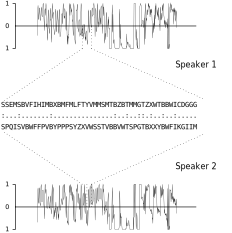
\includegraphics[width=\textwidth]{Body/Images-chap4/voice.pdf}

            %\scalebox{0.80}{
            %   \footnotesize
            %   \psset{xunit=1cm,yunit=1cm}
\readdata{\dataA}{Figures/voiceSeq1-xy.dat}
\readdata{\dataB}{Figures/voiceSeq2-xy.dat}
\begin{pspicture}(0,0)(10,10)%\showgrid
	\rput(2,9){
		\rput(-1,0){
			\psaxes[tickstyle=bottom, dy=\psyunit,Dy=1,Oy=0,Ox=0,Dx=100](0,0)(0,-1)(8,1)
		}
		\dataplot[plotstyle=line,linecolor=black,linewidth=0.1mm]{\dataA}
	}
	\rput(2,1){
		\rput(-1,0){
			\psaxes[tickstyle=bottom, dy=\psyunit,Dy=1,Oy=0,Ox=0,Dx=100](0,0)(0,-1)(8,1)
		}
		\dataplot[plotstyle=line,linecolor=black,linewidth=0.1mm]{\dataB}
	}
	\rput[l](0.4, 5.5){\normalsize \texttt{SSEMSBVFIHIMBXBMFMLFTYVMMSMTBZBTMMGTZXWTBBWICDGGG}}
	\rput[l](0.4, 5){\normalsize \texttt{:...:.......:...............:..:..::.:..:..:.....}}
	\rput[l](0.4, 4.5){\normalsize \texttt{SPQISVBWFFPVBYPPPSYZXVWSSTVBBVWTSPGTBXXYBWFIKGIIM}}
	\rput(0, 0){
		\psline[linestyle=dotted](4,2)(0.55,4.3)
		\psline[linestyle=dotted](4.4,2)(10.6,4.3)
		\psline[linestyle=dotted](4.4,2)(4.4,1)
		\psline[linestyle=dotted](4.2,2)(4.2,1)
	}
	\rput(0, 0){
		\psline[linestyle=dotted](4,8)(0.55,5.7)
		\psline[linestyle=dotted](4.4,8)(10.6,5.7)
		\psline[linestyle=dotted](4,8)(4,9)
		\psline[linestyle=dotted](4.4,8)(4.4,9)
	}
	\rput[bl](8.5, 8){Speaker 1}
	\rput[tl](8.5, 2){Speaker 2}

		
		
%	\rput(0.8,150){
%		\rotatebox{90}{ \# sequences}
%	}
%	\rput(8.5,150){
%		\rotatebox{-90}{ \# patterns}
%	}
%	\rput(5,0){
%		bootstrapping iterations
%	}


%	number LSWBBTTTTYZXBW SSEMSBVFIHIMBXBMFMLFTYVMMSMTBZBTMMGTZXWTBBWICD
%	       .............. :...:.......:...............:..:..::.:..:..:..
%	number TZXYSMFPYVVVTS SPQISVBWFFPVBYPPPSYZXVWSSTVBBVWTSPGTBXXYBWFIKG
%	250       260       270       280       290       300

%	310       320       330       340       350       360
%	number GGGCIWYFMELKKFTKPLILAAAAAAAAAADWZIHWIDDCCDNRAAAAAAAAAAAAAAAA
%	       ....................:::::::::...... ........::::::::::::::::
%	number IIMKPFIILHGDMSYTIEHEAAAAAAAAARITBTDEMGQEHCRAAAAAAAAAAAAAAAAA

\end{pspicture}

            %   \normalsize
            %}
        \caption[A Voice alignment of the spoken--letter ``X'' recorded from two different speakers]{
            An alignment of the spoken--letter ``X'' recorded from two different speakers.
            The plots at the top and bottom are recordings for first and second
            speakers, respectively.  The breakout in the center shows a section of the protein
            projection of each recording and the alignment generated using FastA
            as described in the text.  This example was taken from the first speech
            recognition experiment.  In this case, the bottom recording was the top
            scoring alignment against the top recording.
        }
        \label{fig:voiceAlign}
        \end{figure}

        \begin{figure}[phtb]
        \centering
        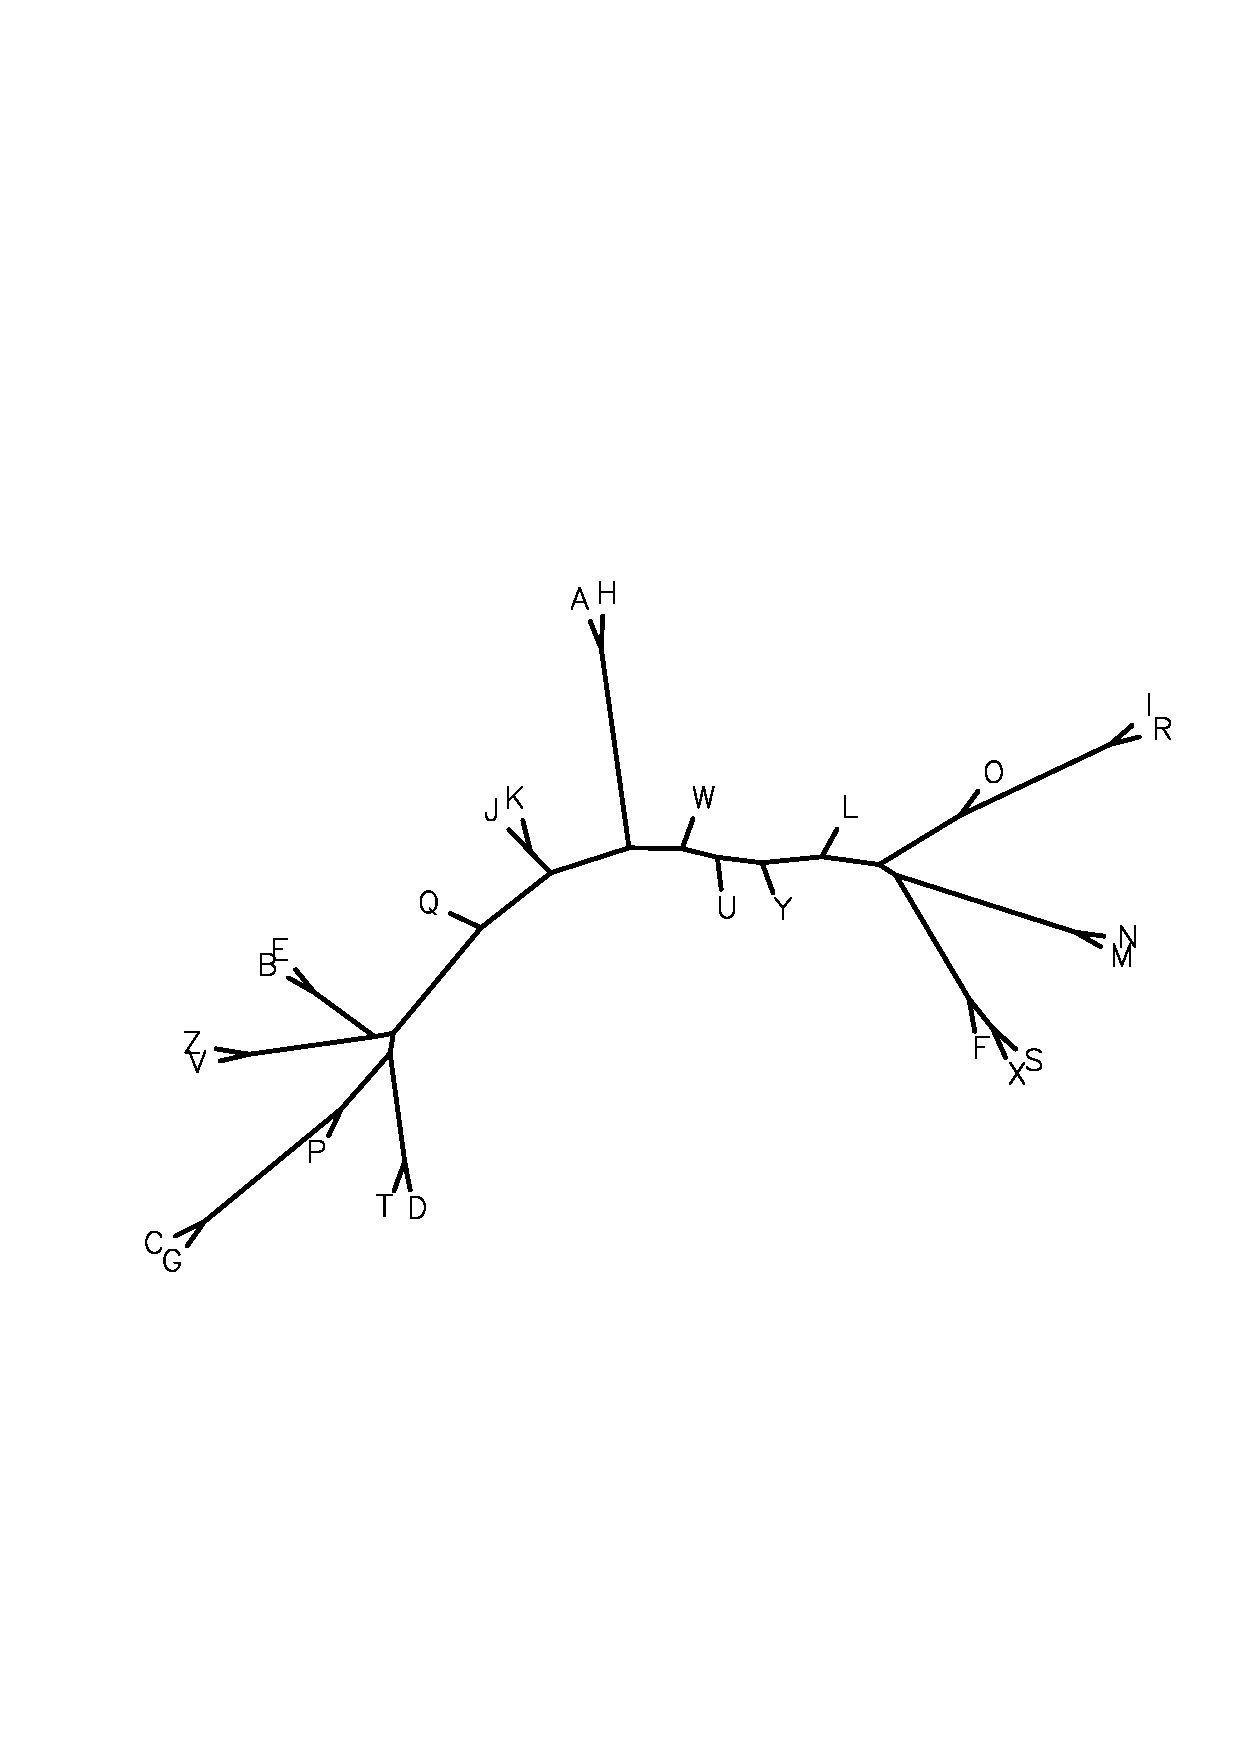
\includegraphics[width=\textwidth]{Body/Images-chap4/tree.pdf}
        \caption[A phylogenetic tree of voice--proteins]{
            A phylogenetic tree of voice--proteins.
            This tree was created using the
            Phylip~\cite{felsenstein1989phylip} tree drawing
            program from a multiple sequence alignment of
            all 26 voice--proteins from a single speaker.
            The multiple sequence alignment was made using the
            ClustalW~\cite{higgins1992improved} alignment tool,
            with the scoring matrix in Table~\vref{table:matrix}.
            In the tree, similar sounding (homologous) letters
            are grouped near each other.  For example, all the
            letters containing the /ee/ sound [\emph{B, C, D,
            E, G, P, T, V, Z}] are clustered on the left side
            of the tree.
        } \label{fig:tree} \end{figure}



\subsection{System and Methods}
    \subsubsection{Handwriting Recognition}
        For our handwriting recognition experiments, we used
        data from Alimoglu and Alpaydin, 1996, available in the
        University of California Irvine repository of machine
        learning databases~\cite{uci1998ucirepository}.  These data
        comprised of 10992 handwritten digits between \emph{0}
        and \emph{9}, written by 44 writers with each writer
        submitting 250 digits (8 samples were discarded by the
        original authors).

        Each digit was written with a stylus pen on a touch tablet,
        which recorded the $x$ and $y$ coordinates of the pen as a
        function of time.  These data were re-sampled such that each
        written digit was represented by a series of eight $(x,y)$
        points, spaced out by a constant arc length over the path of
        the digit.  Then, for each digit, the set of $(x,y)$ points
        were scaled such that the largest axis, usually the $y$ axis,
        ranged from 0 to 1.  By dividing the number line $[0,1]$
        into 23 ``bins'' we translated each of these coordinates
        into a pair of amino acids as shown in Figure~\vref{fig:pda}.
        We concatenated these amino acid pairs to obtain a protein
        sequence representation of each digit: a ``digit--protein.''




    \subsubsection{Speech Recognition}
        For our speech recognition experiments, we used data from
        Deitterich and Bakiri, 1995, %~\cite{dietterich1995solving}
        available in the University of California Irvine repository
        of machine learning databases~\cite{uci1998ucirepository}.
        This data set consisted of 7797 recordings of individuals
        speaking one of the letters \emph{A--Z}.  A total of 150
        speakers each said every letter \emph{A--Z} twice (three
        recordings were discarded by the original authors).
        Then, each recording was processed into a set of 617
        real--valued attributes in the range $[-1,1]$.  A more
        detailed description of the database is available from
        Dietterich \& Bakiri, 1995.%~\cite{dietterich1995solving}.

        By dividing the number line $[-1,1]$ into 23 bins we translated these real numbers into a series
        of amino acids.  For example, the series ``-1.0,-0.55, 0.11, 0.65'' was translated
        to ``{\texttt{AQKY}}''.  We concatenated these amino acids to make a protein representation
        of each recording: a ``voice--protein''.


\subsection{Results}
    \subsubsection{Handwriting Recognition}

        We conducted two handwriting recognition experiments.
        In both experiments part of the digit--protein database was assumed to contain a
        ``known'' set of digits that was subsequently used to annotate,
        or classify, the remaining ``unknown'' digits.  For our
        first experiment, we used for the known database containing the
        writing of 30 persons (7494 digits) and an unknown database
        with the writing of the remaining 14 persons (3498 digits).
        Using FastA, we searched each sequence from the unknown
        set in the known set and used the top scoring hits to
        annotate the unknown digits.  Searches were carried out
        using the scoring matrix shown in Table~\vref{table:matrix}
        with FastA version 3.4t11 using the default gap open and
        extension penalties, and the following options: \texttt{-p
        -Q -d0 -f-8 -g-1 -H -E1000 -b1}.  An example alignment of
        two handwritten nines from different writers is shown in
        Figure~\vref{fig:pdaAlign}.


        For our second experiment, we used 25\% (2748 digits) of our
        digit--protein database, selected randomly, as the unknown
        set and the remaining 75\% (8244 digits) as our known set.
        Alignments and annotations using FastA were performed as
        in the first experiment.

        The results of the two handwriting recognition
        experiments are shown in Table~\vref{table:results1}.
        In experiment 1, our results are about the same as
        the best k--means clustering results of Alimoglu and
        Alpaydin~\cite{alimoglu1996methods,alimoglu1997combining}.
        This experiment simulates the user--independent
        handwriting recognition problem: the handwriting of one
        group of writers was used to classify digits from a different group.
        In the user--dependent problem, experiment 2, the database
        of known handwritten digits contains samples from all the writers,
        on average.  Thus, for every unknown handwriting sample,
        there is often a close match in the database of known
        samples.  As such, the results of experiment 2 are
        significantly better than those of experiment 1 as shown
        in Table~\vref{table:results1}.



        %In contrast to k--means clustering and other common machine learning techniques for handwriting
        %recognition, there was no explicit training or learning phase of our experiments.  As such,
        %we included experiment 3, which is a realistic approximation of the recognition problem
        %on a tablet PC with multiple users.  The results for this experiment are considerably better than
        %experiment 2 because there are relatively more known sequences which can be used for annotating
        %the unknown sequence.

        In experiment 1, the average time for each alignment was
        0.117 seconds per unknown sequence on a 1 gHz Pentium III
        processor.  This is much shorter than the time required to
        write the digits.  Thus sequence alignment could be used
        as a ``real--time'' method for handwriting recognition.
        This high speed, together with the high accuracy for
        user--dependent recognition makes sequence alignment good
        candidate for use on a Tablet PCs, or even PDAs.

    \subsubsection{Speech Recognition}


        Using the voice--protein database, we conducted two
        experiments, analogous to the two handwriting recognition
        experiments described previously.  First, we used a known
        set consisting of 6238 recordings from 120 speakers and
        an unknown set with 1559 recordings from the remaining 30
        speakers.  Second, we used 25\% (1949 recordings) of the
        voice--protein database, selected randomly, as the unknown
        set and the remaining 75\% (5848 recordings) as the known
        set.  Each of the speech recognition alignments was performed
        using the same scoring matrix and FastA parameters as the
        handwriting recognition experiments.  An example alignment
        of two voice--proteins is shown in Figure~\vref{fig:voiceAlign}.


        The results of the two speech recognition experiments are shown in
        Table~\vref{table:results2}.
        Experiment 1 is compared
        to the best Error Correcting Output Code (ECOC) results of Deitterich
        and Bakiri~\cite{dietterich1995solving},
        but
        there was no comparison available for experiment 2.
        The misclassification for experiment 1 was 6.16\%,
        higher than the ECOC result of 3.27\%.  However, we observed that
        most of the errors were due to rhyming letters, and in particular
        all of the /ee/ sounding characters [\emph{B, C, D, E, G, P, T, V, Z}].
        This indicated that these characters were similar on a sequence level,
        so we constructed a phylogenetic tree of the sequences to study their
        relationship.



        A phylogenetic tree of 26 voice--proteins from a single
        speaker is shown in Figure~\vref{fig:tree}.  As the figure
        shows, the protein projections of phonetically similar
        letters tend to be homologous.  Furthermore, letters such
        as \emph{A} and \emph{H}, which have the /ay/ sound at the
        beginning, are more closely related to each other than
        they are to \emph{J} and \emph{K}, which have the /ay/
        sound at the end.  Because the /ee/ sounding letters all
        have /ee/ at the end, they are particularly difficult
        to distinguish from each other.  These letters account
        for a disproportionate majority of the errors in our two
        experiments.  By clustering these letters together such that
        they are considered the same for classification purposes,
        the error in experiment 1 was reduced to 1.09\%.  If the
        original error was evenly distributed between the classes,
        the error would have been reduced only to about 5.5\%.
        This suggests that, although string alignment performs
        poorly for /ee/ sounding characters, it performs well for
        all other characters.


\subsection{Conclusions}
        This work showed that sequence alignment can be a powerful
        classification tool for problems outside the domain
        of bioinformatics.  In both the handwriting and speech
        recognition problems, we projected real--valued data into
        strings of amino acids and used FastA as a classification
        tool, in a manner analogous to protein annotation.  In the
        case of handwriting recognition, we showed that sequence
        alignment is a viable alternative to traditional methods,
        such as k--means clustering, and is fast enough to be used
        as a real--time recognition method.


        There are many ways to improve upon the results we presented here.
        First, we did not have any explicit training phase for either set of experiments.
        However, there are at least two sequence alignment parameters which can
        be trained: the gap open and extension penalties, and the scoring matrix.
        The optimization of these parameters for protein annotation is well documented
        ~\cite{henikoff1993performance,altschul1991amino,henikoff1992aminoacid,dayhoff1979amodel,vogt1995assessment,henikoff2000amino}
        and would be similar for alternative sequence alignment applications such
        as handwriting recognition.  Second, intelligent projection of data
        into strings can greatly improve results.  Here, we used bins of equal
        size to partition the real--valued data into amino acids; however, bins
        of unequal size may improve the resolution between closely related sequences
        and improve classification.  Finally, more customizable sequence alignment tools
        would be very useful.  These tools should take an arbitrary alphabet (Blast
        and FastA are restricted to 23 amino acids) and a user--defined scoring
        matrix (FastA allows user--defined matrices, but Blast does not).

        The potential applications of sequence alignment tools
        outside of bioinformatics are boundless.  Tools such as Blast
        and FastA can be used to quickly classify or search through
        any data that can be projected into a string of characters.
        Of course, these methods will work best with data that is
        of a low dimension.  Our experiments with more complex data
        data, such as color images, suggest that how the data are
        projected into a string is very important with large number
        of dimensions.  However, for simple types of data, such
        as customer purchase histories, black and white images, or
        Internet chat transcripts, we have been able to use sequence
        alignment as a quick and effective classification tool.

\clearpage
\section{Machine learning approaches to modeling the physiochemical properties of
peptides}

% The very first letter is a 2 line initial drop letter followed
% by the rest of the first word in caps.
%
% form to use if the first word consists of a single letter:
% \PARstart{A}{demo} file is ....
%
% form to use if you need the single drop letter followed by
% normal text (unknown if ever used by IEEE):
% \PARstart{A}{}demo file is ....
%
% Some journals put the first two words in caps:
% \PARstart{T}{his demo} file is ....
%
% Here we have the typical use of a "T" for an initial drop letter
% and "HIS" in caps to complete the first word.
\subsection{Introduction}
In this section, I discuss the modeling of small peptide sequences
using non--grammatical models. Most commonly, peptides and protein
sequences are represented as a string of letters drawn from the
alphabet of characters representing the twenty natural amino acids.
Here, I present a series of experiments using a more meaningful
representation of amino acids and test the ability of various
machine learning techniques to predict peptide function.
Specifically, I develop a set of three amino acid representation
schemes and test these schemes combinatorially with a set of six
machine learning techniques. All of the work described in this
section
    is part of a publication appearing in the proceedings of the fourth
    Singapore--MIT Alliance Programme on Molecular Engineering of Biological and Chemical
    Systems, which was co--authored with Mark Styczynski and Gregory Stephanopoulos.
    Throughout this section, the use of the pronoun ``we'' refers to
    these authors.

\subsection{Motivation and background}

\subsubsection{Amino acid representations}
The most common representation of small peptides are as strings of
letters representing the twenty amino acids, e.g. \texttt{KWRAG},
which is the five residue sequence lysine, tryptophan, arginine,
alanine, and glycine.  Notably, both amino acid names and their
corresponding abbreviations are human constructs that carry no
information about the underlying physiochemical characteristics of
each amino acid.  That is, the string \texttt{KWRAG} carries little
information in and of itself, without some information about what a
\texttt{K} is and how it is different from the other amino acids.
In place of such physical descriptions, previous efforts have
described the similarity of amino acids based on the tendency for
one amino acid to substitute for another in homologous,
similarly--functioning proteins across different
species~\cite{henikoff1992aminoacid,dayhoff1979amodel}. That is,
substitutions that are observed in nature can be construed in some
sense as indicating similarity between certain amino acids. While
such efforts have been extremely useful for tasks such as aligning
more distant protein homologs, they typically do not capture enough
information to be practically useful in \textit{de novo} design or
prediction of protein activity.

Here we experiment with feature vector representations of small
peptides using sets of amino acid physiochemical characteristics
derived from the AAindex
database~\cite{kawashima1999aaindex,tomii1996analysis,nakai1988cluster}.
The AAindex database lists 453 physiochemical parameters for each of
the twenty amino acids.  These parameters range from those that are
very tangible and intuitive --- for example, residue volume, which
is AAindex parameter BIGC670101~\cite{bigelow1967on} --- to the
abstract --- for example, the normalized frequency of participation
in an N-terminal beta--sheet, which is AAindex parameter
CHOP780208~\cite{chou1978prediction}.  The parameters were culled
from the scientific literature by the AAindex authors and might be
considered the universe of what we, as the scientific community,
know about each amino acid.

Thus, a very logical way of representing an amino acid is as a
feature vector of these 453 attributes.  In this sense each type of
amino acid has a different feature vector of the same
dimensionality.  This might be considered the ``maximally
informative'' representation of the amino acids since it
incorporates an expansive set of features culled from the
literature.  Extending this, we could write an amino acid sequence
as the concatenation of these vectors.  That is, a three residue
peptide could be represented as a $3*453=1359$ feature vector.
Intuitively, this representation retains more information than the
string representation.  Further, we would imagine that the
physiochemical representation would be more useful for modeling the
function of a peptide sequence, such as its propensity to fold in a
certain manner or to react with a certain enzyme.

The representation of amino acids has received some previous
attention in the literature.  For example, Atchley \emph{et.\
al.}~\cite{atchley2005solving} use the physiochemical parameters
from the AAindex to create a low--dimensional projection of the
characteristics of each of the twenty natural amino acids.  Further,
they used this low--dimensional progression to derive metrics of
similarity between the amino acids, similar to popular amino acid
scoring matrices such as Blosum~\cite{henikoff1992aminoacid} and
PAM~\cite{dayhoff1979amodel}.


%\cite{buck2005networks}
%\cite{grantham1974amino}
% needed in second column of first page if using \pubid
%\pubidadjcol

\subsubsection{HIV--I Protease}
In this work we will use the HIV--I protease as a model system for
demonstrating the merits of different physiochemical amino acid
representations.  Specifically, we show the success of different
representations and different machine learning methods at modeling
substrate specificity of the protease.

The HIV--1 protease is a proteolytic enzyme encoded by the HIV
genome~\cite{brik2003hiv}.  The protease plays a critical role in
viral replication and the development of viral
structure~\cite{wang2001computational}. The protease recognizes
specific eight--residue sequences in its substrates (see
Figures~\vref{fig:hiv1p} and~\vref{fig:pockets}).  The protease's
natural targets are subsequences of other HIV genes which must be
cleaved for the virus to successfully replicate.  Accordingly, small
molecule inhibitors of the protease are a common therapy for
HIV/AIDS~\cite{boden1998resistance}.

    \begin{figure}[phbt]
    \centering
    \includegraphics[width=2.5in]{Body/Images-chap4/hiv1p.png}
    \caption[Structure of the HIV--I protease,
    derived from the Protein Data Bank
    (PDB)~\cite{berman2000protein} entry 7HVP~\cite{swain1990x-ray}]{Structure of the HIV--I protease,
    derived from the Protein Data Bank
    (PDB)~\cite{berman2000protein} entry 7HVP~\cite{swain1990x-ray}.
    Over one hundred other structures of the protease
    have been solved since the first in 1989 and are
    available from the PDB's website.  The protein is
    a dimer of two 99 amino acid chains.  The regions
    of the protein at the top of the figure, the
    ``flaps,'' open up and accept a substrate protein,
    closing behind it.  Two aspartate residues in the
    active site, aided by the presence of water,
    act to cleave the substrate.} \label{fig:hiv1p}
    \end{figure}

    \begin{figure}[phbt]
    \centering
    \includegraphics[width=2.0in]{Body/Images-chap4/pockets.png}
    \caption[Schematic of the HIV--I protease active site]{Schematic of the HIV--I protease active site.
    The active site comprises eight binding pockets (P1--P4
    and P1'--P4') into which eight residues from the
    target protein fall.  The target protein is cleaved between
    the S1 and S1' residues.  One half of the catalytic
    unit is made up by chain A of the protease and the
    other by chain B (see Figure~\vref{fig:hiv1p}).
    }
    \label{fig:pockets}
    \end{figure}

In addition to the handful of sites that the protease cleaves to
facilitate viral development, it can cleave a number of other
``non--natural'' substrates~\cite{beck2002defining}.  These
substrates have been the focus of intense experimental
study~\cite{beck2000identification,bagossi2005amino,beck2001molecular,
clemente2004comparing}.  In a recent manuscript, You \emph{et.\
al.}\ collected a comprehensive set of 700+ eight--residue
substrates that have been tested for cleavability by the HIV--I
protease~\cite{you2005comprehensive}.  In addition, You \emph{et.\
al.}\ developed a series of models for the protease's substrate
selectivity that, in general, outperform previous computational
models~\cite{cai2002support,chou1996prediction,narayanan2002mining,rognvaldsson2004why},
which relied on a much smaller dataset~\cite{cai1998artificial}.


%\cite{brown2000knowledge-based}
%\cite{callebaut1996inhibition}


\subsection{Methods}

\subsubsection{Amino acid representations and input
data set} A set of 746 eight--residue peptides were generously
provided by You \emph{et. al.}\ ~\cite{you2005comprehensive}, each
with a class: cleavable by the HIV--I protease or not cleavable.  In
addition, the complete set of 453 physiochemical parameters for each
of the 20 naturally occurring amino acids was downloaded from the
AAindex database (release 7.0, July 2005).

From these 453 parameters, we removed redundant parameters for which
the magnitude of the correlation coefficient with another parameter
was greater than 0.80. The remaining 155 independent parameters were
kept.  Using these parameters, we made three different projections
of the 746 experimentally tested protease substrates as detailed
below.

\paragraph{Full physiochemical projection}
In this projection each eight--residue peptide was represented as a
1241--dimensional feature vector: 8 residues with 155 physiochemical
features per residue plus the class --- cleaved or not cleaved.  Of
our three representations, this one retains the most information
about the peptides.

\paragraph{Feature--selected physiochemical projection}
Using the ``FULL'' projection (above) we performed a feature
selection routine to select only those features that are most
correlated to the class.  (Throughout this manuscript, all modeling
and feature selection were performed using the Waikato Environment
for Knowledge Analysis, or WEKA ~\cite{witten2005data}).  Briefly,
we evaluated the worth of a subset of features by considering the
individual predictive ability of each feature with respect to the
cleaved/uncleaved class, along with the degree of redundancy between
the features.  Using this method, we created a 54--dimensional
projection of the peptide substrates (53 features plus the class).

Analysis of this lower--dimensional projection revealed that the
features of the outer residues (S4, S4') are relatively unimportant,
whereas the central residues (S1, S1') are quite important in
determining cleavability. For the S1 position, seven parameters were
chosen:
\begin{itemize}
    \item   FASG760102: Melting point~\cite{fasman1976handbook};
    \item   FAUJ880105: Minimum width of the side
        chain~\cite{fauchere1988amino};

    \item   PALJ810111: Normalized frequency of beta--sheet
        in alpha+beta class~\cite{palau1982protein};

    \item   PRAM900101: Hydrophobicity~\cite{prabhakaran1990distribution};

    \item   ROBB760107: Information measure for
        extended without H-bond~\cite{robson1976conformational};

    \item   KOEP990101: Alpha--helix propensity derived
        from designed sequences~\cite{koehl1999structure-based}; and

    \item   MITS020101: Amphiphilicity
        index~\cite{mitaku2002amphiphilicity}.
\end{itemize}

\paragraph{PCA projection of physiochemical properties}
Using the full, 155--dimensional representation of each of the 20
naturally occurring amino acids, we performed principal component
analysis (PCA) to find linear combinations of features that capture
the variation between different kinds of amino acids.  More
formally, PCA, or the Karhunen--Lo\`{e}ve transform, is a linear
transformation by which the 20 data points in a 155--dimensional
space are projected onto a new coordinate system.  The system is
chosen such that the greatest variance is captured by the first
axis, or the first ``principal component.''  Successive principal
components (axes) capture progressively less variance.  Each
component is a linear combination of some of the initial features;
given appropriate uniform normalization, the weight of each feature
in a given component indicates the relative importance of that
feature in defining the component.

Using PCA, we derived 16 principal components that capture 95\% of
the variance in the amino acids, with the first PC capturing 30\% of
the variance.  The set of 746 peptide 8--mers were projected into a
reduced 129--dimensional space: 8 concatenated 16--dimensional
residues plus the class of the peptide.


\subsubsection{Model creation and classification}
For each of the three peptide representations detailed above, we
tested the ability of six machine learning techniques to classify
the peptides as either cleaved or uncleaved.  Each of these models
is described below. For each model, we evaluated the performance
using 10x10 cross--validation (see Conclusion): for each of ten
runs, 10\% of the peptide dataset was withheld for testing a
classifier trained by the remaining 90\% of the peptides. The
sensitivity and specificity of each classifier's predictions for all
ten of its cross--validation runs can then be combined to determine
the percentage of correctly classified peptides.  This value is used
to quantify the classifier's overall accuracy and facilitates
pairwise comparison of models and representation schemes.

\paragraph{Decision tree model}
Decision trees are simple, intuitive classification schemes that use
a series of questions (decisions) to place a sample in a class with
low error rate. More specifically, a decision tree is a structure in
which the internal branches represent conditions, such as
``hydrophobicity index at S3 $> 0.52$''.  Following these conditions
leads to the leaves of the tree, which are classifications
indicating whether the peptide is cleaved or not.  Here, we use a
particular variant of the decision tree, a C4.5 decision
tree~\cite{quinlan1992c4}, which is notable for not being prone to
overfitting of input data.  An example decision tree from our
experiments is shown in Figure~\vref{fig:decisionTree}.

   \begin{figure}[!h]
    \centering
    %\includegraphics[width=2.5in]{Images/barChart.pdf}
    \tiny
    \begin{verbatim}
CHOP780207_S2' <= 0.41765
|   FAUJ880105_S1 <= 0.57778
|   |   FASG760102_S1 <= 0.27711: uncleaved (32.0/1.0)
|   |   FASG760102_S1 > 0.27711
|   |   |   QIAN880122_S4' <= 0.81022
|   |   |   |   PRAM900101_S1 <= 0.27463
|   |   |   |   |   MEEJ810102_S4 <= 0.33702
|   |   |   |   |   |   RACS820112_S2 <= 0.58621
|   |   |   |   |   |   |   ZIMJ680101_S1' <= 0.52117
|   |   |   |   |   |   |   |   PRAM820101_S2' <= 0.43367
|   |   |   |   |   |   |   |   |   ROSM880103_S3' <= 0.23077: cleaved (2.0)
|   |   |   |   |   |   |   |   |   ROSM880103_S3' > 0.23077
|   |   |   |   |   |   |   |   |   |   CHOP780207_S4 <= 0.21176: cleaved (2.0)
|   |   |   |   |   |   |   |   |   |   CHOP780207_S4 > 0.21176: uncleaved (11.0/1.0)
|   |   |   |   |   |   |   |   PRAM820101_S2' > 0.43367
|   |   |   |   |   |   |   |   |   RADA880105_S2 <= 0.75274
|   |   |   |   |   |   |   |   |   |   PRAM900101_S1 <= 0.06866: cleaved (10.0/2.0)
|   |   |   |   |   |   |   |   |   |   PRAM900101_S1 > 0.06866: uncleaved (4.0)
|   |   |   |   |   |   |   |   |   RADA880105_S2 > 0.75274
|   |   |   |   |   |   |   |   |   |   QIAN880137_S3' <= 0.5124: cleaved (69.0/3.0)
|   |   |   |   |   |   |   |   |   |   QIAN880137_S3' > 0.5124
|   |   |   |   |   |   |   |   |   |   |   RACS820112_S2 <= 0.43103: cleaved (2.0)
|   |   |   |   |   |   |   |   |   |   |   RACS820112_S2 > 0.43103: uncleaved (4.0/1.0)
|   |   |   |   |   |   |   ZIMJ680101_S1' > 0.52117: cleaved (248.0/7.0)
|   |   |   |   |   |   RACS820112_S2 > 0.58621
|   |   |   |   |   |   |   RACS820103_S4 <= 0.43007
|   |   |   |   |   |   |   |   CHAM830104_S3' <= 0
|   |   |   |   |   |   |   |   |   RADA880105_S2 <= 0.75274: uncleaved (5.0/1.0)
|   |   |   |   |   |   |   |   |   RADA880105_S2 > 0.75274: cleaved (2.0)
|   |   |   |   |   |   |   |   CHAM830104_S3' > 0: cleaved (11.0)
|   |   |   |   |   |   |   RACS820103_S4 > 0.43007: uncleaved (6.0)
|   |   |   |   |   MEEJ810102_S4 > 0.33702
|   |   |   |   |   |   GARJ730101_S4' <= 0.01426: uncleaved (9.0)
|   |   |   |   |   |   GARJ730101_S4' > 0.01426
|   |   |   |   |   |   |   CHAM830104_S3' <= 0
|   |   |   |   |   |   |   |   QIAN880102_S4 <= 0.57143: uncleaved (7.0/1.0)
|   |   |   |   |   |   |   |   QIAN880102_S4 > 0.57143: cleaved (3.0)
|   |   |   |   |   |   |   CHAM830104_S3' > 0: cleaved (9.0)
|   |   |   |   PRAM900101_S1 > 0.27463
|   |   |   |   |   GEIM800106_S1' <= 0.94
|   |   |   |   |   |   RACS820102_S3 <= 0.81522
|   |   |   |   |   |   |   FAUJ880108_S2' <= 0.4375: uncleaved (31.0/1.0)
|   |   |   |   |   |   |   FAUJ880108_S2' > 0.4375: cleaved (4.0/1.0)
|   |   |   |   |   |   RACS820102_S3 > 0.81522: cleaved (6.0)
|   |   |   |   |   GEIM800106_S1' > 0.94: cleaved (9.0)
|   |   |   QIAN880122_S4' > 0.81022
|   |   |   |   MITS020101_S1 <= 0.35354
|   |   |   |   |   ZIMJ680101_S1' <= 0.82085: uncleaved (20.0)
|   |   |   |   |   ZIMJ680101_S1' > 0.82085
|   |   |   |   |   |   RACS820102_S3 <= 0.3587: uncleaved (4.0)
|   |   |   |   |   |   RACS820102_S3 > 0.3587: cleaved (5.0)
|   |   |   |   MITS020101_S1 > 0.35354: cleaved (2.0)
|   FAUJ880105_S1 > 0.57778
|   |   QIAN880137_S3' <= 0: cleaved (3.0)
|   |   QIAN880137_S3' > 0: uncleaved (37.0/1.0)
CHOP780207_S2' > 0.41765
|   ZIMJ680101_S1' <= 0.58306: uncleaved (145.0/2.0)
|   ZIMJ680101_S1' > 0.58306
|   |   PRAM900101_S1 <= 0.27463
|   |   |   FAUJ880105_S1 <= 0.57778
|   |   |   |   FAUJ880105_S1 <= 0: uncleaved (2.0)
|   |   |   |   FAUJ880105_S1 > 0
|   |   |   |   |   RACS820103_S3 <= 0.72378
|   |   |   |   |   |   WILM950104_S2 <= 0.44834: uncleaved (5.0)
|   |   |   |   |   |   WILM950104_S2 > 0.44834
|   |   |   |   |   |   |   PRAM820101_S2' <= 0.77041: cleaved (8.0)
|   |   |   |   |   |   |   PRAM820101_S2' > 0.77041: uncleaved (4.0/1.0)
|   |   |   |   |   RACS820103_S3 > 0.72378: cleaved (9.0)
|   |   |   FAUJ880105_S1 > 0.57778: uncleaved (4.0)
|   |   PRAM900101_S1 > 0.27463: uncleaved (12.0)
    \end{verbatim}
    \caption[Decision tree calculated for modeling 8--mer peptides]{The decision tree calculated for the
    CFS, a 54--dimensional representation of the 8--mer
    peptides.  The branch points are in the form
    PARAMETER\_RESIDUE\@.  For example, \texttt{CHOP780207\_S2'}
    represents the AAindex parameter \texttt{CHOP780207}
    (normalized frequency of participation in a C--terminal non--helical
    region) at the S2' residue.  Values for all
    AAindex parameters are normalized to 1 across all
    amino acids.  The tree shows various questions
    about a peptide that, when followed, lead to a
    set of conclusions.   For example, if 
    a given peptide has
    \texttt{CHOP780207\_S2 <= 0.41765} and
    \texttt{FAUJ880105\_S1 > 0.57778} and
    \texttt{QIAN880137\_S3 > 0} then the peptide
    is classified as uncleaved.  As shown in the
    table, 37 of the 746 known peptides are
    correctly classified
    by this scheme and only one is incorrectly
    classified.
    } \label{fig:decisionTree}
    \end{figure}


\paragraph{Logistic regression model}
A logistic regression is just a non--linear transformation of a
linear regression.  In this model, each independent variable (the
different dimensions of our various projections) are regressed to
the class (cleaved or not cleaved).  Here we use a variant of
logistic regression that leads to automated feature selection and is
described elsewhere~\cite{landwehr2003logistic}.

\paragraph{Bayesian network model}
Bayesian network models use directed acyclic graphs to model the
joint probability distribution of each class over all input
features. That is, the model captures conditional dependencies
between the features with regards to how they impact the final
classification of each sample.  Bayesian networks can be used to
find causality relationships, one of many features that make these
models particularly well--suited to many applications in
computational biology (see, for
example,~\cite{scott2004predicting,hartemink2002bayesian,friedman2000using}).
The method uses a Bayesian scoring metric that ranks multiple models
based on their ability to explain data with the simplest possible
method.  The Bayesian metric is a function of the probability of the
model being correct given a set of observed data; this is, in turn,
correlated to the model's prior probability and its physical
likelihood. For a more detailed explanation of Bayesian networks,
see Witten and Frank~\cite{witten2005data} or
Heckerman~\cite{heckerman95tutorial}.

\paragraph{Naive Bayes model} The naive Bayes model, or ``Idiot's''
Bayes model~\cite{hand2001idiots}, is a simple machine learning
scheme that assumes \emph{naively} that each feature has an
independent effect on the classification of each
sample~\cite{john1995estimating}.  In the case of the HIV--I
protease substrates, this means that the physiochemical
characteristics of the S1 residue contribute to the cleavability of
the peptide in a way that is independent of the other residues: S1',
S2, etc.  The resulting network dependencies are less complex than
one might otherwise obtain from a Bayesian network model but are
frequently useful, particularly for unwieldy datasets or problems
with physical characteristics that may warrant the assumption of
conditional independence of features.

\paragraph{Support vector machine model with linear basis function}
The support vector machine (SVM) is a machine learning technique
posed as a quadratic programming (QP)
problem~\cite{bennett2000support}. The formulation can best be
conceptualized by considering the problem of classifying two
linearly separable groups of points.  The first step is to define
the ``convex hull'' of each group, which is the smallest--area
convex polygon that completely contains a group.  The SVM approach
looks for the best linear classifier (single straight line) between
the two groups of points, defined as either the line that bisects
the two closest points on each convex hull or the two parallel
planes tangent to each convex hull that are furthest apart.  These
alternative definitions provide two alternative formulations of a
convex QP problem; notably, they both reduce to the same problem.
(A rigorous mathematical treatment of these qualitative explanations
can be found
elsewhere~\cite{bennett2000duality,crisp1999geometric}.) Tried and
true methods for solving QP problems can then be used to (relatively
quickly) determine the best classifier.  This method can be expanded
to allow for linearly inseparable cases by altering the optimization
problem to account for a weighted cost of misclassification when
training the model.  There is evidence in the literature that an SVM
approach to defining the best classifier is less susceptible to
overfitting and generalization
error~\cite{cristianini2000introduction,vapnik1998statistical,vapnik1995nature}.

\paragraph{Support vector machine model with radial basis function}
The above description of an SVM, despite accounting for the
possibility of inseparability, does not address the need for
non--linear classifiers. For instance, if the members of one class
fall within a well--defined circle and the non--members fall outside
of the circle, the above method will perform extremely poorly
because it will try to form just one plane to separate the
groups~\cite{bennett2000support}.  Rather than attempting to fit
higher--order curves, it is easier to project the input attributes
into a higher--dimensional space in which the groups are
(approximately) linearly separable.  The higher--dimensional spaces
can be characteristic of any desired classifier (e.g., nonlinear
terms generated by multiplying attributes or squaring attributes).
The same method for computing the best linear classifier is then
used.   The result is mapped back into attribute space of the
appropriate dimensions and constitutes a non--linear classifier.
Though one may expect such a process to be prohibitively expensive
for data with many attributes, there exists a computational shortcut
using ``kernel functions'' to avoid calculating all possible
higher--dimensional feature values.  In this work, the basis
function for the kernel gives us the ability to detect optimal
classifiers that are based upon training points' radius from some
center point (as in the above example).



\subsection{Conclusion}
    Our results show that the full, 1241--dimensional
    representation performed the best, followed by the PCA
    representation and, finally, the representation made
    via feature selection.  (See Figure~\vref{fig:barChart}
    and Table~\vref{table:repComp} \&~\vref{table:repRank}.
    In these tables ``FULL'' is the full physiochemical,
    1241--dimensional representation; ``CFS'' is the
    feature--selected, 55--dimensional representation; and
    ``PCA'' is the 129--dimensional representation
    created using principal component analysis.)

    \begin{figure}[phbt]
    \centering
    \includegraphics[width=2.5in]{Body/Images-chap4/barChart.pdf}
    \caption[Classification results for all
    amino acid representations and model types]{Classification results for all
    amino acid representations and model types.
    The three different amino acid representations
    are shown in shades of gray: ``FULL'' is the full
    physiochemical, 1241--dimensional representation;
    ``CFS'' is the feature--selected, 55--dimensional
    representation; and ``PCA'' is the 129--dimensional
    representation using created using princple
    component analysis (see text).  Error bars
    show the standard deviation over the
    10x10 cross--validation test (100 samples per
    representation/model combination with a total of
    1800 tests.)  The best performing model was the
    SVM with radial basis function (SVM--rbf in the
    figure) with the full 1241--dimensional feature
    vector representing each eight--residue sequence.
    Averaged over all representations, the logistic
    regression model is best (see Table~\vref{table:modelComp}).
    The poorest performing model is the decision tree
    (DT) with the 129--dimensional feature vector
    created using the PCA projections created as
    described in the text.  In general the full 1241--dimensional
    representation performed the best,
    followed by the PCA representation and finally
    the CFS representation, which was created by a
    feature selection process.  } \label{fig:barChart}
    \end{figure}

    Of the models tested, results show that logistic
    regression is the best, followed by (linear basis function) SVMs and
    Bayesian networks (See Figure~\vref{fig:barChart} and
    Table~\vref{table:modelComp} \&~\vref{table:modelRank}.)  The
    single best model/representation combination was the
    SVM model with radial basis function (SVM--rbf) and
    the FULL representation.  It is worth noting that though
    this single combination was the best, the radial basis function
    SVM itself did not perform consistently well.  Though this
    may not have been expected, it is definitely reasonable
    per the ``No Free Lunch'' theorem:
    no single machine--learning method should be expected to
    perform the best in all cases~\cite{wolpert1995no}.

    In general, these results suggest that
    higher--dimensional physiochemical representations
    tend to have better performance than representations
    incorporating fewer dimensions selected on the basis
    of high information content.  As such, it seems that
    as long as the training set is a reasonable
    size, more accurate classifiers can be constructed by
    keeping as many significant input attributes as possible.
    Though methods like principal
    components analysis help to reduce computational complexity
    for unwieldy datasets, it is better to avoid feature
    selection until a supervised method (like the models tested
    in this work) can determine which features are most important
    in classifying samples.

    \begin{table}
    \caption[Machine learning model comparison]{Machine learning model comparison.  Each $i,j$ entry represents the number of representations,
    out of three, for which the $i$ model performed \emph{worse} than the $j$
    model.  Here ``worse'' means that the model had a statistically significant
    lower performance, based on a two--tailed t--test at the 0.05 confidence level.}
    \label{table:modelComp}
    \centering
    \begin{tabular}{rcccccc} \hline \hline
        & DT & LR & NB & BN & SVM & SVM--rbf \\
        DT & - & 2 & 1 & 3 & 2 & 2 \\
        LR & 0 & - & 0 & 0 & 0 & 0 \\
        NB & 0 & 3 & - & 1 & 2 & 1 \\
        BN & 0 & 1 & 0 & - & 1 & 1 \\
        SVM & 0 & 0 & 0 & 0 & - & 1 \\
        SVM--rbf & 0 & 2 & 0 & 1 & 2 & - \\ \hline \hline
    \end{tabular}
    \vspace{12pt}


    \end{table}

    \begin{table}
    \caption[Machine learning model ranking]{Machine learning model ranking. Each row shows,
    for each model, how many other model/representation
    pairs that model (with any
    representation) ``wins'' against.  (Thus, the max of the sum
    of the columns in any row is $18-3=15$; however,
    ties are not shown.)  Here ``win/loss'' means
    that the model had a statistically significant
    higher/lower performance, based on a two--tailed
    t--test at the 0.05 confidence level.}\label{table:modelRank}
    \centering
    \begin{tabular}{ccc} \hline \hline
        total wins & total losses & model \\ \hline
       8 &  0 &  LR \\
       7 &  1 &  SVM \\
       5 &  3 &  BN \\
       5 &  5 &  SVM--rbf \\
       1 &  7 &  NB \\
       0 &  10 &  DT \\ \hline \hline
    \end{tabular}
    \vspace{12pt}
    \end{table}

    \begin{table}
    \caption[Machine learning representation comparison]    {Machine learning representation comparison.  Each $i,j$ entry represents the
    number of models, out of six, for which the $i$
    representation performed \emph{worse} than the
    $j$ representation.  Here ``worse'' means that
    the representation had a statistically significant
    lower performance, based on a two--tailed t--test
    at the 0.05 confidence level.}\label{table:repComp}
    \centering
    \begin{tabular}{rccc} \hline \hline
    & FULL & CFS & PCA \\
     FULL & - & 0 & 1  \\
     CFS & 3 & - & 4  \\
     PCA & 2 & 1 & -  \\ \hline \hline
    \end{tabular}
    \vspace{12pt}
    \end{table}

    \begin{table}
    \caption[Machine learning representation ranking]{Machine learning representation ranking. Each row shows, for each representation,
    how many other model/representation pairs that representation (with any
    model) ``wins'' against.  (Thus, the max of the sum
    of the columns in any row is $18-6=12$; however,
    ties are not shown.)  Here ``win/loss'' means
    that the representation had a statistically significant
    higher/lower performance, based on a two--tailed
    t--test at the 0.05 confidence level.}\label{table:repRank}
    \centering
    \begin{tabular}{ccc} \hline \hline
    5 & 1 & FULL \\
    5 & 3 & PCA \\
    1 & 7 & CFS \\ \hline
    \end{tabular}
    \vspace{12pt}

    \end{table}

\clearpage
\section{Identifying functionally important mutations from phenotypically diverse sequence data}
\subsection{Introduction}

In the previous section, I departed from the use of grammar--based
models of sequences and explored statistical modeling approaches.
This section continues this line of work, but is focused on the
identification of important mutations in nucleotide sequences,
rather than global, physiochemical characteristics of small
peptides.  In particular, in this section I present a simple
statistical method for parsing out the phenotypic contribution of a
single mutation from libraries of functional diversity that contain
a multitude of mutations and varied phenotypes. This work is part of
a publication that is in press at \emph{Applied and Environmental
Microbiology}, which was co--authored with Hal Alper, Curt Fischer,
and Gregory Stephanopoulos.  Throughout this section, the use of the
pronoun ``we'' refers to these authors.


\subsection{Motivation}

    The engineering of  functional nucleic acid sequences
    and other biomolecules is frequently hampered by a
    limited understanding of how specific mutations at
    a genotype level are manifested in the phenotype.
    For some well--studied, large protein families, these
    relationships can be inferred; however, such cases
    are rare.  In the absence of these relationships, we
    resort to strategies that explore the genotype space
    in a random manner, such as directed evolution.

    In many cases, directed evolution of genes
    and other functional DNA loci is an effective
    approach to sample the sequence space in search of
    biomolecules with desirable properties ~\cite{glieder2002laboratory,solem2002modulation}.
    However,  the most successful examples employ
    a selectable fitness criterion that allows for
    high-throughput screening of the mutational space:
    sampling a large enough space eliminates the need
    to make rational mutations.  For many proteins or
    functional nucleic acids, it may not be possible
    to link a desired phenotype with a selectable
    criterion, fit for high-throughput screening.
    In the absence of such a criterion, clonal
    populations of mutants must be assayed individually
    for the phenotype of interest.  This scenario
    might be called ``assay--based'' directed evolution,
    a situation in which the upstream mutagenesis
    has a higher throughput than the downstream
    characterization.  In this scenario, there is a
    premium on information linking mutational changes
    to their phenotypic manifestations.  Further,
    there is a strong incentive to ``learn from''
    the  (relatively small) mutational spectra of
    these mutants to determine sequence-phenotype
    interactions, and to use this information
    rationally in subsequent rounds of mutagenesis.

          Here, we present a simple statistical
          method for analyzing a mutational spectrum
          to parse out the phenotypic manifestation
          of individual mutations, even when they
          are masked by the presence of many other
          mutations.  Because assay-based directed
          evolution does not employ any pre--screening
          or selection of clones, as is the case
          when a selectable marker is available,
          mutants are expected to have a range of
          phenotypes, including both increased and
          decreased fitness.    Here, we demonstrate
          our method by identifying mutations in
          a library of mutagenized PL--$\lambda$ promoters
          ~\cite{alper2005tuning} that result in either  increased or
          decreased promoter activity and we show how
          to quantify the statistical confidence in
          these mutation-phenotype linkages

          The central premise of our method is that
          mutations that have no effect on mutant
          phenotype should partition randomly,
          following a multinomial distribution,
          between phenotypic classes.  For example,
          consider a hypothetical experiment in which
          we mutagenize a protein that can fluoresce
          in one of three colors: red, blue, or green.
          After generating a library of 1000 mutants,
          each bearing many point mutations, our assay
          reveals that 600 have the red phenotype,
          300 are blue, and 100 are green.  If  a
          particular point mutation has no effect on
          the color, then we expect that, by chance,
          mutants containing this modification will
          be distributed between the red, blue, and
          green classes in a ratio of 6:3:1.  That is,
          the mutation should not be correlated
          to any particular phenotypic class.
          More rigorously, we say that the mutations
          are multinomially distributed between the
          three classes with background frequencies
          0.6, 0.3, and 0.1.

          Multinomial statistics and related
          combinatorial statistics commonly arise
          in the analysis of naturally--occurring
          mutational diversity~\cite{adams1987statistical,piegorsch1994statistical}.  For example,
          similar statistical analyses have been
          used to find functional gene domains
          ~\cite{lossos2000inference}, important structural RNA sites~\cite{johnson2004selection},
          and genomic loci with an overabundance
          of single nucleotide polymorphisms (SNPs)
          ~\cite{walker1999evolutionary}.   Here we apply multinomial statistics
          to the analysis of an artificially generated
          mutational landscape to parse out critical
          residues controlling phenotypic behavior.
          We show that, based on this information,
          mutants with sets of individual mutations
          can be made, and we suggest that this can
          be used as a method for improving directed
          evolution experiments by incorporating
          sequence information.

        In what follows, we detail the construction
        of numerous PL--$\lambda$ promoter variants, which
        were generated by error--prone PCR such
        that each mutant incorporated many point
        mutations. The activity of these promoters
        was assayed using flow cytometry to measure
        the fluorescence of a GFP reporter gene.
        We show how our statistical analysis
        revealed the phenotypic manifestation
        of numerous mutations.  Finally, we
        present a validation of our method
        by constructing point mutations for
        several of the identified mutations and
        combinations of sites using site-directed
        mutagenesis.  These mutations, we show,
        have the predicted effect on the promoter
        phenotype, even when removed from the
        background of other mutations.

\subsection{Materials and Methods}


\subsubsection{Strains and Media}

\emph{E. coli} DH5$\alpha$ (Invitrogen) was used for routine
transformations as described in the protocol.  Assay
strains were grown at 37\textcelsius~with 225 RPM orbital
shaking in M9-minimal media (11)  containing 5 g/L
D--glucose and supplemented with 0.1\% casamino acids.
All other strains and propagations were cultured at
37\textcelsius~in LB media.  Media was supplemented with 68
$\mu$g/ml chloramphenicol.  All PCR products and restriction
enzymes were purchased from New England Biolabs and
utilized Taq polymerase.  M9 Minimal salts were purchased
from US Biological and all remaining chemicals were from
Sigma-Aldrich.



\subsubsection{Library Construction}

Nucleotide analogue mutagenesis was carried out in the presence of
20�$\mu$M 8--oxo--2'--deoxyguanosine (8--oxo--dGTP) and
6--(2--deoxy--$\beta$--D--ribofuranosyl)--3,4--dihydro--8H--pyrimido--[4,5--c][1,2]oxazin--7--one
(dPTP) (TriLink Biotech), using plasmid pZE--gfp(ASV) kindly
provided by M. Elowitz as template~\cite{lutz1997independent} along
with the primers PL\_sense\_AatII, TCCGACGTCTAAGAAACCATTATTATC and
PL\_anti\_EcoRI, CCGGAATTCGGTCAGTGCGTCCTGCTGAT. Ten and 30
amplification cycles with the primers mentioned above were
performed. The 151 bp PCR products were purified using the GeneClean
Spin Kit (Qbiogene). Following digestion with AatII and EcoRI, the
product was ligated overnight at 16\textcelsius~and transformed into
library efficiency \emph{E. coli} DH5$\alpha$ (Invitrogen). About
30,000 colonies were screened by eye from minimal media--casamino
acid agar plates and 200 colonies, spanning a wide range in
fluorescent intensity, were picked from each plate.  Selected
mutants were sequenced using primers PL\_Sense\_Seq,
\begin{equation*}
\texttt{AGATCCTTGGCGGCAAGAAA}
\end{equation*}
and PL\_Anti\_Seq,
\begin{equation*}
\texttt{GCCATGGAACAGGTAGTTTTCCAG}.
\end{equation*}



\subsubsection{Library Characterization}

About 20 $\mu$L of overnight cultures of library clones growing in
LB broth were used to inoculate 5mL M9G medium supplemented with
0.1\% w/v casamino acid (M9G/CAA). The cultures were grown at
37\textcelsius~ with orbital shaking. After 14 h, roughly the point
of glucose depletion, a culture sample was centrifuged at 18,000 g
for 2 minutes, and the cells were resuspended in ice--cold water.
Flow cytometry was performed on a Becton--Dickinson FACScan as
described elsewhere~\cite{alper2005tuning}, and the geometric mean
of the fluorescence distribution of each clonal population was
calculated.

Mean and standard deviation were calcuated from the FL1--H
distribution resulting after gating the cells based on a
FSC--SSC plot. A total of 200,000 events were counted to
gain statistical confidence in the results



\subsubsection{Construction of designed promoters}

Promoters with specific nucleotide changes were created
using overlap--extension PCR and primers specifically
designed to incorporate these changes.  Primers were
designed to divide the promoter region into thirds,
and the proper primers were assembled piecewise in a PCR
reaction consisting of 95\textcelsius~for 4 minutes, 10
cycles with an annealing temperature of 44\textcelsius,
followed by 30 cycles of PCR with an annealing temperature
of 60\textcelsius, and a final extension for 3 minutes at
72\textcelsius.  Fragments were gel extracted using 2.5\%
agarose gels and Qiagen MERmaid spin kit.  The isolated
fragment was then linked with the final primer using the
same PCR and extraction procedures.  Finalized fragments
were then digested using EcoRI and AatII and ligated into
the digested plasmid backbone.  Sequencing was performed
to verify correct constructs.



\subsection{Results}



\subsubsection{Generation of mutant library}

 Previously, we reported on the development of a promoter
 library generated through the random mutagenesis of the
 sequence space~\cite{alper2005tuning}.  In that work, library diversity was
 created through error--prone PCR of the  PL--TET01 promoter,
 a variant of the PL--$\lambda$ promoter~\cite{cirino2003generating}, which was placed
 upstream of a gfp gene.  The promoter region contains
 two tandem promoters  PL--1 and  PL--2, each of which
 contains -10 and -35 sigma factor binding sites~\cite{giladi1995enhanced,giladi1998participation,giladi1996identification}.
 Furthermore, the promoter contains, at approximately the
 same location, an UP element that binds C--terminal domain
 of the alpha subunit and a binding site for integration
 host factor (IHF).  In addition, the  PL--TET01 promoter
 has two tetO2 operators from the Tn10 tetracycline
 resistance operon~\cite{lutz1997independent}.

        \begin{sidewaysfigure}[ptb]
        \centering
        \includegraphics[width=6in]{Body/Images-chap4/fig1.pdf}

        \caption[Structure of the PL--TET01 promoter]{
            Structure of the PL--TET01 promoter.  There are a numerous functional sites on the  PL--TET01 promoter that are known to effect the rate of complex formation between the promoter and RNA polymerase~\cite{giladi1995enhanced,giladi1998participation,giladi1996identification}.  The promoter region contains two tandem promoters  PL--1 and  PL--2, each of which contain -10 and -35 sigma factor binding sites.  Furthermore, the promoter contains, at approximately the same location, an UP element that binds C--terminal domain of the alpha subunit and a binding site for integration host factor (IHF) a global regulator of gene expression in \emph{E. coli}.  The IHF site acts to bend the promoter region, brining the alpha--CTD binding site in sufficient proximity to the beta subunit of the RNA polymerase.  In addition, the  PL--TET01 promoter has two tetO2 operators from the Tn10 tetracycline resistance operon~\cite{lutz1997independent}.
        }
        \label{fig:pltet}
        \end{sidewaysfigure}


    Mutants in the library were analyzed using
    flow--cytometry to measure the single--cell level of
    expression of GFP  as a proxy for the activity of
    the mutagenized promoters.  (A detailed schematic of
    the experimental procedure is shown in Figure~\vref{fig:flowcyto}.)
    Promoters that had roughly log--normal fluorescence
    distributions (no obvious tails in the distribution
    or bimodal distributions) were sequenced and, from
    that set, those mutants that contained deletions or
    insertions were removed.  The final set comprised
    69 mutant promoters, with well--behaved fluorescence
    distributions (single distribution with a low standard
    deviation) , that only contained transition and
    transversion mutations.  Notably, our error--prone PCR
    method introduces predominantly transitions and not
    transversions, except in rare cases.

        \begin{figure}[phtb]
        \centering
        \includegraphics[width=\textwidth]{Body/Images-chap4/flowcyto.pdf}

        \caption[Schematic of the experimental procedure for promoter mutagenesis]{
            Schematic of the experimental procedure.  A variant of the constitutive bacteriophage PL--$\lambda$ promoter (PL--TETO1) was mutated through error--prone PCR to create mutated fragments of promoters.  These fragments were then ligated into plasmid constructs and used to drive the expression of \emph{gfp} in \emph{E.coli}.  These cells were then analyzed using flow cytometry to quantify the fluorescence of GFP and output capacity of the promoter.   }
        \label{fig:flowcyto}
        \end{figure}



\subsubsection{Identification of critical sites}

    Returning to the red, blue, green example
    introduced earlier, each of these N hypothetical
    mutants can be classified into one of M
    mutually--exclusive and collectively--exhaustive
    phenotypic classes --- $P_1, P_2,\ldots,P_M$ --- such
    that there are $n_1, n_2,\ldots,n_M$, mutants in each
    class and $\sum n_i=N$.  Consider a subset of mutants
    $B$ of size $X$, where $X<N$, comprising mutants with
    a particular mutation.  If the mutation does not
    influence the phenotype of the mutants, we would
    expect, by chance, that there would be $x_i=X(n_i/N)$
    mutants of type $P_i$.  In general, the probability
    that the set  ${x_1, x_2,\ldots,x_M}$ will take on the
    particular set of values ${y_1, y_2,\ldots,y_M}$ is
    \begin{equation}\label{eqn:pro-eq1}
        \pr{x_1=y_1,x_2=y_2,\dots,x_M=y_M}=\binom{X}{y_1,y_2,\ldots,y_M}\prod_{i=1}^{M}\frac{n_i}{N}
    \end{equation}
where $\sum y_i=X$.  In this equation, the term
    \begin{equation}\label{eqn:pro-eq2}
        \pr{x_1=y_1,x_2=y_2,\dots,x_M=y_M}=\binom{X}{y_1,y_2,\ldots,y_M}\prod_{i=1}^{M}\frac{n_i}{N}
    \end{equation}
is the so--called multinomial coefficient, which can be
equivalently written
    \begin{equation}\label{eqn:pro-eq3}
        \binom{X}{y_1,y_2,\ldots,y_M}=\frac{X!}{y_1!,y_2!,\ldots,y_M!}.
    \end{equation}


The coefficient is the number of ways sets of size
${y_1, y_2,...,y_M}$ could be chosen from a set of size X.
(For example, in the case $X=6, M=2, y_1=y_2=3$, the
coefficient is 20 because there are 20 different ways to
choose two subsets of size three from a set of six.)

    The probability that $q$ or more (where $q<X$) of the
    $B$ mutants would be seen in a particular class,
    $P_i$, by chance is
    \begin{equation}\label{eqn:pro-eq4}
        \pr{x_i\geq q} = \sum_{k=q}^{X}\binom{X}{q}\paren{\frac{n_i}{N}}^k\paren{1-\frac{n_i}{N}}^{N-k}.
    \end{equation}




Equivalently, this is the p--value for seeing $q$ of the $B$
mutants in class  $P_i$.  The lower the p--value, the more
confident we are that the $B$ mutation is correlated with
the $P_i$ phenotype.

    For this study, we divided the mutants into two
    phenotypic classes based on their fluorescence
    (i.e. $M=2$): the top 50th percentile and the
    lower 50th percentile.  Figure~\vref{fig:mutstats} shows a detailed
    schematic of the statistical analysis, which is
    greatly simplified in this case because there
    are only two phenotypes.  As shown in the figure,
    applying our statistical method to the sequence
    data resulted in the identification of seven
    nucleotide positions that are correlated with one
    of the two phenotypic classes in a statistically
    significant manner.  The figure should be read
    clockwise from the top--left, progressively
    showing the fluorescence distribution, mutation
    distribution, statistical distribution of
    mutations, and finally, the identified important
    positions in part D in the lower left.
    In quadrant A,
    the vertical axis shows the mutant number, where
    the mutants are sorted in descending order by their
    relative fluorescence.  In general, the single-cell
    fluorescence distribution for each mutant strain
    was log-normal distributed.  The horizontal axis
    shows the mean of the log relative fluorescence for
    each mutant strain, where the error is the standard
    deviation of this distribution.  Reading to the
    right from quadrant A into quadrant B reveals the
    point mutations present in each mutant.  For each
    location in a mutant (where location is indicated
    on the horizontal axis) that was changed via the
    error-prone PCR, a black dot is indicated.  With
    only a handful of exceptions, all of these changes
    are base transitions rather than transversions,
    so the sequence of each of the 69 clones can be
    inferred from the WT sequence shown in quadrant D.
    Reading down from quadrant B into quadrant C
    shows how mutations at a particular location
    partition between the two classes of mutants:
    the top and bottom 50th percentiles.  Sites that
    have no effect on the fluorescence phenotype should
    partition equally between the two classes, i.e.\ they
    should follow a binomial distribution with $p=0.5$.
    Sites that deviate from this distribution are
    labeled with a dot and are colored either green
    or red, corresponding to the apparent effect of a
    mutation at the site.  For these sites, p--values
    are indicated, where this value is the probability
    of seeing a distribution at least as skewed to
    one side.  Sites that were subsequently tested
    experimentally (see below) are indicated with an
    asterisk, where the color of the asterisk denotes
    the expected effect of a mutation at the site.
    We chose a range of sites to test experimentally,
    from those with high-confidence (low p--value)
    positive effects, to those with low-confidence
    (p--value $\sim$ 0.5) negative effects (see Table~\vref{table:sites1}).
    These sites are also shown in quadrant D, which
    contains the WT nucleotide sequence of the promoter
    region that was subjected to mutation.


        \begin{figure}[phtb]
        \centering
        \includegraphics[width=\textwidth]{Body/Images-chap4/mutstats.pdf}
        \caption[Statistical distribution of mutations and their effects on mutant fluorescence]{
        Statistical distribution of mutations and their effects on mutant fluorescence.  See text for a description.
        }
        \label{fig:mutstats}
        \end{figure}


\subsubsection{Site--directed mutagenesis of predicted sites}

We selected 8 sites in the promoter region to test
whether their phenotypic effects, as predicted by the
statistical method, agreed with their observed effects when
the mutations were introduced individually, without the
background of other mutations.  These 8 mutated positions
are shown in Table~\vref{table:sites1} and labeled in Figure~\vref{fig:mutstats}, parts C\&D.  The sites
were chosen to span a range of characteristics.  The -8
site was predicted to have a negative effect on promoter
strength with high confidence, i.e. it was statistically
significant (see Table~\ref{table:sites1}).  The -10, -28, and -123 sites
were predicted to have negative effects, but had moderate
p--values and, thus, medium--to--low confidence.  Sites -14
and -21 were predicted to have positive effects with high
confidence.  The sites -82 and -96 were chosen because
they had p--values of exactly 0.5.  Notably, there are two
ways that a position could have produced an insignificant
p--value (i.e. a p--value close to 0.5): the mutation could
partition equally between the two classes, or the mutation
could have been observed very few times.  Mutations at both
the -82 and -96 sites were observed relatively few times
and seemed to partition between the top--50th percentile and
bottom--50th percentile classes with equal frequency.  Thus,
in the absence of a statistically significant correlation,
we predicted they would have no effect on the phenotype.
(These observations are summarized in Table~\vref{table:sites1}.)

    For each of the sites listed in Table~\vref{table:sites1}, we created
    mutant strains incorporating transition SNPs at
    the specified location.  Each of these mutants
    were analyzed using flow-cytometry to test the
    single-cell level of expression of GFP using the
    same protocols as for the parent mutant library.
    The fluorescence results for each mutant are shown
    in Table~\vref{table:sites1} in the right-most columns.  In addition,
    for certain combinations of sites in Table~\vref{table:sites1},
    we created double and triple mutants (see Table~\vref{table:sites2}).

\subsection{Discussion}

As shown in Table~\vref{table:sites1}, the statistical method correctly
predicts the phenotypic effects of 7/8 of the individual
mutations that were tested.  Furthermore, the phenotypic
effects of the mutations with statistically significant
p--values were correctly predicted. For these mutations,
we showed that the effect of an individual mutation on the
phenotype can be parsed out from a mutational spectrum,
even when the effect is obscured by a background of other
mutations.

It is interesting to note that while most of the
statistically significant mutations are near the sigma
factor binding sites, two are located further upstream of
this region.    The -123 site, which was not statistically
significant, but was tested experimentally, showed that
such distal sites are participating in the regulation
of transcription.

    There are a few caveats to the use of our
    statistical method.  First, the method assumes
    independence between mutations.  That is, we
    assume mutated sites cannot interact.  As shown in
    Table~\vref{table:sites2}, 4/6 of the combination--mutations had the
    predicted effect.  The two combination--mutants
    that had unintuitive phenotypes could be a
    result of interaction between sites.  (Notably,
    the -82,-14,-21 triple mutant appeared to have a
    high fluorescence by visual inspection in a rich
    medium pre--culture; however, quantification of GFP
    activity by flow cytometry revealed consistently
    low measurements in the minimal medium used.)

    The second caveat is that the method can require
    a significant number of mutants for each position:
    for a position to be statistically significant in
    our particular experiment, at least 4 observations
    were required.  (This would be true for any
    two--phenotype mutational spectra, where each
    phenotype occurs with equal prior probability.)
    The number of observations required scales
    roughly with the number of mutation types. Our
    mutagenesis method introduced only transitions,
    not transversions, which allowed us to treat each
    site as "mutated" or "not mutated" without loss
    of information.  The method can by applied to
    cases in which all four nucleotides are present;
    however, roughly 4 times as many observations would
    be required to make a statistically significant
    correlation between a particular nucleotide (at
    a single position) and a phenotype.  Finally,
    the statistical method presented here is only
    applicable to situations in which the method
    used to introduce sequence diversity does not
    also introduce deletions or insertions.  Ignoring
    relatively small insertions or deletions in the
    analysis would not significantly bias the results
    of identifying critical residues (data not shown).
    However, rigorously, alterations would be needed
    to differentiate between deletions and mutations
    in our statistical framework.  In such cases,
    more complex models could be adapted, such as
    those used to describe the distribution and
    effects of  naturally--occurring mutations over a
    fitness landscape for populations under positive
    and negative selective pressures~\cite{orr2003minimum,rokyta2005empirical}.

Despite its caveats, this method has a significant
advantage when compared to deducing critical mutations
using sequence data from only the best performing mutants.
Intuitively, if we were to ignore the bottom--50th
percentile in Figure~\ref{fig:mutstats} part C on page~\pageref{fig:mutstats}, we may mistakenly identify sites
as associated with high fluorescence that are, in fact,
evenly distributed between the two classes.  That is,
having sequence data for multiple phenotypes allowed us
to determine, with quantifiable confidence, the effect of
each individual mutation in a way that discounts artifacts
of the mutagenesis method, such as a bias for mutagenizing
particular loci.








    \begin{sidewaystable}[ptb]
    \caption[Summary of site--directed mutagenesis loci]{Summary of site--directed mutagenesis loci.  The selected sites, which span a range of p--values and predicted activities, were each mutated and assayed for fluorescence levels individually (see Figure~\vref{fig:mutstats}.  As shown in the table, all sites but the -96 site were in the phenotypic class predicted by our statistical method.
        }\label{table:sites1}
    \centering
    \begin{tabular}{cccccccc} \hline \hline
Site
&
Predicted activity
&
P--value
&
Observations
&
Confidence
&
Relative Fluorescence
&
Log Relative Fluorescence
&
Agreement?
\\
-8
&
Low
&
<0.0001
&
22
&
High
&
0.036
&
-3.32
&
Yes
\\
-10
&
Low
&
0.1094
&
6
&
Med
&
0.011
&
-4.52
&
Yes
\\
-14
&
High
&
0.0625
&
4
&
High
&
1.428
&
0.35
&
Yes
\\
-21
&
High
&
0.0625
&
4
&
High
&
1.585
&
0.46
&
Yes
\\
-28
&
Low
&
0.3770
&
10
&
Low
&
0.756
&
-2.58
&
Yes
\\
-82
&
No effect
&
0.5000
&
2
&
Low
&
0.926
&
-0.08
&
Yes
\\
-96
&
No effect
&
0.5000
&
5
&
Med
&
0.046
&
-3.08
&
No
\\
-123
&
Low
&
0.1938
&
12
&
Med
&
0.087
&
-2.45
&
Yes \\ \hline \hline
    \end{tabular}
    \end{sidewaystable}





    \begin{sidewaystable}[ptb]
    \caption{Summary of double and triple mutants constructed by site--directed mutagenesis.}\label{table:sites2}
    \centering
    \begin{tabular}{ccccc} \hline \hline
Sites
&
Predicted activity
&
Relative Fluorescence
&
Log Relative Fluorescence
&
Agreement?
\\
-14, -21
&
High
&
1.924
&
0.65
&
Yes
\\
-14, -82
&
High
&
0.954
&
-0.04
&
No
\\
-21, -82
&
High
&
1.433
&
0.36
&
Yes
\\
-96, -123
&
Low
&
0.274
&
-1.43
&
Yes
\\
-82,-14,-21
&
High
&
0.140
&
-1.97
&
No
\\
-8,-10,-28
&
Low
&
0.018
&
-4.03
&
Yes
\\
\hline \hline
    \end{tabular}
    \end{sidewaystable}


\clearpage
\appendix
%\addcontentsline{toc}{part}{Appendix}

\chapter{Abbreviations and reference data}

\section{Basic molecular biology data}

\begin{itemize}
\item     Figure~\vref{fig:aas} shows structures and abbreviations for the
    20 naturally occurring amino acids.  The abbreviations shown in
    the figure are used consistently throughout this thesis.

\item     Figure~\vref{fig:bases} shows structures and abbreviations for the
    four nucleotides found in DNA and RNA, and urysil, which is
    found only in RNA

    \item     Table~\vref{table:codonTable} shows the standard codon table
    that translates from three letter nucleotide sequences to the
    corresponding amino acid during the process of mRNA translation.
\end{itemize}


        \begin{figure}[ptbh]
        \centering
        \includegraphics[width=\textwidth]{Body/Images-appa/aas.pdf}
        \caption[Amino acid structures and abbreviations]{Amino acid structures and abbreviations.  The figure shows the chemical
structure of the 20 naturally occurring amino acids and their three letter and
one letter abbreviations.}
        \label{fig:aas} \end{figure}


.
        \begin{figure}[bthp]
        \centering
        \includegraphics{Body/Images-appa/bases.pdf}
        \caption[Nucleotide base structures and abbreviations]{Nulceotide base structures and abbreviations.}
        \label{fig:bases} \end{figure}



    \begin{table}[tbph]
    \caption[Standard codon table]{Standard codon table.  The table
    should be interpreted by reading the first and second
    nucleotides off of the vertical axis on the left, and reading
    the final nucleotide off of the horizontal axis at the top.
    For example, the amino acid corresponding to the three
    nucleotide sequence \texttt{AAG} is \texttt{Arg}, or arginine.
    }\label{table:codonTable}
    \centering
\begin{verbatim}
                  A      C      G      U
             _____________________________
        AA  |    Lys    Asn    Lys    Asn
   F    AC  |    Thr    Thr    Thr    Thr
   i    AG  |    Arg    Ser    Arg    Ser
   r    AU  |    Ile    Ile    MET    Ile
   s P  CA  |    Gln    His    Gln    His
   t o  CC  |    Pro    Pro    Pro    Pro
     s  CG  |    Arg    Arg    Arg    Arg
   & i  CU  |    Leu    Leu    Leu    Leu
     t  GA  |    Glu    Asp    Glu    Asp
   S i  GC  |    Ala    Ala    Ala    Ala
   e o  GG  |    Gly    Gly    Gly    Gly
   c n  GU  |    Val    Val    Val    Val
   o    UA  |     .     Tyr     .     Tyr
   n    UC  |    Ser    Ser    Ser    Ser
   d    UG  |     .     Cys    Trp    Cys
        UU  |    Leu
\end{verbatim}

    \end{table}


\clearpage

\section{Supplementary data and analyses}

\subsection{Position weight matrix computation and matching}\label{section:pwmCode}

The code shown below is a simple Python script used to compute a
position weight matrix.  The script can be copied from this text and
run on most personal computers.  After the code, I present a brief
example of how this should be run, using the yeast 3' splice sites
shown in Figure~\vref{fig:yeast}.

\begin{singlespace}
\small
\verbatiminput{Body/Images-appa/searchPwm.py}
\normalsize
\end{singlespace}

\begin{singlespace}
\small
\verbatiminput{Body/Images-appa/pwm-run.txt}
\normalsize
\end{singlespace}

\subsection{Antimicrobial design data}

    Figure~\vref{fig:synth1ms} shows the gas and mass spectra for a
    peptide designed in Chapter~\ref{chapter:amps}.  See
    Section~\vref{section:preliminary}.

        \begin{figure}[htbp]
        \centering
        \includegraphics[width=\textwidth]{Body/Images-appa/synth1-spectra.pdf}
        \caption[Gas and mass spectra for the synth--1 peptide]{
        Gas and mass spectra for the synth--1 peptide.  As the
        figure shows, the peptide appears well above  the 85\% purity
        threshold.  This peptide was designed using our preliminary,
        sensitive approach for designing antimicrobial peptides.
        However, the peptide was shown to have undetectable activity
        under good experimental conditions, prompting the more
        focused, specific approach for designing AmPs.
        }
        \label{fig:synth1ms}
        \end{figure}

\import{./Body/appb/}{appb.tex}
%\chapter{Bioinformatics and handwriting/speech recognition: unconventional applications of similarity search tools}
\section{Introduction}
	Bioinformatics has benefited immensely from tools and techniques imported
	from other disciplines.  Markov models used for gene--finding have
	their origin in information science, neural networks are imported
	from machine learning, and the countless clustering methods used
	for analyzing microarray data are from a wide variety of fields.

	Sequence alignment tools are no exception to this trend;
	however, within bioinformatics, they have reached
	new levels of speed and sophistication.  Tools,
	such as Blast~\cite{altschul1990basic,altschul1997gapped}
	and FastA~\cite{pearson1998improved}, are used routinely to search
	through a database for sequences (DNA or protein) that are
	similar to a query sequence.  Over the years, these tools have
	been optimized for speed by employing a number of heuristic
	shortcuts to the dynamic programming algorithms on which
	they are based.  Even searches in very large databases,
	such as Swiss--Prot/TrEMBL~\cite{bairoch2000swiss-prot} or
	GenBank~\cite{benson2000genbank}, take only a few seconds
	for queries of small to moderate size.	This is substantially
	faster than the time required for a rigorous Smith--Waterman
	search~\cite{waterman1984efficient}.  In light of the remarkably
	speed and accuracy that characterize these algorithms, it is 
	intriguing to investigate other applications where similarity
	search tools might be of material importance.  In this work, we present two
	alternative applications of these fast sequence alignment tools
	outside the domain of bioinformatics: handwriting recognition and
	speech recognition.

	The dynamic handwriting recognition problem is to recognize
	handwriting from a touch tablet as found on personal
	digital assistants (PDAs), for example Palm Pilots, or tablet
	PCs~\cite{tappert1990thestate}.  These writing tablets sample
	the position of a pen as a function of time to produce a series of
	($x,y$) points that are used by handwriting recognition algorithms to
	determine which character was written.	An excellent review of the
	most common algorithms is available from Plamodon and Srihari, 2000.
	These include feature analysis, curve matching, Markov models, and
	elastic matching, the last of which is based on dynamic programming
	and is related to both Blast and FastA.

	To apply similarity search concepts to the handwriting recognition
	problem, we represented the path of a PDA pen as a protein
	sequence by translating the ($x,y$) points into a string of
	amino acids.  Using the protein representation of handwriting
	samples, we were able to classify unknown samples with FastA. 
	This is analogous to the problem of protein annotation using
	similarity searching: given a protein (a written character)
	of unknown function, we annotated the protein by searching for
	similar sequences (characters with similar ($x,y$) paths).

	We applied the same sequence alignment approach to speech
	recognition.  Automated phone services, security checkpoints,
	and computer dictation software employ some form of speech
	recognition.  Common speech recognition methods include feature
	recognition, neural networks, hidden Markov models, dynamic
	programming~\cite{ney2000progress} and a variety of other statistical
	and signal processing algorithms.  A good review of these techniques
	and more is available from Juang \& Furui, 2000.  For this problem,
	we represented digital speech recordings as sequences of amino
	acids, and used a database of annotated recordings to classify
	unknown recordings.

	In the following section, we describe the data sets used for the
	handwriting recognition and speech recognition problems.  Then,
	we detail how these data were represented using strings of amino
	acids and how we used FastA to annotate unknown samples in four
	handwriting and speech recognition experiments.  We compare our
	results to more traditional methods of handwriting and speech
	recognition and, finally, we discuss ways of improving upon the
	results and extending sequence alignment to other classification
	problems.

		\begin{figure}[t!]
				\centering
				\includegraphics[width=\textwidth]{Body/Images-appc/digits.pdf}
			\caption{Projection of a digit written with
					a PDA stylus into protein space.
					Concatenating the set of
					points gives a protein sequence
					representative of the digit.
					In this case, the sequence is
					\texttt{QYKXVVFMWGSNHANQ}.%
					An alignment of nines from two
					different writers.  The boxes at
					the top show the input from each
					writer and the large grid show the
					superposition of the two handwritten
					digits.  The FastA alignment between
					the protein representations of the
					two digits is shown in the center.
				Two visualizations of the handwriting
				recognition problem.  In both cases the
				$x$ and $y$ axes are divided into 23 parts
				corresponding to the columns and rows in
				an amino acid scoring matrix.  The eight
				sampled points from the digit are cast from
				$x,y$ space into protein space by assigning
				amino acid coordinates to each point.
			}\label{fig:pda}\label{fig:pdaAlign}
		\end{figure}

		\begin{table*}[t!] 
			\centering
			\caption[fooba]{Results for the handwriting and
				speech recognition problems described
				in the text.  For each experiment,
				the misclassification is the percent of
				sequences in the unknown set for which the
				digit or letter was not predicted correctly.}
			\subtable[
				Handwriting recognition results.
			]{
\begin{tabular}{ccc}\hline\hline
Experiment & Classification & \parbox{4.8cm}{\centering \vspace{1mm}Classification in\\
Alimoglu \& Alpaydin, 1996\vspace{1mm}}  \\ \hline
1 & 97.34\%  & 97.80\% \\
2 & 99.64\% & n/a \\
%3 & 0.46\% & n/a \\
\hline\hline
\end{tabular}
} \subtable[Speech
				recognition results.
				The second column shows the
				misclassification using the clustering of
				all /ee/ sounding letters as described in the
				text.  ]{ 
\begin{tabular}{cccc}\hline\hline
Experiment & Classification & \parbox{2.5cm}{\vspace{1mm}Classification\\ with clustering\vspace{1mm}} & \parbox{4.5cm}{\centering \vspace{1mm}Classification in\\
Dietterich \& Bakiri, 1995\vspace{1mm}} \\ \hline
1 & 93.84\% & 98.91\%  & 96.73\% \\
2 & 92.61\% & 98.61\% &  n/a \\
%3 & 5.11\% & 0.71\% & n/a \\
\hline\hline
\end{tabular}
 }
			\label{table:results2}\label{table:results1}
		\end{table*}


		\begin{table*}[!b]
		\centering
		\caption[Handwriting Alignment Scoring Matrix]{The scoring matrix used for the handwriting
			and speech recognition FastA alignments.
			Each entry of the scoring matrix, $s_{ij}$, is given by $s_{ij}= 10-(|i-j|)$.
			That is, matching amino acids are given 10 ``points'', amino acids
			that are one off are given 9 points, and so on.  This matrix was used
			in place of the default scoring matrix,  Blosum50~\cite{henikoff1992aminoacid},  for FastA.
			The scoring matrix was found heuristically.  Also, a few experiments indicated that the
			alignments are relatively insensitive to permutations about the form of $s_{ij}$ given above.

		} \label{table:matrix}
		
\tiny
 \begin{tabular}{c@{\hspace{2mm}}c@{\hspace{2mm}}c@{\hspace{2mm}}c@{\hspace{2mm}}c@{\hspace{2mm}}c@{\hspace{2mm}}c@{\hspace{2mm}}c@{\hspace{2mm}}c@{\hspace{2mm}}c@{\hspace{2mm}}c@{\hspace{2mm}}c@{\hspace{2mm}}c@{\hspace{2mm}}c@{\hspace{2mm}}c@{\hspace{2mm}}c@{\hspace{2mm}}c@{\hspace{2mm}}c@{\hspace{2mm}}c@{\hspace{2mm}}c@{\hspace{2mm}}c@{\hspace{2mm}}c@{\hspace{2mm}}c@{\hspace{2mm}}c@{\hspace{2mm}}c}\hline\hline
 & A & R & N & D & C & Q & E & G & H & I & L & K & M & F & P & S & T & W & Y & V & B & Z & X\\ 
A & 10 & 9 & 8 & 7 & 6 & 5 & 4 & 3 & 2 & 1 & 0 & -1 & -2 & -3 & -4 & -5 & -6 & -7 & -8 & -9 & -10 & -11 & -12\\ 
R & 9 & 10 & 9 & 8 & 7 & 6 & 5 & 4 & 3 & 2 & 1 & 0 & -1 & -2 & -3 & -4 & -5 & -6 & -7 & -8 & -9 & -10 & -11\\ 
N & 8 & 9 & 10 & 9 & 8 & 7 & 6 & 5 & 4 & 3 & 2 & 1 & 0 & -1 & -2 & -3 & -4 & -5 & -6 & -7 & -8 & -9 & -10\\ 
D & 7 & 8 & 9 & 10 & 9 & 8 & 7 & 6 & 5 & 4 & 3 & 2 & 1 & 0 & -1 & -2 & -3 & -4 & -5 & -6 & -7 & -8 & -9\\ 
C & 6 & 7 & 8 & 9 & 10 & 9 & 8 & 7 & 6 & 5 & 4 & 3 & 2 & 1 & 0 & -1 & -2 & -3 & -4 & -5 & -6 & -7 & -8\\ 
Q & 5 & 6 & 7 & 8 & 9 & 10 & 9 & 8 & 7 & 6 & 5 & 4 & 3 & 2 & 1 & 0 & -1 & -2 & -3 & -4 & -5 & -6 & -7\\ 
E & 4 & 5 & 6 & 7 & 8 & 9 & 10 & 9 & 8 & 7 & 6 & 5 & 4 & 3 & 2 & 1 & 0 & -1 & -2 & -3 & -4 & -5 & -6\\ 
G & 3 & 4 & 5 & 6 & 7 & 8 & 9 & 10 & 9 & 8 & 7 & 6 & 5 & 4 & 3 & 2 & 1 & 0 & -1 & -2 & -3 & -4 & -5\\ 
H & 2 & 3 & 4 & 5 & 6 & 7 & 8 & 9 & 10 & 9 & 8 & 7 & 6 & 5 & 4 & 3 & 2 & 1 & 0 & -1 & -2 & -3 & -4\\ 
I & 1 & 2 & 3 & 4 & 5 & 6 & 7 & 8 & 9 & 10 & 9 & 8 & 7 & 6 & 5 & 4 & 3 & 2 & 1 & 0 & -1 & -2 & -3\\ 
L & 0 & 1 & 2 & 3 & 4 & 5 & 6 & 7 & 8 & 9 & 10 & 9 & 8 & 7 & 6 & 5 & 4 & 3 & 2 & 1 & 0 & -1 & -2\\ 
K & -1 & 0 & 1 & 2 & 3 & 4 & 5 & 6 & 7 & 8 & 9 & 10 & 9 & 8 & 7 & 6 & 5 & 4 & 3 & 2 & 1 & 0 & -1\\ 
M & -2 & -1 & 0 & 1 & 2 & 3 & 4 & 5 & 6 & 7 & 8 & 9 & 10 & 9 & 8 & 7 & 6 & 5 & 4 & 3 & 2 & 1 & 0\\ 
F & -3 & -2 & -1 & 0 & 1 & 2 & 3 & 4 & 5 & 6 & 7 & 8 & 9 & 10 & 9 & 8 & 7 & 6 & 5 & 4 & 3 & 2 & 1\\ 
P & -4 & -3 & -2 & -1 & 0 & 1 & 2 & 3 & 4 & 5 & 6 & 7 & 8 & 9 & 10 & 9 & 8 & 7 & 6 & 5 & 4 & 3 & 2\\ 
S & -5 & -4 & -3 & -2 & -1 & 0 & 1 & 2 & 3 & 4 & 5 & 6 & 7 & 8 & 9 & 10 & 9 & 8 & 7 & 6 & 5 & 4 & 3\\ 
T & -6 & -5 & -4 & -3 & -2 & -1 & 0 & 1 & 2 & 3 & 4 & 5 & 6 & 7 & 8 & 9 & 10 & 9 & 8 & 7 & 6 & 5 & 4\\ 
W & -7 & -6 & -5 & -4 & -3 & -2 & -1 & 0 & 1 & 2 & 3 & 4 & 5 & 6 & 7 & 8 & 9 & 10 & 9 & 8 & 7 & 6 & 5\\ 
Y & -8 & -7 & -6 & -5 & -4 & -3 & -2 & -1 & 0 & 1 & 2 & 3 & 4 & 5 & 6 & 7 & 8 & 9 & 10 & 9 & 8 & 7 & 6\\ 
V & -9 & -8 & -7 & -6 & -5 & -4 & -3 & -2 & -1 & 0 & 1 & 2 & 3 & 4 & 5 & 6 & 7 & 8 & 9 & 10 & 9 & 8 & 7\\ 
B & -10 & -9 & -8 & -7 & -6 & -5 & -4 & -3 & -2 & -1 & 0 & 1 & 2 & 3 & 4 & 5 & 6 & 7 & 8 & 9 & 10 & 9 & 8\\ 
Z & -11 & -10 & -9 & -8 & -7 & -6 & -5 & -4 & -3 & -2 & -1 & 0 & 1 & 2 & 3 & 4 & 5 & 6 & 7 & 8 & 9 & 10 & 9\\ 
X & -12 & -11 & -10 & -9 & -8 & -7 & -6 & -5 & -4 & -3 & -2 & -1 & 0 & 1 & 2 & 3 & 4 & 5 & 6 & 7 & 8 & 9 & 10\\ \\
\hline\hline\end{tabular}

		\end{table*}

		\begin{figure}[ptbh]
		\centering
		\includegraphics[width=\textwidth]{Body/Images-appc/voice.pdf}
		
			%\scalebox{0.80}{
			%	\footnotesize
			%	\psset{xunit=1cm,yunit=1cm}
\readdata{\dataA}{Figures/voiceSeq1-xy.dat}
\readdata{\dataB}{Figures/voiceSeq2-xy.dat}
\begin{pspicture}(0,0)(10,10)%\showgrid
	\rput(2,9){
		\rput(-1,0){
			\psaxes[tickstyle=bottom, dy=\psyunit,Dy=1,Oy=0,Ox=0,Dx=100](0,0)(0,-1)(8,1)
		}
		\dataplot[plotstyle=line,linecolor=black,linewidth=0.1mm]{\dataA}
	}
	\rput(2,1){
		\rput(-1,0){
			\psaxes[tickstyle=bottom, dy=\psyunit,Dy=1,Oy=0,Ox=0,Dx=100](0,0)(0,-1)(8,1)
		}
		\dataplot[plotstyle=line,linecolor=black,linewidth=0.1mm]{\dataB}
	}
	\rput[l](0.4, 5.5){\normalsize \texttt{SSEMSBVFIHIMBXBMFMLFTYVMMSMTBZBTMMGTZXWTBBWICDGGG}}
	\rput[l](0.4, 5){\normalsize \texttt{:...:.......:...............:..:..::.:..:..:.....}}
	\rput[l](0.4, 4.5){\normalsize \texttt{SPQISVBWFFPVBYPPPSYZXVWSSTVBBVWTSPGTBXXYBWFIKGIIM}}
	\rput(0, 0){
		\psline[linestyle=dotted](4,2)(0.55,4.3)
		\psline[linestyle=dotted](4.4,2)(10.6,4.3)
		\psline[linestyle=dotted](4.4,2)(4.4,1)
		\psline[linestyle=dotted](4.2,2)(4.2,1)
	}
	\rput(0, 0){
		\psline[linestyle=dotted](4,8)(0.55,5.7)
		\psline[linestyle=dotted](4.4,8)(10.6,5.7)
		\psline[linestyle=dotted](4,8)(4,9)
		\psline[linestyle=dotted](4.4,8)(4.4,9)
	}
	\rput[bl](8.5, 8){Speaker 1}
	\rput[tl](8.5, 2){Speaker 2}

		
		
%	\rput(0.8,150){
%		\rotatebox{90}{ \# sequences}
%	}
%	\rput(8.5,150){
%		\rotatebox{-90}{ \# patterns}
%	}
%	\rput(5,0){
%		bootstrapping iterations
%	}


%	number LSWBBTTTTYZXBW SSEMSBVFIHIMBXBMFMLFTYVMMSMTBZBTMMGTZXWTBBWICD
%	       .............. :...:.......:...............:..:..::.:..:..:..
%	number TZXYSMFPYVVVTS SPQISVBWFFPVBYPPPSYZXVWSSTVBBVWTSPGTBXXYBWFIKG
%	250       260       270       280       290       300

%	310       320       330       340       350       360
%	number GGGCIWYFMELKKFTKPLILAAAAAAAAAADWZIHWIDDCCDNRAAAAAAAAAAAAAAAA
%	       ....................:::::::::...... ........::::::::::::::::
%	number IIMKPFIILHGDMSYTIEHEAAAAAAAAARITBTDEMGQEHCRAAAAAAAAAAAAAAAAA

\end{pspicture}

			%	\normalsize
			%}
		\caption[A Voice alignment]{
			An alignment of the spoken--letter ``X'' recorded from two different speakers.
			The plots at the top and bottom are recordings for first and second
			speakers, respectively.  The breakout in the center shows a section of the protein
			projection of each recording and the alignment generated using FastA
			as described in the text.  This example was taken from the first speech
			recognition experiment.  In this case, the bottom recording was the top
			scoring alignment against the top recording.
		}
		\label{fig:voiceAlign}
		\end{figure}

		\begin{figure}[ptbh]
		\centering
		\includegraphics[width=\textwidth]{Body/Images-appc/tree.pdf}
		\caption[A PDA digit]{
			A phylogenetic tree of voice--proteins.
			This tree was created using the
			Phylip~\cite{felsenstein1989phylip} tree drawing
			program from a multiple sequence alignment of
			all 26 voice--proteins from a single speaker.
			The multiple sequence alignment was made using the
			ClustalW~\cite{higgins1992improved} alignment tool,
			with the scoring matrix in Table~\vref{table:matrix}.
			In the tree, similar sounding (homologous) letters
			are grouped near each other.  For example, all the
			letters containing the /ee/ sound [\emph{B, C, D,
			E, G, P, T, V, Z}] are clustered on the left side
			of the tree.
		} \label{fig:tree} \end{figure}



\section{System and Methods}
	\subsection{Handwriting Recognition}
		For our handwriting recognition experiments, we used
		data from Alimoglu and Alpaydin, 1996, available in the
		University of California Irvine repository of machine
		learning databases~\cite{uci1998ucirepository}.  These data
		comprised of 10992 handwritten digits between \emph{0}
		and \emph{9}, written by 44 writers with each writer
		submitting 250 digits (8 samples were discarded by the
		original authors).

		Each digit was written with a stylus pen on a touch tablet,
		which recorded the $x$ and $y$ coordinates of the pen as a
		function of time.  These data were re-sampled such that each
		written digit was represented by a series of eight $(x,y)$
		points, spaced out by a constant arc length over the path of
		the digit.  Then, for each digit, the set of $(x,y)$ points
		were scaled such that the largest axis, usually the $y$ axis,
		ranged from 0 to 1.  By dividing the number line $[0,1]$
		into 23 ``bins'' we translated each of these coordinates
		into a pair of amino acids as shown in Figure~\vref{fig:pda}.
		We concatenated these amino acid pairs to obtain a protein
		sequence representation of each digit: a ``digit--protein.''



		
	\subsection{Speech Recognition}
		For our speech recognition experiments, we used data from
		Deitterich and Bakiri, 1995, %~\cite{dietterich1995solving}
		available in the University of California Irvine repository
		of machine learning databases~\cite{uci1998ucirepository}.
		This data set consisted of 7797 recordings of individuals
		speaking one of the letters \emph{A--Z}.  A total of 150
		speakers each said every letter \emph{A--Z} twice (three
		recordings were discarded by the original authors).
		Then, each recording was processed into a set of 617
		real--valued attributes in the range $[-1,1]$.	A more
		detailed description of the database is available from
		Dietterich \& Bakiri, 1995.%~\cite{dietterich1995solving}.

		By dividing the number line $[-1,1]$ into 23 bins we translated these real numbers into a series
		of amino acids.  For example, the series ``-1.0,-0.55, 0.11, 0.65'' was translated
		to ``{\texttt{AQKY}}''.  We concatenated these amino acids to make a protein representation
		of each recording: a ``voice--protein''.


\section{Results}
	\subsection{Handwriting Recognition}

		We conducted two handwriting recognition experiments.
		In both experiments part of the digit--protein database was assumed to contain a
		``known'' set of digits that was subsequently used to annotate,
		or classify, the remaining ``unknown'' digits.	For our
		first experiment, we used for the known database containing the
		writing of 30 persons (7494 digits) and an unknown database
		with the writing of the remaining 14 persons (3498 digits).
		Using FastA, we searched each sequence from the unknown
		set in the known set and used the top scoring hits to
		annotate the unknown digits.  Searches were carried out
		using the scoring matrix shown in Table~\vref{table:matrix}
		with FastA version 3.4t11 using the default gap open and
		extension penalties, and the following options: \texttt{-p
		-Q -d0 -f-8 -g-1 -H -E1000 -b1}.  An example alignment of
		two handwritten nines from different writers is shown in
		Figure~\vref{fig:pdaAlign}.


		For our second experiment, we used 25\% (2748 digits) of our
		digit--protein database, selected randomly, as the unknown
		set and the remaining 75\% (8244 digits) as our known set.
		Alignments and annotations using FastA were performed as
		in the first experiment.

		The results of the two handwriting recognition
		experiments are shown in Table~\vref{table:results1}.
		In experiment 1, our results are about the same as
		the best k--means clustering results of Alimoglu and
		Alpaydin~\cite{alimoglu1996methods,alimoglu1997combining}.
		This experiment simulates the user--independent
		handwriting recognition problem: the handwriting of one
		group of writers was used to classify digits from a different group.
		In the user--dependent problem, experiment 2, the database
		of known handwritten digits contains samples from all the writers,
		on average.  Thus, for every unknown handwriting sample,
		there is often a close match in the database of known
		samples.  As such, the results of experiment 2 are
		significantly better than those of experiment 1 as shown
		in Table~\vref{table:results1}.



		%In contrast to k--means clustering and other common machine learning techniques for handwriting
		%recognition, there was no explicit training or learning phase of our experiments.  As such, 
		%we included experiment 3, which is a realistic approximation of the recognition problem 
		%on a tablet PC with multiple users.  The results for this experiment are considerably better than
		%experiment 2 because there are relatively more known sequences which can be used for annotating
		%the unknown sequence.

		In experiment 1, the average time for each alignment was
		0.117 seconds per unknown sequence on a 1 gHz Pentium III
		processor.  This is much shorter than the time required to
		write the digits.  Thus sequence alignment could be used
		as a ``real--time'' method for handwriting recognition.
		This high speed, together with the high accuracy for
		user--dependent recognition makes sequence alignment good
		candidate for use on a Tablet PCs, or even PDAs.

	\subsection{Speech Recognition}


		Using the voice--protein database, we conducted two
		experiments, analogous to the two handwriting recognition
		experiments described previously.  First, we used a known
		set consisting of 6238 recordings from 120 speakers and
		an unknown set with 1559 recordings from the remaining 30
		speakers.  Second, we used 25\% (1949 recordings) of the
		voice--protein database, selected randomly, as the unknown
		set and the remaining 75\% (5848 recordings) as the known
		set.  Each of the speech recognition alignments was performed
		using the same scoring matrix and FastA parameters as the
		handwriting recognition experiments.  An example alignment
		of two voice--proteins is shown in Figure~\vref{fig:voiceAlign}.


		The results of the two speech recognition experiments are shown in
		Table~\vref{table:results2}.
		Experiment 1 is compared
		to the best Error Correcting Output Code (ECOC) results of Deitterich
		and Bakiri,
		%~\cite{dietterich1995solving}
		but
		there was no comparison available for experiment 2.	
		The misclassification for experiment 1 was 6.16\%, 
		higher than the ECOC result of 3.27\%.  However, we observed that
		most of the errors were due to rhyming letters, and in particular
		all of the /ee/ sounding characters [\emph{B, C, D, E, G, P, T, V, Z}].
		This indicated that these characters were similar on a sequence level,
		so we constructed a phylogenetic tree of the sequences to study their
		relationship.

	

		A phylogenetic tree of 26 voice--proteins from a single
		speaker is shown in Figure~\vref{fig:tree}.  As the figure
		shows, the protein projections of phonetically similar
		letters tend to be homologous.	Furthermore, letters such
		as \emph{A} and \emph{H}, which have the /ay/ sound at the
		beginning, are more closely related to each other than
		they are to \emph{J} and \emph{K}, which have the /ay/
		sound at the end.  Because the /ee/ sounding letters all
		have /ee/ at the end, they are particularly difficult
		to distinguish from each other.  These letters account
		for a disproportionate majority of the errors in our two
		experiments.  By clustering these letters together such that
		they are considered the same for classification purposes,
		the error in experiment 1 was reduced to 1.09\%.  If the
		original error was evenly distributed between the classes,
		the error would have been reduced only to about 5.5\%.
		This suggests that, although string alignment performs
		poorly for /ee/ sounding characters, it performs well for
		all other characters.


\section{Conclusions}
		This work showed that sequence alignment can be a powerful
		classification tool for problems outside the domain
		of bioinformatics.  In both the handwriting and speech
		recognition problems, we projected real--valued data into
		strings of amino acids and used FastA as a classification
		tool, in a manner analogous to protein annotation.  In the
		case of handwriting recognition, we showed that sequence
		alignment is a viable alternative to traditional methods,
		such as k--means clustering, and is fast enough to be used
		as a real--time recognition method.


		There are many ways to improve upon the results we presented here.
		First, we did not have any explicit training phase for either set of experiments.
		However, there are at least two sequence alignment parameters which can
		be trained: the gap open and extension penalties, and the scoring matrix.
		The optimization of these parameters for protein annotation is well documented
		~\cite{henikoff1993performance,altschul1991amino,henikoff1992aminoacid,dayhoff1979amodel,vogt1995assessment,henikoff2000amino}
		and would be similar for alternative sequence alignment applications such
		as handwriting recognition.  Second, intelligent projection of data
		into strings can greatly improve results.  Here, we used bins of equal
		size to partition the real--valued data into amino acids; however, bins
		of unequal size may improve the resolution between closely related sequences
		and improve classification.  Finally, more customizable sequence alignment tools
		would be very useful.  These tools should take an arbitrary alphabet (Blast
		and FastA are restricted to 23 amino acids) and a user--defined scoring
		matrix (FastA allows user--defined matrices, but Blast does not).

		The potential applications of sequence alignment tools
		outside of bioinformatics are boundless.  Tools such as Blast
		and FastA can be used to quickly classify or search through
		any data that can be projected into a string of characters.
		Of course, these methods will work best with data that is
		of a low dimension.  Our experiments with more complex data
		data, such as color images, suggest that how the data are
		projected into a string is very important with large number
		of dimensions.	However, for simple types of data, such
		as customer purchase histories, black and white images, or
		Internet chat transcripts, we have been able to use sequence
		alignment as a quick and effective classification tool.


\input{Body/biblio.tex}
%
%\index{structure!protein|see{protein, structure}}

\clearpage
\printindex

\end{document}

